% Initial and revised submissions should be 12 point; this will be removed in the final version.
%\documentclass[12pt]{TD-CJS}
\documentclass{article}

% Initial and revised submissions should also be double spaced.  This command will be removed in the final version.
%\renewcommand{\baselinestretch}{2}

\usepackage{latexsym}
\usepackage{amsmath}
\usepackage{amsfonts}
\usepackage{amssymb}
\usepackage{psfrag}
\usepackage{graphicx}
\usepackage[dvipsnames]{xcolor}
\usepackage{url}
\usepackage{float}
\usepackage[margin=1in]{geometry}
% header.tex
% this is where you load pacakges, specify custom formats, etc.

% \usepackage{changepage}
\usepackage{amsmath,amsthm,amssymb,amsfonts}
\usepackage{mathtools}
\usepackage{bbm}
% enumitem for custom lists
\usepackage{enumitem}
% Load dsfont this to get proper indicator function (bold 1) with \mathds{1}:
\usepackage{dsfont}
\usepackage{centernot}
\usepackage{appendix}

% set up graphics
\usepackage{graphicx}
\DeclareGraphicsExtensions{.pdf,.png,.jpg}
\graphicspath{ {fig/} }
% defs.tex
% this is where you define custom notation, commands, etc.

\DeclareMathOperator*{\argmax}{arg\,max}
\DeclareMathOperator*{\argmin}{arg\,min}
\DeclareMathOperator*{\del}{\nabla}

%%
% full alphabets of different styles
%%

% bf series
\def\bfA{\mathbf{A}}
\def\bfB{\mathbf{B}}
\def\bfC{\mathbf{C}}
\def\bfD{\mathbf{D}}
\def\bfE{\mathbf{E}}
\def\bfF{\mathbf{F}}
\def\bfG{\mathbf{G}}
\def\bfH{\mathbf{H}}
\def\bfI{\mathbf{I}}
\def\bfJ{\mathbf{J}}
\def\bfK{\mathbf{K}}
\def\bfL{\mathbf{L}}
\def\bfM{\mathbf{M}}
\def\bfN{\mathbf{N}}
\def\bfO{\mathbf{O}}
\def\bfP{\mathbf{P}}
\def\bfQ{\mathbf{Q}}
\def\bfR{\mathbf{R}}
\def\bfS{\mathbf{S}}
\def\bfT{\mathbf{T}}
\def\bfU{\mathbf{U}}
\def\bfV{\mathbf{V}}
\def\bfW{\mathbf{W}}
\def\bfX{\mathbf{X}}
\def\bfY{\mathbf{Y}}
\def\bfZ{\mathbf{Z}}

% bb series
\def\bbA{\mathbb{A}}
\def\bbB{\mathbb{B}}
\def\bbC{\mathbb{C}}
\def\bbD{\mathbb{D}}
\def\bbE{\mathbb{E}}
\def\bbF{\mathbb{F}}
\def\bbG{\mathbb{G}}
\def\bbH{\mathbb{H}}
\def\bbI{\mathbb{I}}
\def\bbJ{\mathbb{J}}
\def\bbK{\mathbb{K}}
\def\bbL{\mathbb{L}}
\def\bbM{\mathbb{M}}
\def\bbN{\mathbb{N}}
\def\bbO{\mathbb{O}}
\def\bbP{\mathbb{P}}
\def\bbQ{\mathbb{Q}}
\def\bbR{\mathbb{R}}
\def\bbS{\mathbb{S}}
\def\bbT{\mathbb{T}}
\def\bbU{\mathbb{U}}
\def\bbV{\mathbb{V}}
\def\bbW{\mathbb{W}}
\def\bbX{\mathbb{X}}
\def\bbY{\mathbb{Y}}
\def\bbZ{\mathbb{Z}}

% cal series
\def\calA{\mathcal{A}}
\def\calB{\mathcal{B}}
\def\calC{\mathcal{C}}
\def\calD{\mathcal{D}}
\def\calE{\mathcal{E}}
\def\calF{\mathcal{F}}
\def\calG{\mathcal{G}}
\def\calH{\mathcal{H}}
\def\calI{\mathcal{I}}
\def\calJ{\mathcal{J}}
\def\calK{\mathcal{K}}
\def\calL{\mathcal{L}}
\def\calM{\mathcal{M}}
\def\calN{\mathcal{N}}
\def\calO{\mathcal{O}}
\def\calP{\mathcal{P}}
\def\calQ{\mathcal{Q}}
\def\calR{\mathcal{R}}
\def\calS{\mathcal{S}}
\def\calT{\mathcal{T}}
\def\calU{\mathcal{U}}
\def\calV{\mathcal{V}}
\def\calW{\mathcal{W}}
\def\calX{\mathcal{X}}
\def\calY{\mathcal{Y}}
\def\calZ{\mathcal{Z}}

\def\bfTheta{\mathbf{\Theta}}


%%%%%%%%%%%%%%%%%%%%%%%%%%%%%%%%%%%%%%%%%%%%%%%%%%%%%%%%%%
% text short-cuts
\def\iid{i.i.d.\ } %i.i.d.
\def\ie{i.e.\ }
\def\eg{e.g.\ }
\def\Polya{P\'{o}lya\ }
%%%%%%%%%%%%%%%%%%%%%%%%%%%%%%%%%%%%%%%%%%%%%%%%%%%%%%%%%%

%%%%%%%%%%%%%%%%%%%%%%%%%%%%%%%%%%%%%%%%%%%%%%%%%%%%%%%%%%
% quasi-universal probabilistic and mathematical notation
% my preferences (modulo publication conventions, and clashes like random vectors):
%   vectors: bold, lowercase
%   matrices: bold, uppercase
%   operators: blackboard (e.g., \mathbb{E}), uppercase
%   sets, spaces: calligraphic, uppercase
%   random variables: normal font, uppercase
%   deterministic quantities: normal font, lowercase
%%%%%%%%%%%%%%%%%%%%%%%%%%%%%%%%%%%%%%%%%%%%%%%%%%%%%%%%%%

% operators
\def\P{\bbP} %fundamental probability
\def\E{\bbE} %expectation
% conditional expectation
\DeclarePairedDelimiterX\bigCond[2]{[}{]}{#1 \;\delimsize\vert\; #2}
\newcommand{\conditional}[3][]{\bbE_{#1}\bigCond*{#2}{#3}}
\def\Law{\mathcal{L}} %law; this is by convention in the literature
\def\indicator{\mathds{1}} % indicator function

% sets and groups
\def\borel{\calB} %Borel sets
\def\sigAlg{\calA} %sigma-algebra
\def\filtration{\calF} %filtration
\def\grp{\calG} %group

% binary relations
\def\condind{{\perp\!\!\!\perp}} %independence/conditional independence
\def\equdist{\stackrel{\text{\rm\tiny d}}{=}} %equal in distribution
\def\equas{\stackrel{\text{\rm\tiny a.s.}}{=}} %euqal amost surely
\def\simiid{\sim_{\mbox{\tiny iid}}} %sampled i.i.d

% common vectors and matrices
\def\onevec{\mathbf{1}}
\def\iden{\mathbf{I}} % identity matrix
\def\supp{\text{\rm supp}}

% misc
% floor and ceiling
\DeclarePairedDelimiter{\ceilpair}{\lceil}{\rceil}
\DeclarePairedDelimiter{\floor}{\lfloor}{\rfloor}
\newcommand{\argdot}{{\,\vcenter{\hbox{\tiny$\bullet$}}\,}} %generic argument dot
%%%%%%%%%%%%%%%%%%%%%%%%%%%%%%%%%%%%%%%%%%%%%%%%%%%%%%%%%%

%%%%%%%%%%%%%%%%%%%%%%%%%%%%%%%%%%%%%%%%%%%%%%%%%%%%%%%%%%
%% some distributions
% continuous
\def\UnifDist{\text{\rm Unif}}
\def\BetaDist{\text{\rm Beta}}
\def\ExpDist{\text{\rm Exp}}
\def\GammaDist{\text{\rm Gamma}}
% \def\GenGammaDist{\text{\rm GGa}} %Generalized Gamma

% discrete
\def\BernDist{\text{\rm Bernoulli}}
\def\BinomDist{\text{\rm Binomial}}
\def\PoissonPlus{\text{\rm Poisson}_{+}}
\def\PoissonDist{\text{\rm Poisson}}
\def\NBPlus{\text{\rm NB}_{+}}
\def\NBDist{\text{\rm NB}}
\def\GeomDist{\text{\rm Geom}}
% \def\CRP{\text{\rm CRP}}
% \def\EGP{\text{\rm EGP}}
% \def\MittagLeffler{\text{\rm ML}}
%%%%%%%%%%%%%%%%%%%%%%%%%%%%%%%%%%%%%%%%%%%%%%%%%%%%%%%%%%

%%%%%%%%%%%%%%%%%%%%%%%%%%%%%%%%%%%%%%%%%%%%%%%%%%%%%%%%%%
% Project-specific notation should go here
% (Because it's at the end of the file, it can overwrite anything that came before.)

%e.g.,
\def\Laplacian{\calL}
\def\P{\calP}

% combinatorial objects
\def\perm{\sigma} %fixed permutation
\def\Perm{\Sigma} %random permutation
\def\part{\pi} %fixed partition
\def\Part{\Pi} %random partition


%%%%%%%%%%%%%%%%%%%%%%%%%%%%%%%%%%%%%%%%%%%%%%%%%%%%%%%%%%

\begin{document}
%\firstpage{1}
%\lastpage{25}
%\jvol{xx}
%\issue{yy}
%\jyear{2020}
%\jid{CJS}
%\aid{???}
% The running head contains the author names
%\rhauthor{BlindedA and BlindedB}
%\copyrightline{Statistical Society of Canada}
%\Frenchcopyrightline{Soci\'et\'e statistique du Canada}
% History: received and accepted dates
%\received{\rec{9}{July}{2009}}
%\accepted{\acc{8}{July}{2010}}

% User-defined commands go here
%\renewcommand{\eqref}[1]{(\ref{#1})}
%\newcommand{\mb}[1]{\mathbf{#1}}
%\newcommand{\mbb}[1]{\mathbb{#1}}
%\newcommand{\mt}[1]{\mathrm{#1}}
%\newcommand{\rv}{random variable}
%\newcommand{\newblock}{}
\bibliographystyle{abbrvnat}

% Title, authors, affiliations
\title{Modelling state-switching functional data with hidden Markov models: supplementary material}%\query{Q1}
%\author{BlindedA\authorref{1}\thanksref{*}}
%\author{BlindedB\authorref{2}}
%\affiliation[1]{Author affiliations will go here in the accepted manuscript, 
%but do NOT include them in your initial submission because it must be anonymous.}
%\affiliation[2]{Second Affiliation}

% Abstract, keywords, and classification codes

\maketitle

\newcounter{tablenum}
\addtocounter{tablenum}{1}
\newcounter{fignum}
\addtocounter{fignum}{1}

\section{Case Study Results}

    \subsection{Lag plots}
        
        \begin{center}
        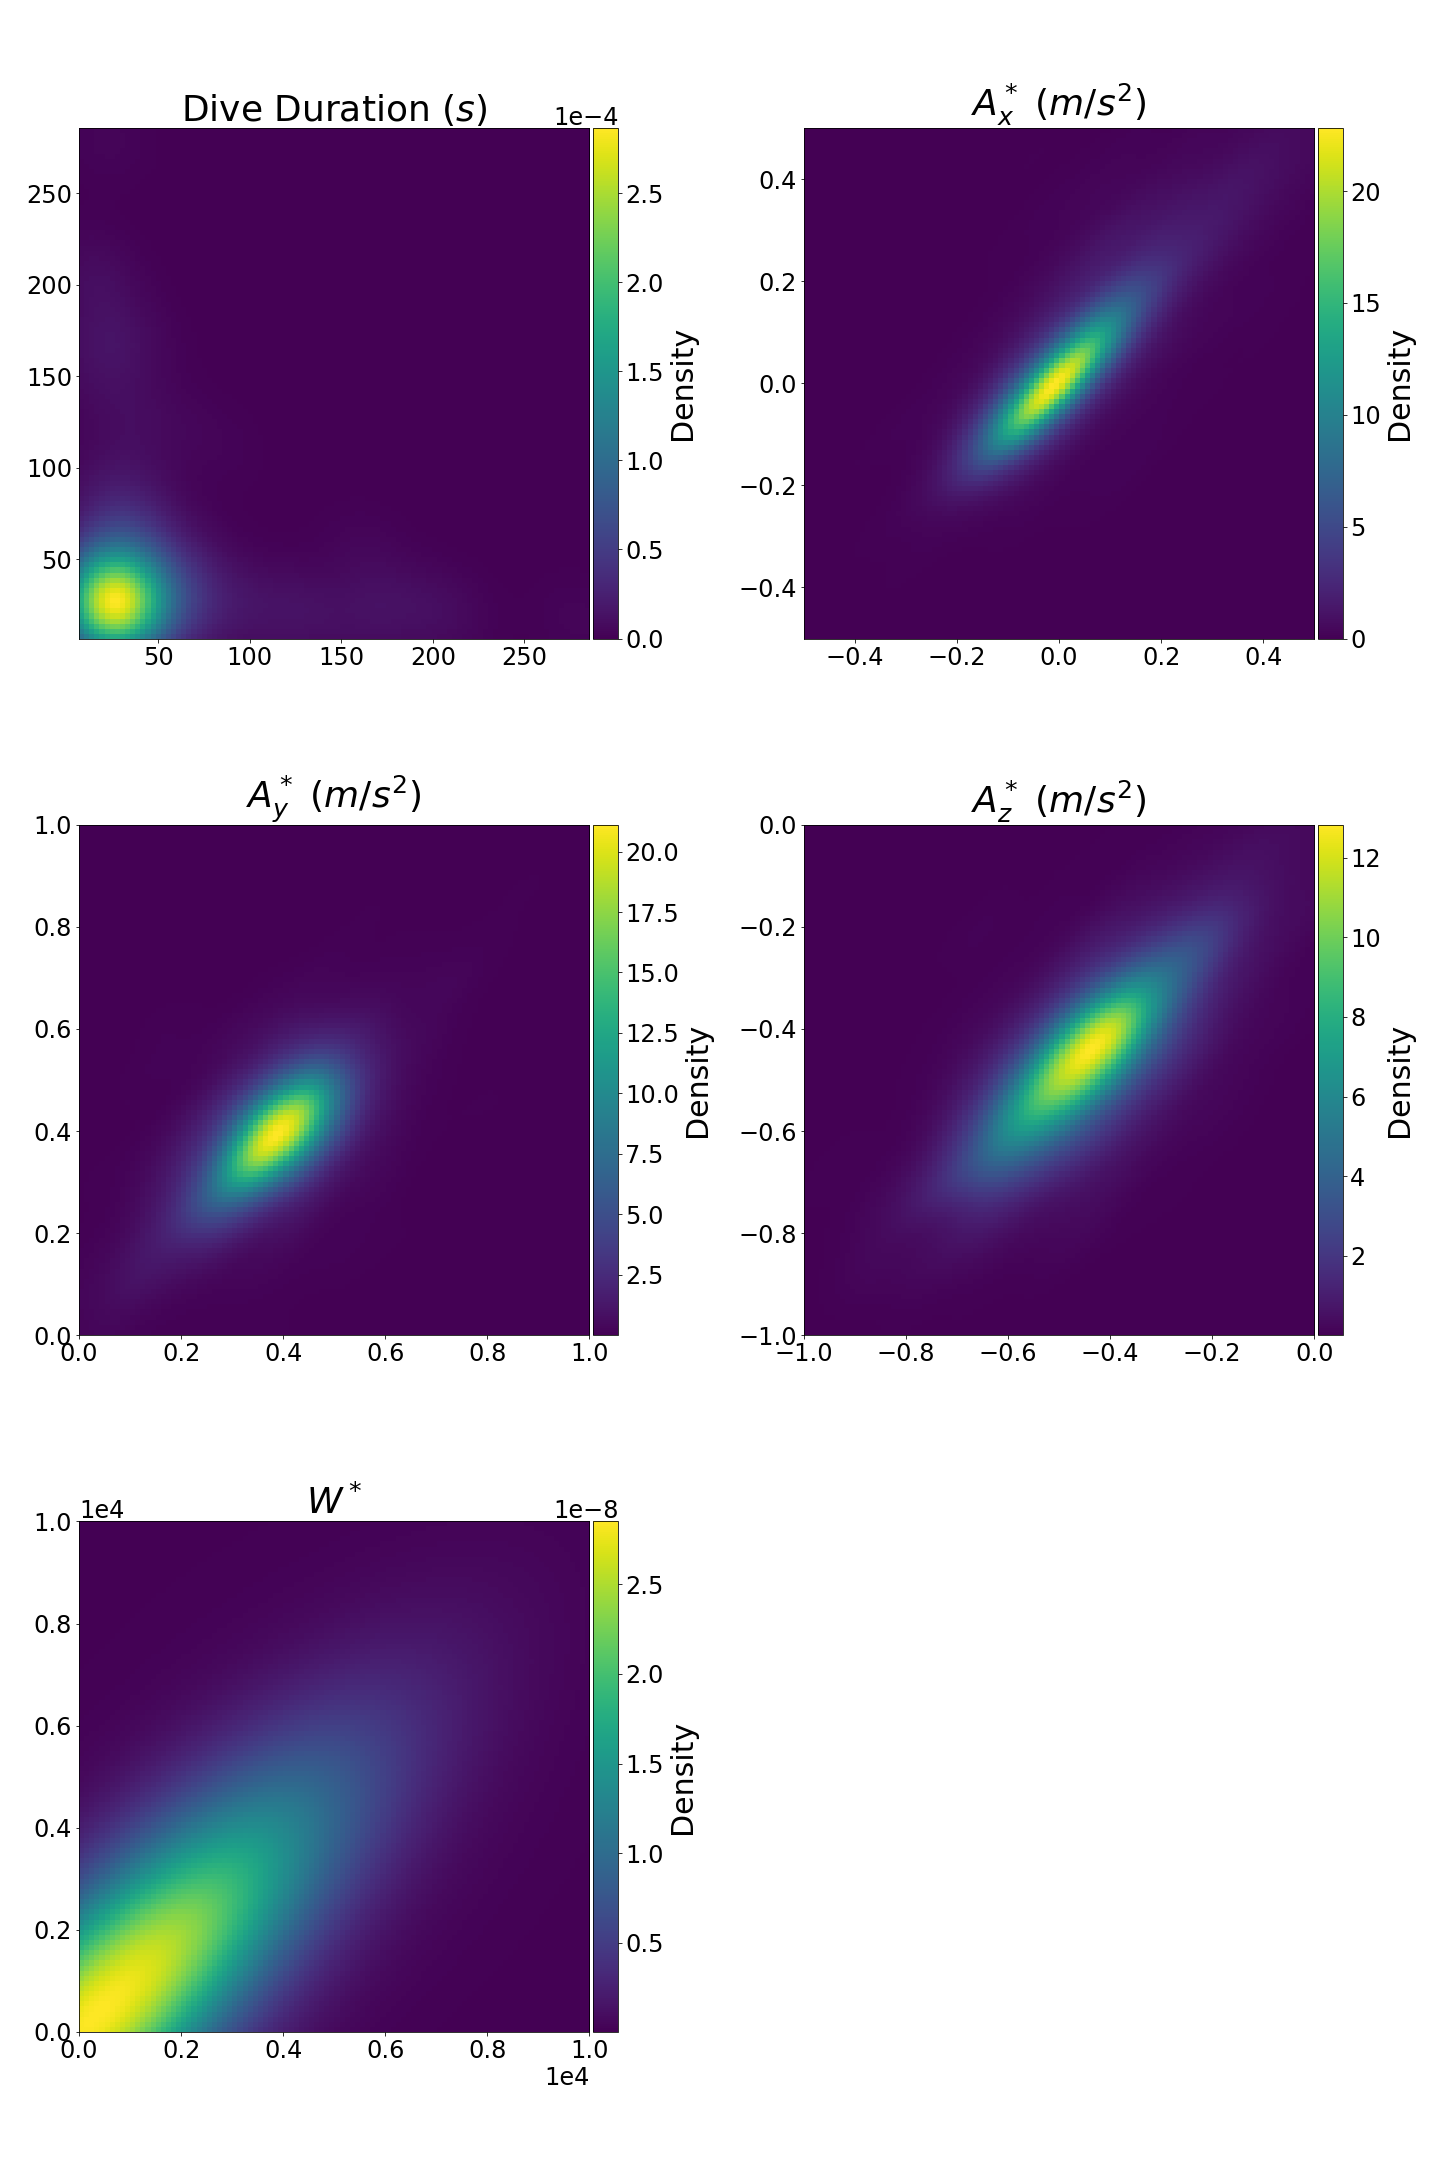
\includegraphics[height=5in]{../Plots/CarHHMM2_lagplot.png}
        \end{center}
        
        \noindent Figure \arabic{fignum}: Collection of 5 lag plots where each one corresponds to a feature in the killer whale dive data. These lag plots are used to decide whether or not to include auto-correlation in the HMMs used to model the killer whale's movement.
        \addtocounter{fignum}{1}
        
        \newpage
    
    \subsection{Parameter Estimates}

        \subsubsection{CarHHMM-DFT}
        
            %\begin{table}[ht]
            %
            %\caption{Estimates and empirical standard errors of emission parameters for dive duration ($Y_t$), acceleration ($\Zone_{t,t^*}$), and willingness ($\Ztwo_{t,t^*}$) of the killer whale case study data under the full CarHHMM-DFT.}
            \begin{center}
            \scalebox{0.75}{
            \bgroup
            \centering
            \def\arraystretch{1.5}
            \begin{tabular}{ccccc}
                \multirow{2}{*}{Feature}                                                       & \multirow{2}{*}{Dive / Subdive Type} & \multicolumn{3}{c}{Parameter Estimate}                     \\
                                                                                               &                                      & $\hat \mu$         & $\hat \sigma$     & $\hat \phi$       \\ \hline
                \multirow{2}{*}{Dive Duration $(s)$ - $Y_t$}                                   & 1                                    & $25.69 \pm 0.60$   & $9.57 \pm 0.51$   & ---               \\
                                                                                               & 2                                    & $104.6 \pm 9.4$    & $64.7 \pm 7.5$    & ---               \\ \hline
                \multirow{3}{*}{X-Acceleration $(m/s^2)$ - $\left(\Zone_{t,t^*}\right)_x$}     & 1                                    & $0.020 \pm 0.042$  & $0.034 \pm 0.001$ & $0.976 \pm 0.007$ \\
                                                                                               & 2                                    & $0.244 \pm 0.013$  & $0.079 \pm 0.001$ & $0.886 \pm 0.005$ \\
                                                                                               & 3                                    & $0.218 \pm 0.028$  & $0.265 \pm 0.007$ & $0.626 \pm 0.029$ \\ \hline
                \multirow{3}{*}{Y-acceleration $(m/s^2)$ - $\left(\Zone_{t,t^*}\right)_y$}     & 1                                    & $0.469 \pm 0.052$  & $0.044 \pm 0.001$ & $0.976 \pm 0.009$ \\
                                                                                               & 2                                    & $0.436 \pm 0.014$  & $0.082 \pm 0.001$ & $0.886 \pm 0.012$ \\
                                                                                               & 3                                    & $0.384 \pm 0.033$  & $0.321 \pm 0.009$ & $0.626 \pm 0.034$ \\ \hline
                \multirow{3}{*}{Z-acceleration $(m/s^2)$ - $\left(\Zone_{t,t^*}\right)_z$}     & 1                                    & $-0.683 \pm 0.061$ & $0.052 \pm 0.001$ & $0.976 \pm 0.005$ \\
                                                                                               & 2                                    & $-0.593 \pm 0.016$ & $0.096 \pm 0.001$ & $0.886 \pm 0.009$ \\
                                                                                               & 3                                    & $-0.366 \pm 0.033$ & $0.317 \pm 0.009$ & $0.626 \pm 0.033$ \\ \hline
                \multirow{3}{*}{Wiggliness - $\Ztwo_{t,t^*}$}                                  & 1                                    & $23.34 \pm 0.28$   & $12.95 \pm 0.27$  & ---               \\
                                                                                               & 2                                    & $301.2 \pm 3.2$    & $330.1 \pm 4.2$   & ---               \\
                                                                                               & 3                                    & $10200 \pm 210$    & $15300 \pm 350$   & ---               \\ \hline
                \end{tabular}
                \egroup
                }
                \end{center}
                
                \noindent Table \arabic{tablenum}: Estimates and empirical standard errors of emission parameters for dive duration ($Y_t$), acceleration ($\Zone_{t,t^*}$), and willingness ($\Ztwo_{t,t^*}$) of the killer whale case study data under the full CarHHMM-DFT. The $\pm$ refers to the standard deviation of the parameter estimates across all 500 data simulations.
                \addtocounter{tablenum}{1}
    
        \subsubsection{HHMM-DFT}
            \begin{center}
            \scalebox{0.75}{
                \bgroup
                \centering
                \def\arraystretch{1.5}
                \begin{tabular}{ccccc}
                \multirow{2}{*}{Feature}                                                       & \multirow{2}{*}{Dive / Subdive Type} & \multicolumn{3}{c}{Parameter Estimate}                   \\
                                                                                               &                                      & $\hat \mu$         & $\hat \sigma$     & $\hat \phi$     \\ \hline
                \multirow{2}{*}{Dive Duration $(s)$ - $Y_t$}                                   & 1                                    & $25.34 \pm 0.60$   & $8.82 \pm 0.51$   & ---             \\
                                                                                               & 2                                    & $92.7 \pm 7.7$     & $63.7 \pm 6.5$    & ---             \\ \hline
                \multirow{3}{*}{X-Acceleration $(m/s^2)$ - $\left(\Zone_{t,t^*}\right)_x$}     & 1                                    & $-0.023 \pm 0.002$ & $0.053 \pm 0.001$ & ---             \\
                                                                                               & 2                                    & $0.074 \pm 0.003$  & $0.149 \pm 0.002$ & ---             \\
                                                                                               & 3                                    & $0.214 \pm 0.014$  & $0.422 \pm 0.010$ & ---             \\ \hline
                \multirow{3}{*}{Y-Acceleration $(m/s^2)$ - $\left(\Zone_{t,t^*}\right)_y$}     & 1                                    & $0.342 \pm 0.002$  & $0.064 \pm 0.002$ & ---             \\
                                                                                               & 2                                    & $0.408 \pm 0.002$  & $0.091 \pm 0.001$ & ---             \\
                                                                                               & 3                                    & $0.320 \pm 0.011$  & $0.341 \pm 0.008$ & ---             \\ \hline
                \multirow{3}{*}{Z-Acceleration $(m/s^2)$ - $\left(\Zone_{t,t^*}\right)_z$}     & 1                                    & $-0.418 \pm 0.003$ & $0.104 \pm 0.002$ & ---             \\
                                                                                               & 2                                    & $-0.478 \pm 0.003$ & $0.136 \pm 0.002$ & ---             \\
                                                                                               & 3                                    & $-0.346 \pm 0.012$ & $0.359 \pm 0.008$ & ---             \\ \hline
                \multirow{3}{*}{Wiggliness - $\Ztwo_{t,t^*}$}                                  & 1                                    & $25.32 \pm 0.38$   & $15.94 \pm 0.38$  & ---             \\
                                                                                               & 2                                    & $252.4 \pm 2.8$    & $296.9 \pm 3.9$   & ---             \\
                                                                                               & 3                                    & $8800 \pm 150$     & $15580 \pm 290$   & ---             \\ \hline
                \end{tabular}
                \egroup
            }
            \end{center}
            
            \noindent Table \arabic{tablenum}: Estimates and empirical standard errors of emission parameters for dive duration ($Y_t$), acceleration ($\Zone_{t,t^*}$), and willingness ($\Ztwo_{t,t^*}$) of the killer whale case study data under the HHMM-DFT. The $\pm$ refers to the standard deviation of the parameter estimates across all 500 data simulations.
            \addtocounter{tablenum}{1}
            
        \subsubsection{CarHHMM}
            
            \begin{center}
            \scalebox{0.75}{
                \bgroup
                \centering
                \def\arraystretch{1.5}
                \begin{tabular}{ccccc}
                \multirow{2}{*}{Feature}                                                       & \multirow{2}{*}{Dive / Subdive Type} & \multicolumn{3}{c}{Parameter Estimate}                     \\
                                                                                               &                                      & $\hat \mu$         & $\hat \sigma$     & $\hat \phi$       \\ \hline
                \multirow{2}{*}{Dive Duration $(s)$ - $Y_t$}                                   & 1                                    & $27.21 \pm 0.67$   & $11.64 \pm 0.70$  & ---               \\
                                                                                               & 2                                    & $136 \pm 11$       & $63.8 \pm 9.4$    & ---               \\ \hline
                \multirow{3}{*}{X-Acceleration $(m/s^2)$ - $\left(\Zone_{t,t^*}\right)_x$}     & 1                                    & $-0.061 \pm 0.088$ & $0.392 \pm 0.019$ & $0.725 \pm 0.045$ \\
                                                                                               & 2                                    & $0.228 \pm 0.017$  & $0.043 \pm 0.001$ & $0.945 \pm 0.004$ \\
                                                                                               & 3                                    & $0.172 \pm 0.012$  & $0.129 \pm 0.003$ & $0.721 \pm 0.017$ \\ \hline
                \multirow{3}{*}{Y-Acceleration $(m/s^2)$ - $\left(\Zone_{t,t^*}\right)_y$}     & 1                                    & $0.38 \pm 0.12$    & $0.552 \pm 0.033$ & $0.725 \pm 0.064$ \\
                                                                                               & 2                                    & $0.387 \pm 0.020$  & $0.052 \pm 0.001$ & $0.945 \pm 0.011$ \\
                                                                                               & 3                                    & $0.441 \pm 0.011$  & $0.118 \pm 0.002$ & $0.721 \pm 0.023$ \\ \hline
                \multirow{3}{*}{Z-Acceleration $(m/s^2)$ - $\left(\Zone_{t,t^*}\right)_z$}     & 1                                    & $-0.44 \pm 0.11$   & $0.506 \pm 0.028$ & $0.725 \pm 0.055$ \\
                                                                                               & 2                                    & $-0.537 \pm 0.023$ & $0.059 \pm 0.001$ & $0.945 \pm 0.008$ \\
                                                                                               & 3                                    & $-0.561 \pm 0.012$ & $0.135 \pm 0.003$ & $0.721 \pm 0.018$ \\ \hline
                \end{tabular}
                \egroup
            }
            \end{center}
            
                \noindent Table \arabic{tablenum}: Estimates and empirical standard errors of emission parameters for dive duration ($Y_t$) and acceleration ($\Zone_{t,t^*}$) of the killer whale case study data under the CarHHMM. The $\pm$ refers to the standard deviation of the parameter estimates across all 500 data simulations.
                \addtocounter{tablenum}{1}
            
        \subsubsection{CarHMM-DFT}
            
            \begin{center}
            \scalebox{0.75}{
                \bgroup
                \centering
                \def\arraystretch{1.5}
                \begin{tabular}{ccccc}
                \multirow{2}{*}{Feature}                                                       & \multirow{2}{*}{Dive / Subdive Type} & \multicolumn{3}{c}{Parameter Estimate}                     \\
                                                                                               &                                      & $\hat \mu$         & $\hat \sigma$     & $\hat \phi$       \\ \hline
                \multirow{1}{*}{Dive Duration $(s)$ - $Y_t$}                                   & 1                                    & $42.9 \pm 1.3$     & $31.4 \pm 1.3$    & ---               \\ \hline
                \multirow{3}{*}{X-Acceleration $(m/s^2)$ - $\left(\Zone_{t,t^*}\right)_x$}     & 1                                    & Undefined          & $0.035 \pm 0.001$ & $1.000 \pm 0.000$ \\
                                                                                               & 2                                    & $0.241 \pm 0.012$  & $0.084 \pm 0.001$ & $0.861 \pm 0.006$ \\
                                                                                               & 3                                    & $0.208 \pm 0.028$  & $0.266 \pm 0.008$ & $0.619 \pm 0.031$ \\ \hline
                \multirow{3}{*}{Y-Acceleration $(m/s^2)$ - $\left(\Zone_{t,t^*}\right)_y$}     & 1                                    & Undefined          & $0.046 \pm 0.001$ & $1.000 \pm 0.000$ \\
                                                                                               & 2                                    & $0.440 \pm 0.012$  & $0.086 \pm 0.001$ & $0.861 \pm 0.014$ \\
                                                                                               & 3                                    & $0.383 \pm 0.033$  & $0.322 \pm 0.009$ & $0.619 \pm 0.034$ \\ \hline
                \multirow{3}{*}{Z-Acceleration $(m/s^2)$ - $\left(\Zone_{t,t^*}\right)_z$}     & 1                                    & Undefined          & $0.053 \pm 0.001$ & $1.000 \pm 0.000$ \\
                                                                                               & 2                                    & $-0.593 \pm 0.015$ & $0.101 \pm 0.002$ & $0.861 \pm 0.010$ \\
                                                                                               & 3                                    & $-0.355 \pm 0.033$ & $0.318 \pm 0.009$ & $0.619 \pm 0.033$ \\ \hline
                \multirow{3}{*}{Wiggliness  - $\Ztwo_{t,t^*}$}                                 & 1                                    & $24.07 \pm 0.29$   & $13.61 \pm 0.28$  & ---               \\
                                                                                               & 2                                    & $291.6 \pm 3.2$    & $308.2 \pm 4.1$   & ---               \\
                                                                                               & 3                                    & $10210 \pm 200$    & $15010 \pm 340$   & ---               \\ \hline
                \end{tabular}
                \egroup
            }
            \end{center}
            
                \noindent Table \arabic{tablenum}: Estimates and empirical standard errors of emission parameters for dive duration ($Y_t$), acceleration ($\Zone_{t,t^*}$), and willingness ($\Ztwo_{t,t^*}$) of the killer whale case study data under the CarHMM-DFT. The $\pm$ refers to the standard deviation of the parameter estimates across all 500 data simulations. Note that $\hat \mu_A^{*(\cdot,1)}$ is undefined because $\hat \phi_A^{*(\cdot,1)} = 1$, indicating that the mean of $\Zone_{t,t^*}$ is equal to $\Zone_{t,t^*-1}$ when in subdive state 1.
                \addtocounter{tablenum}{1}
    
    \newpage
    \subsection{Decoded dive states}
    
        \subsubsection{CarHHMM-DFT}
        
        \begin{center}
        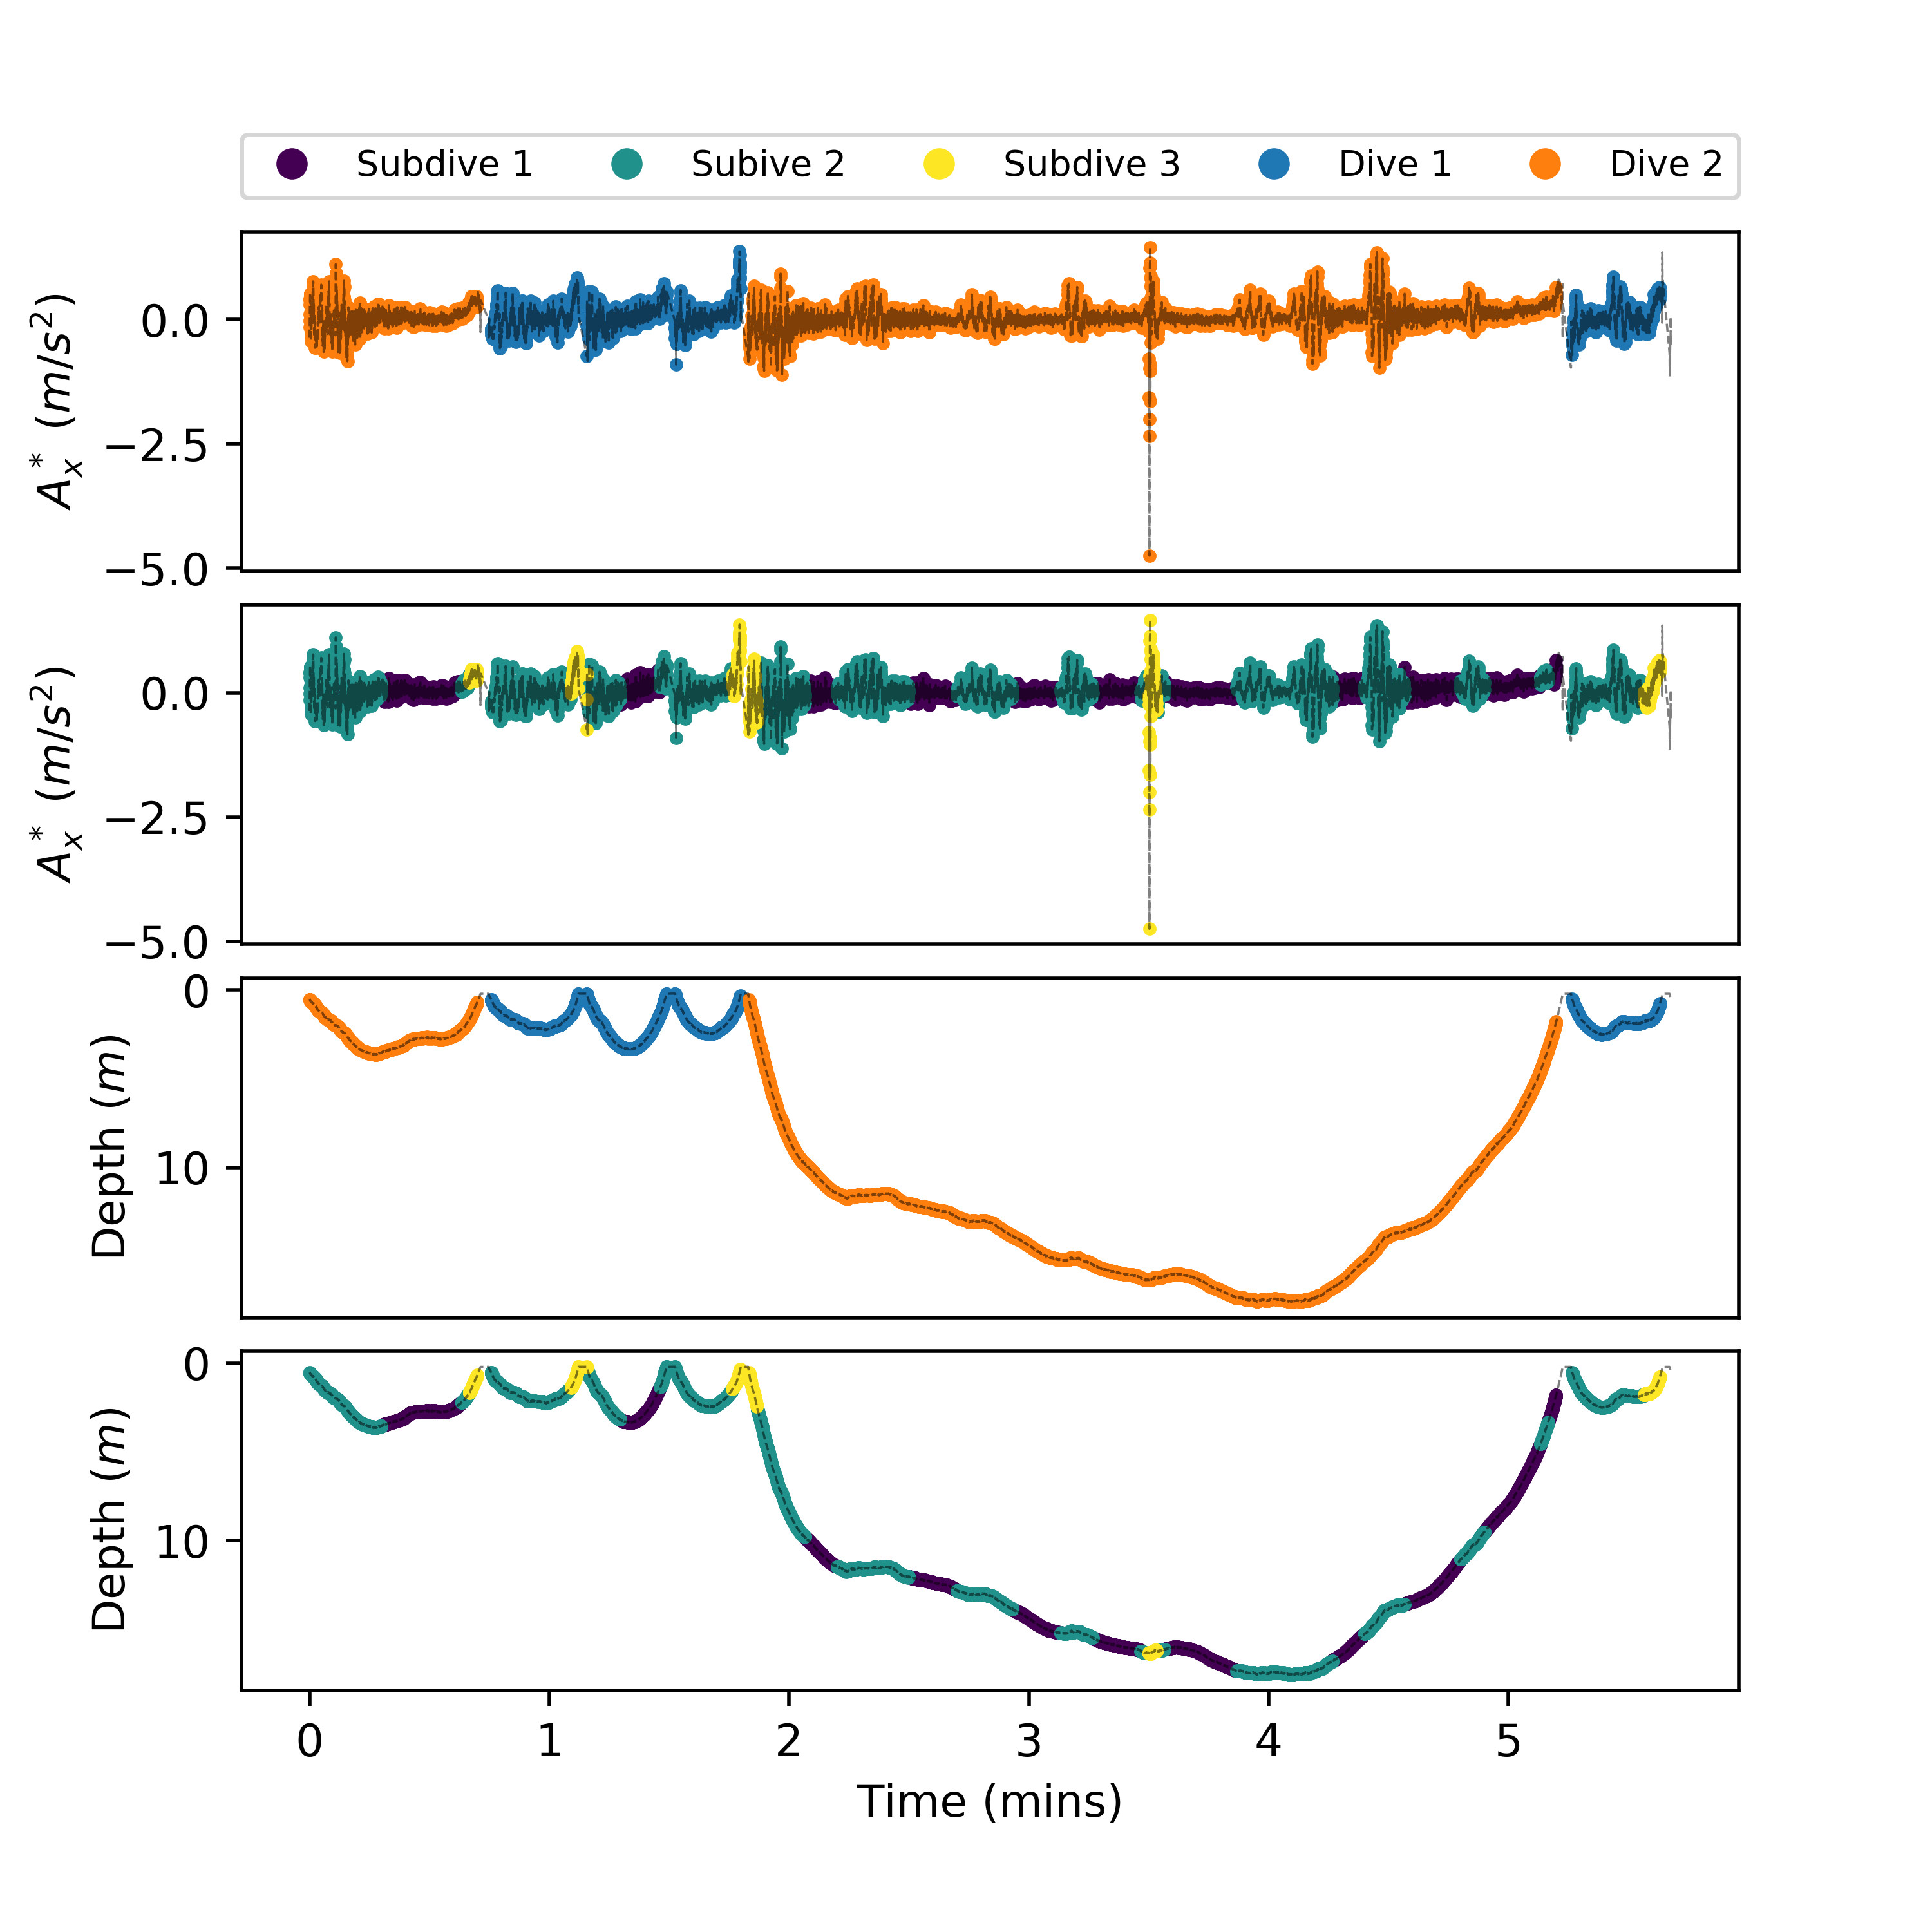
\includegraphics[width=6in]{../Plots/CarHHMM2_decoded_dives.png}
        \end{center}
        
        \noindent Figure \arabic{fignum}: The $x$-component of acceleration $\left(y^*_{t,t^*}\right)_x$ and dive profile of a northern resident killer whale for dives $t = 160,161,162,163,164,$ and $165$. The line colour of the first and third panels corresponds to the estimated dive type while the line colour of the second and fourth panels corresponds to the estimated subdive state. Both the dive types and subdive states are estimated by fitting the CarHHMM-DFT to the data.
        \addtocounter{fignum}{1}
        
        \begin{center}
        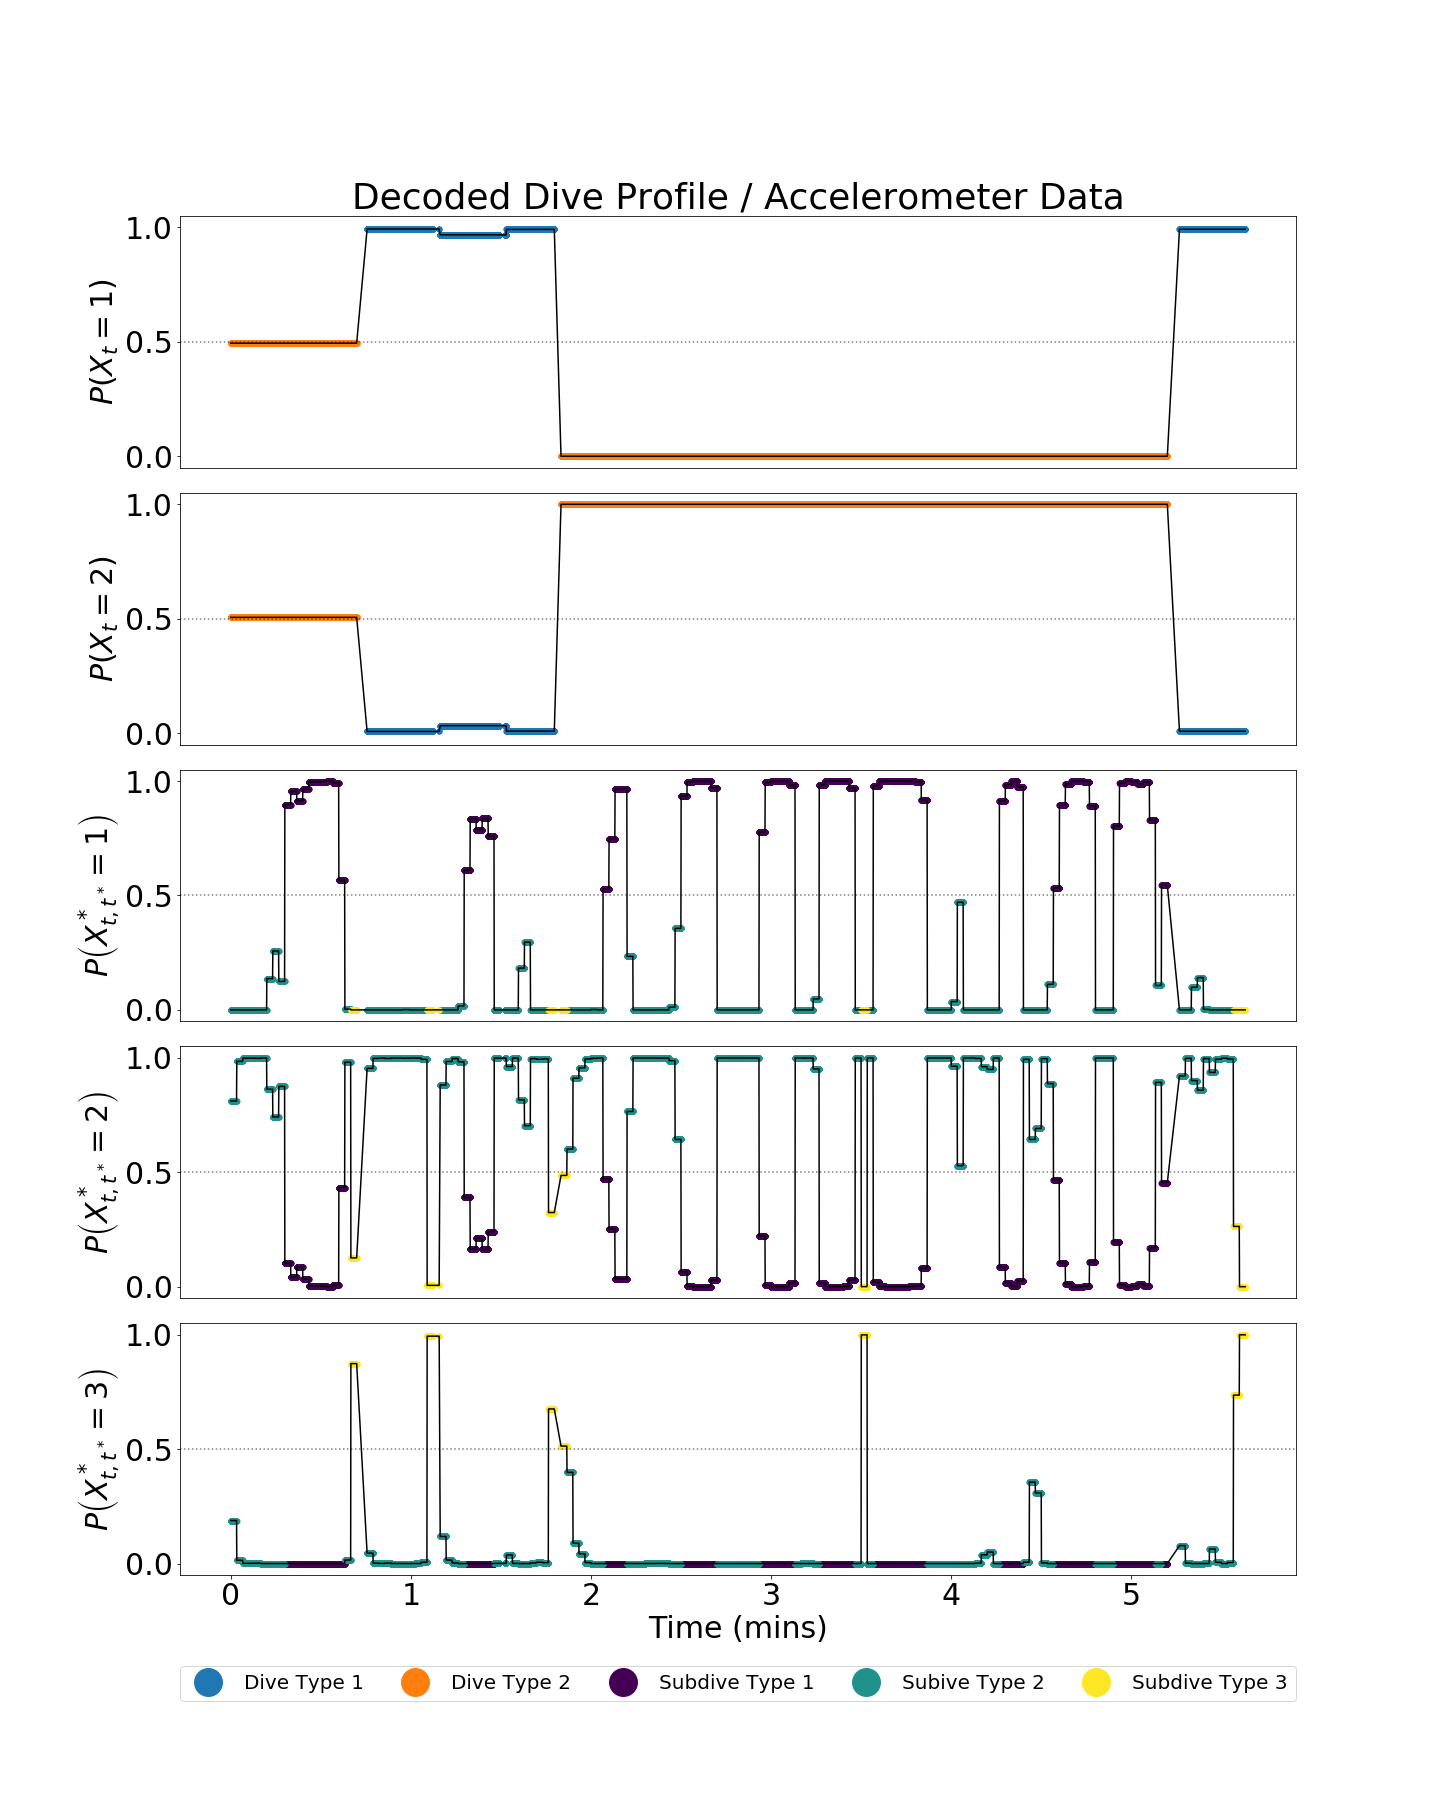
\includegraphics[width=6in]{../Plots/CarHHMM2_decoded_states.png}
        \end{center}
        
        \noindent Figure \arabic{fignum}: The probability that each dive is a particular type or that the whale is in a particular subdive state, given the fitted model. This is shown for dives $t = 160,161,162,163,164,$ and $165$. The line colour of the first two panels corresponds to the estimated dive type while the line colour of the last three panels corresponds to the estimated subdive state. Both the dive types and subdive states are estimated by fitting the CarHHMM-DFT to the data.
        \addtocounter{fignum}{1}
        
        \subsubsection{HHMM-DFT}
        
        \begin{center}
        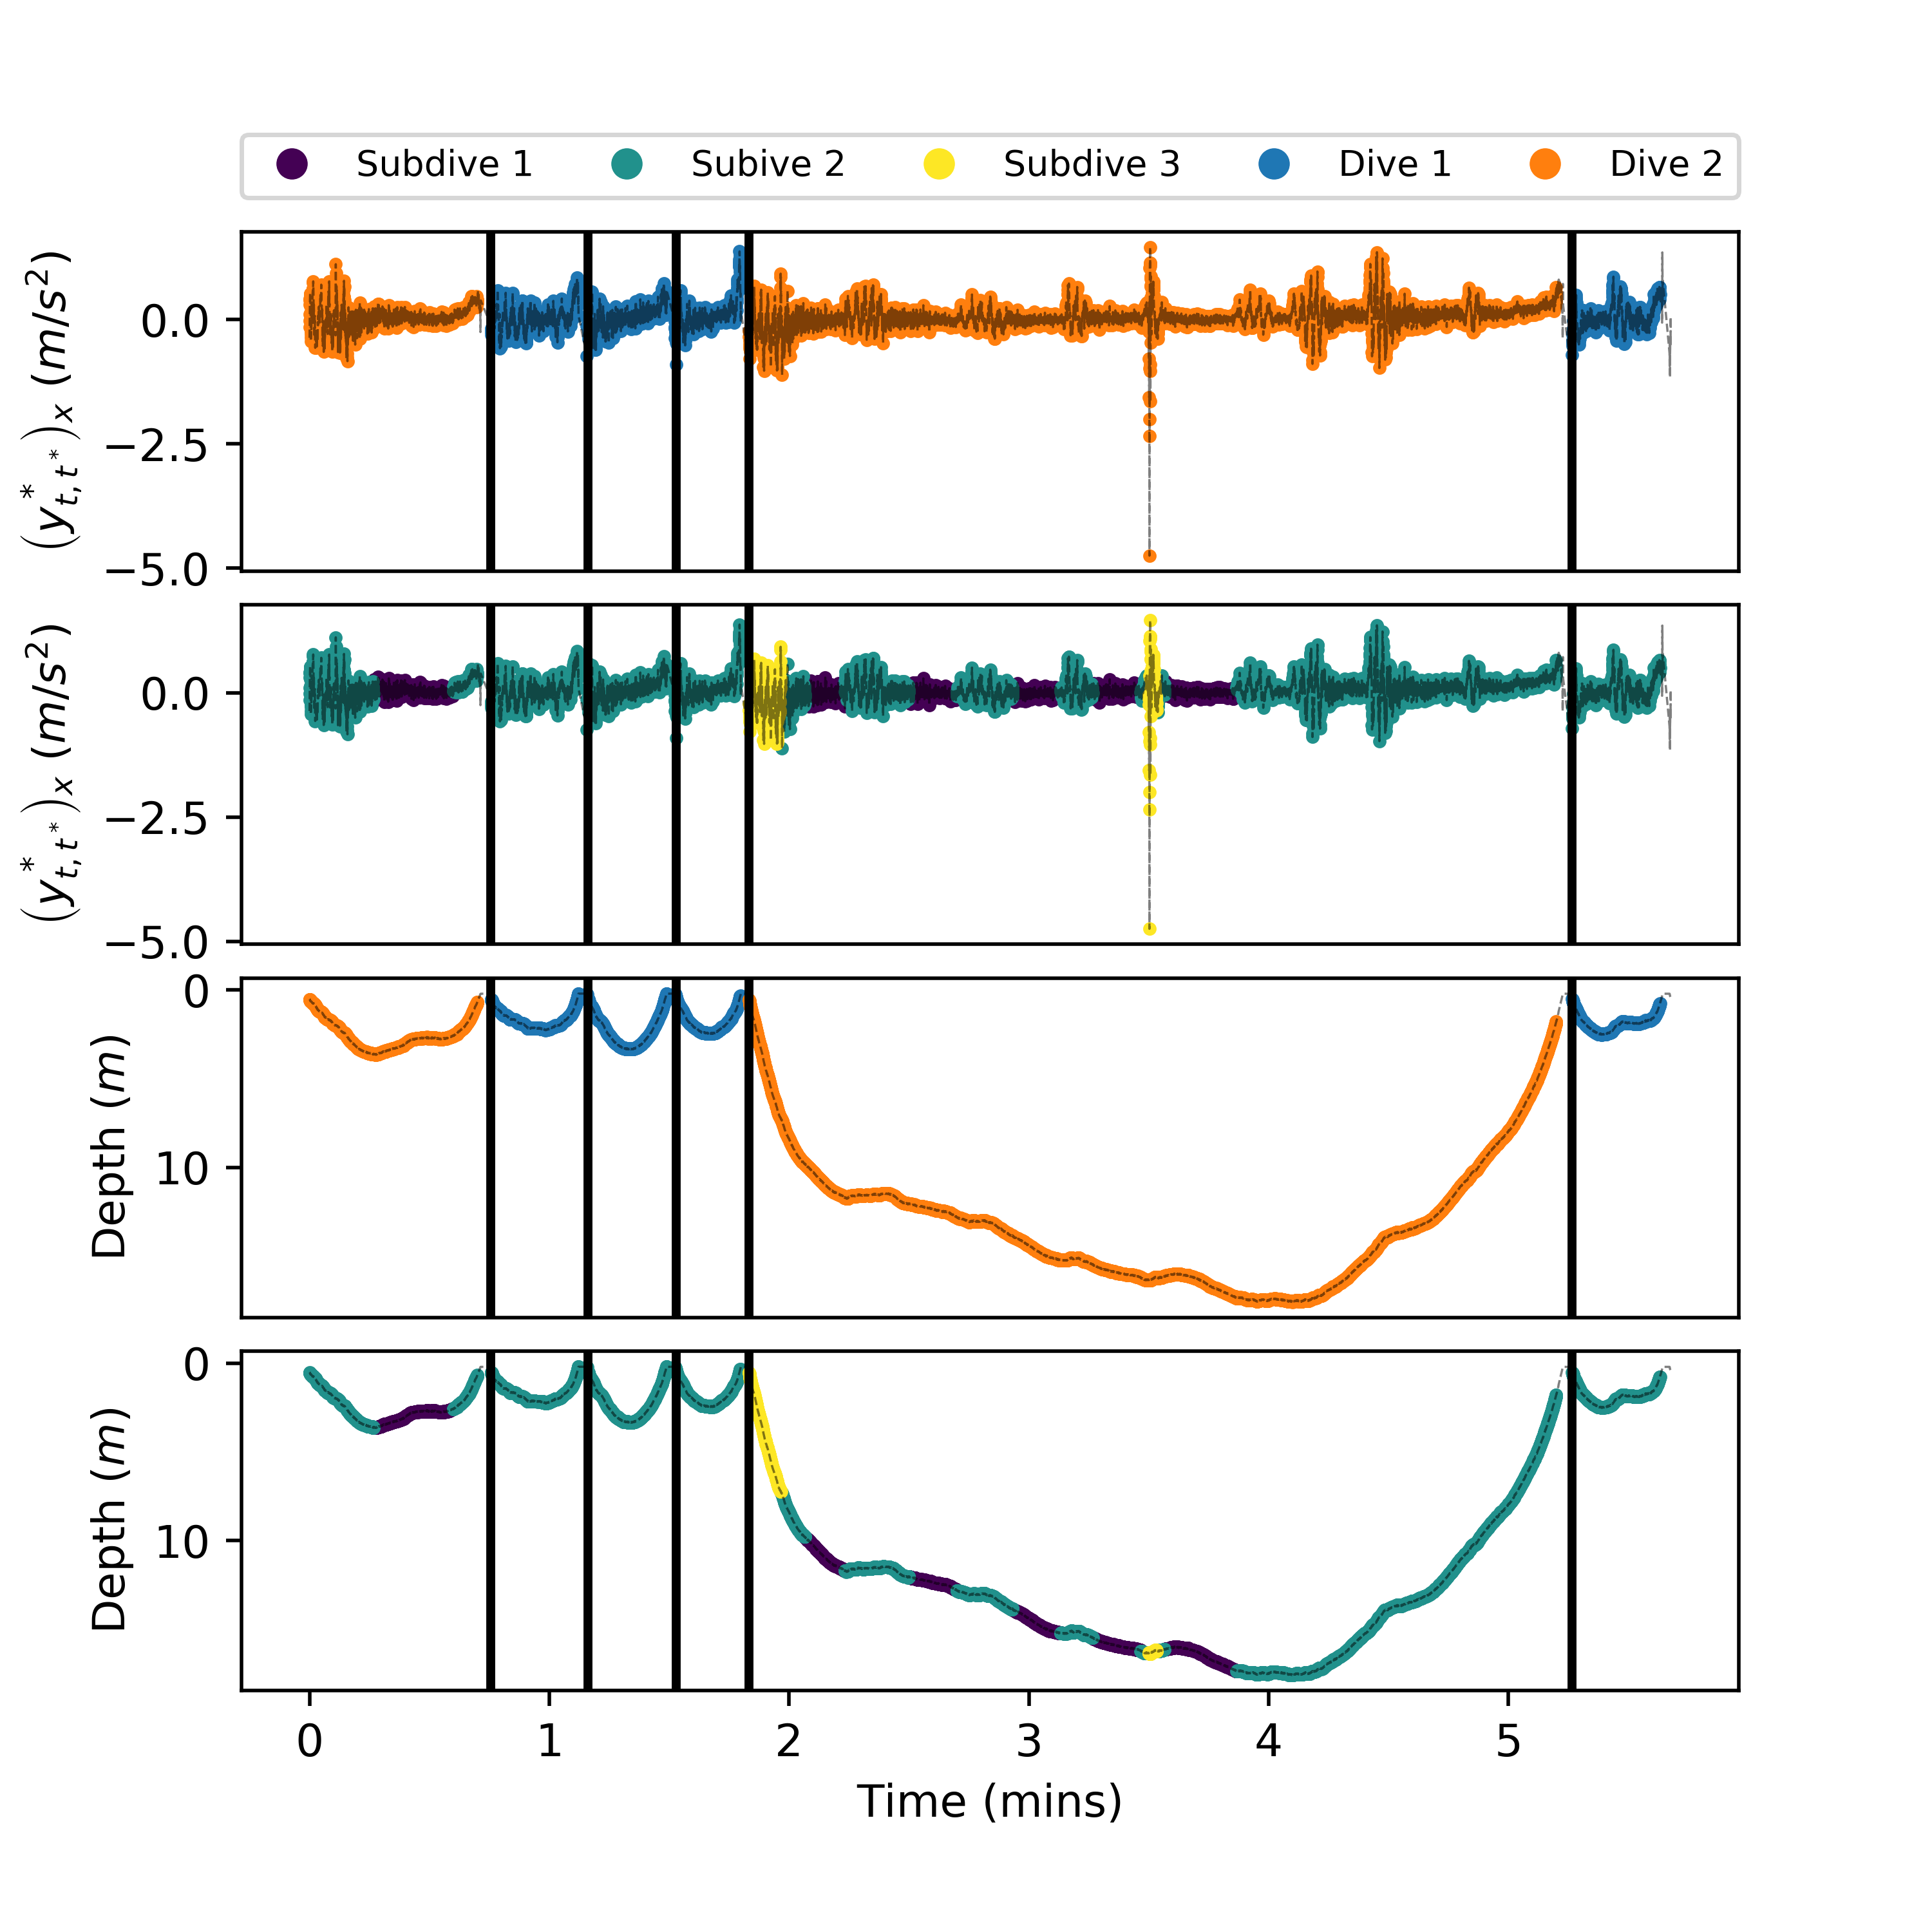
\includegraphics[width=6in]{../Plots/HHMM_decoded_dives.png}
        \end{center}
        
        \noindent Figure \arabic{fignum}: The $x$-component of acceleration $\left(y^*_{t,t^*}\right)_x$ and dive profile of a northern resident killer whale for dives $t = 160,161,162,163,164,$ and $165$. The line colour of the first and third panels corresponds to the estimated dive type while the line colour of the second and fourth panels corresponds to the estimated subdive state. Both the dive types and subdive states are estimated by fitting the HHMM-DFT to the data.
        \addtocounter{fignum}{1}
        
        \begin{center}
        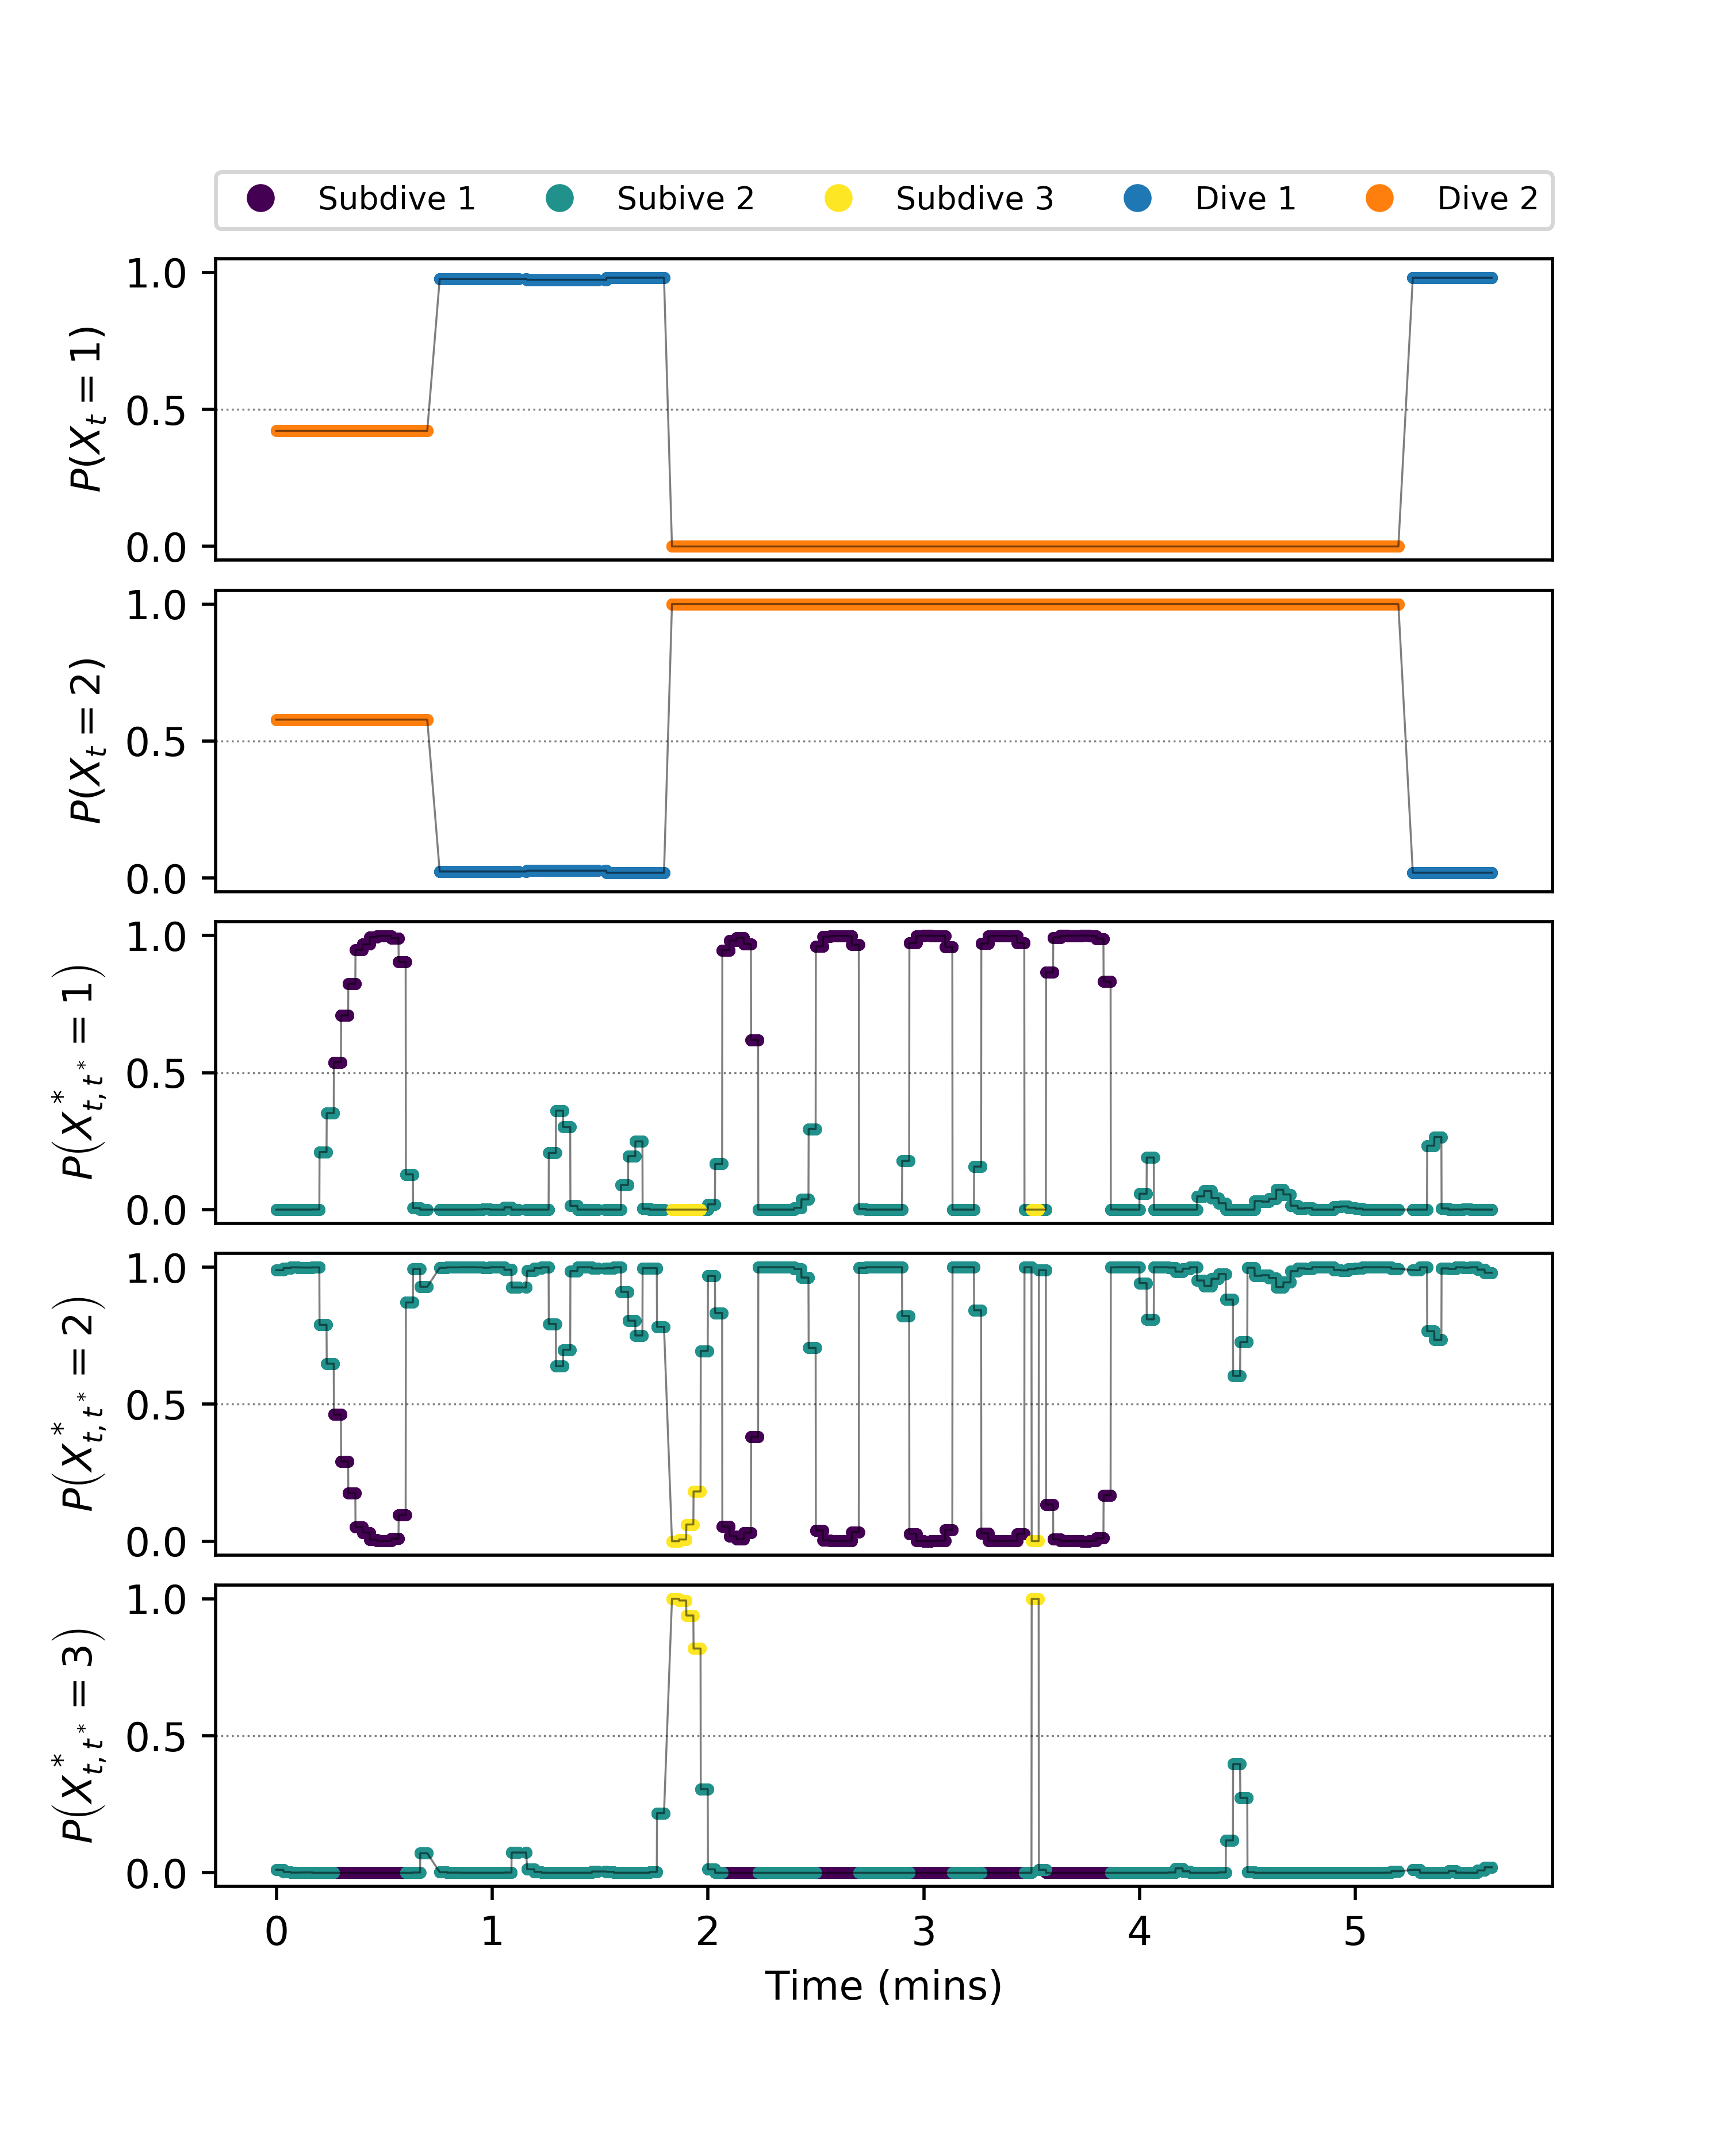
\includegraphics[width=6in]{../Plots/HHMM_decoded_states.png}
        \end{center}
        
        \noindent Figure \arabic{fignum}: The probability that each dive is a particular type or that the whale is in a particular subdive state, given the fitted model. This is shown for dives $t = 160,161,162,163,164,$ and $165$. The line colour of the first two panels corresponds to the estimated dive type while the line colour of the last three panels corresponds to the estimated subdive state. Both the dive types and subdive states are estimated by fitting the CarHHMM-DFT to the data.
        \addtocounter{fignum}{1}
        
        \subsubsection{CarHHMM}
        
        \begin{center}
        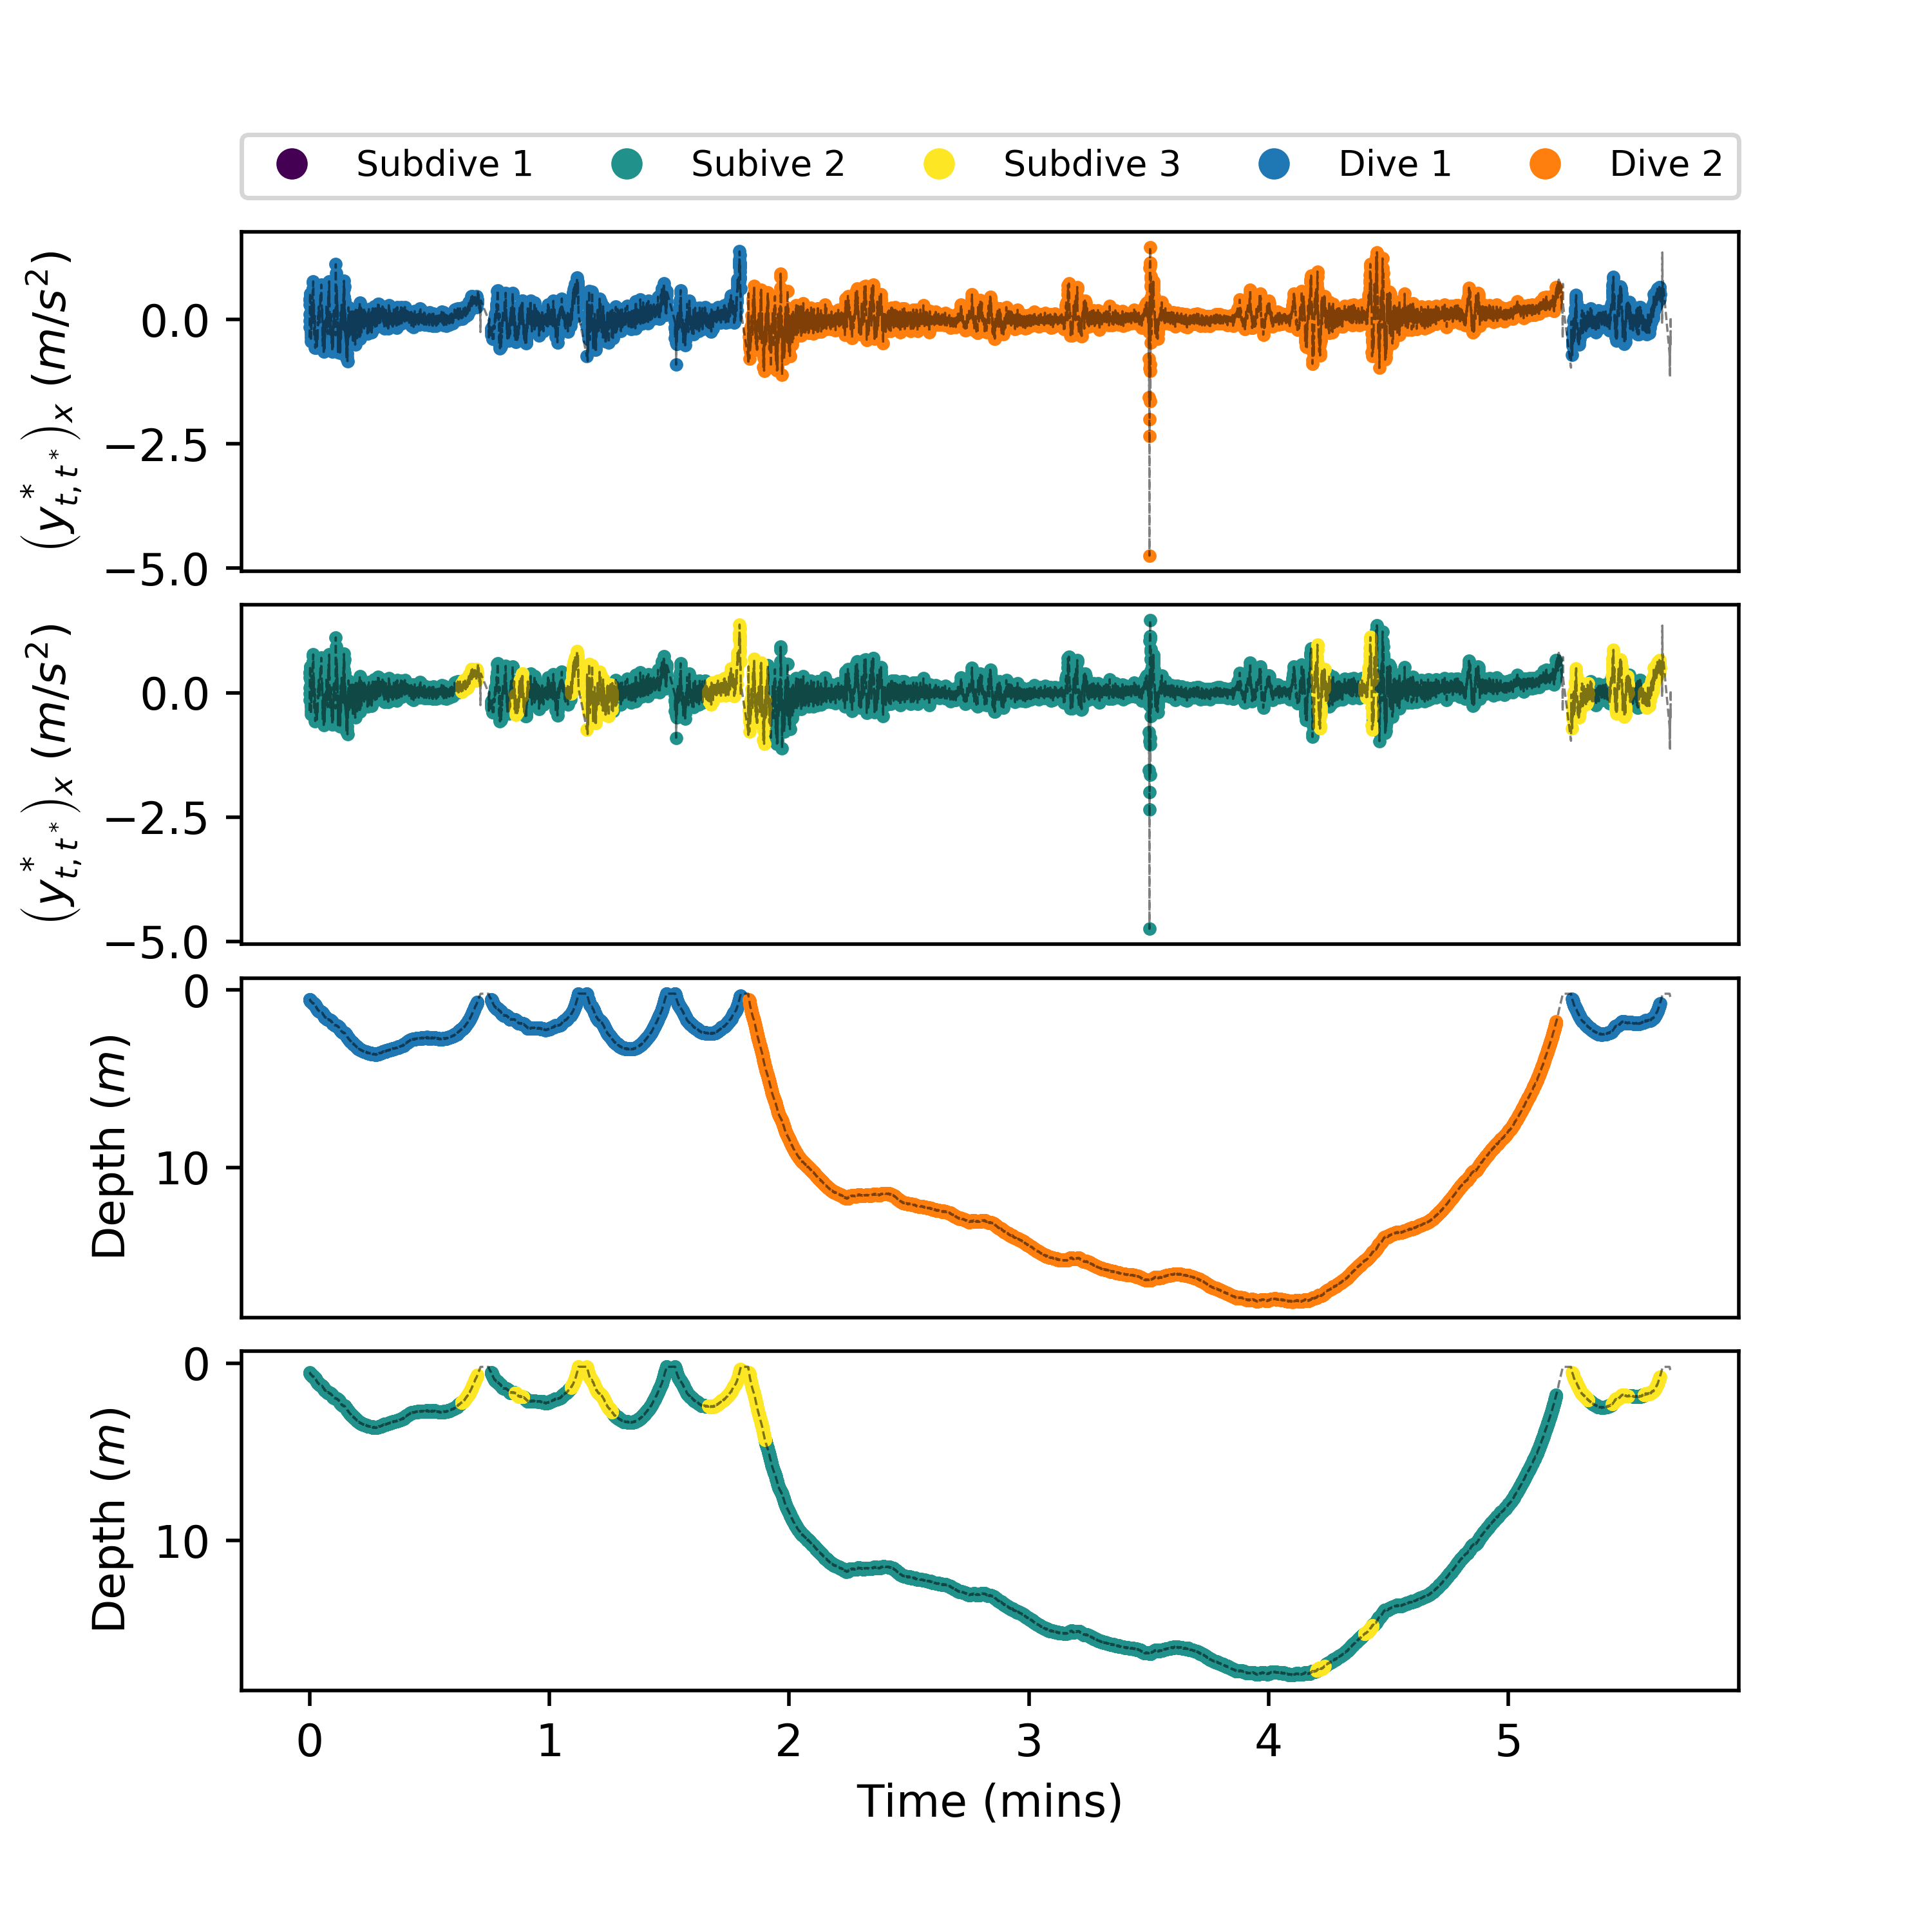
\includegraphics[width=6in]{../Plots/CarHHMM1_decoded_dives.png}
        \end{center}
        
        \noindent Figure \arabic{fignum}: The $x$-component of acceleration $\left(y^*_{t,t^*}\right)_x$ and dive profile of a northern resident killer whale for dives $t = 160,161,162,163,164,$ and $165$. The line colour of the first and third panels corresponds to the estimated dive type while the line colour of the second and fourth panels corresponds to the estimated subdive state. Both the dive types and subdive states are estimated by fitting the CarHHMM to the data.
        \addtocounter{fignum}{1}
        
        \begin{center}
        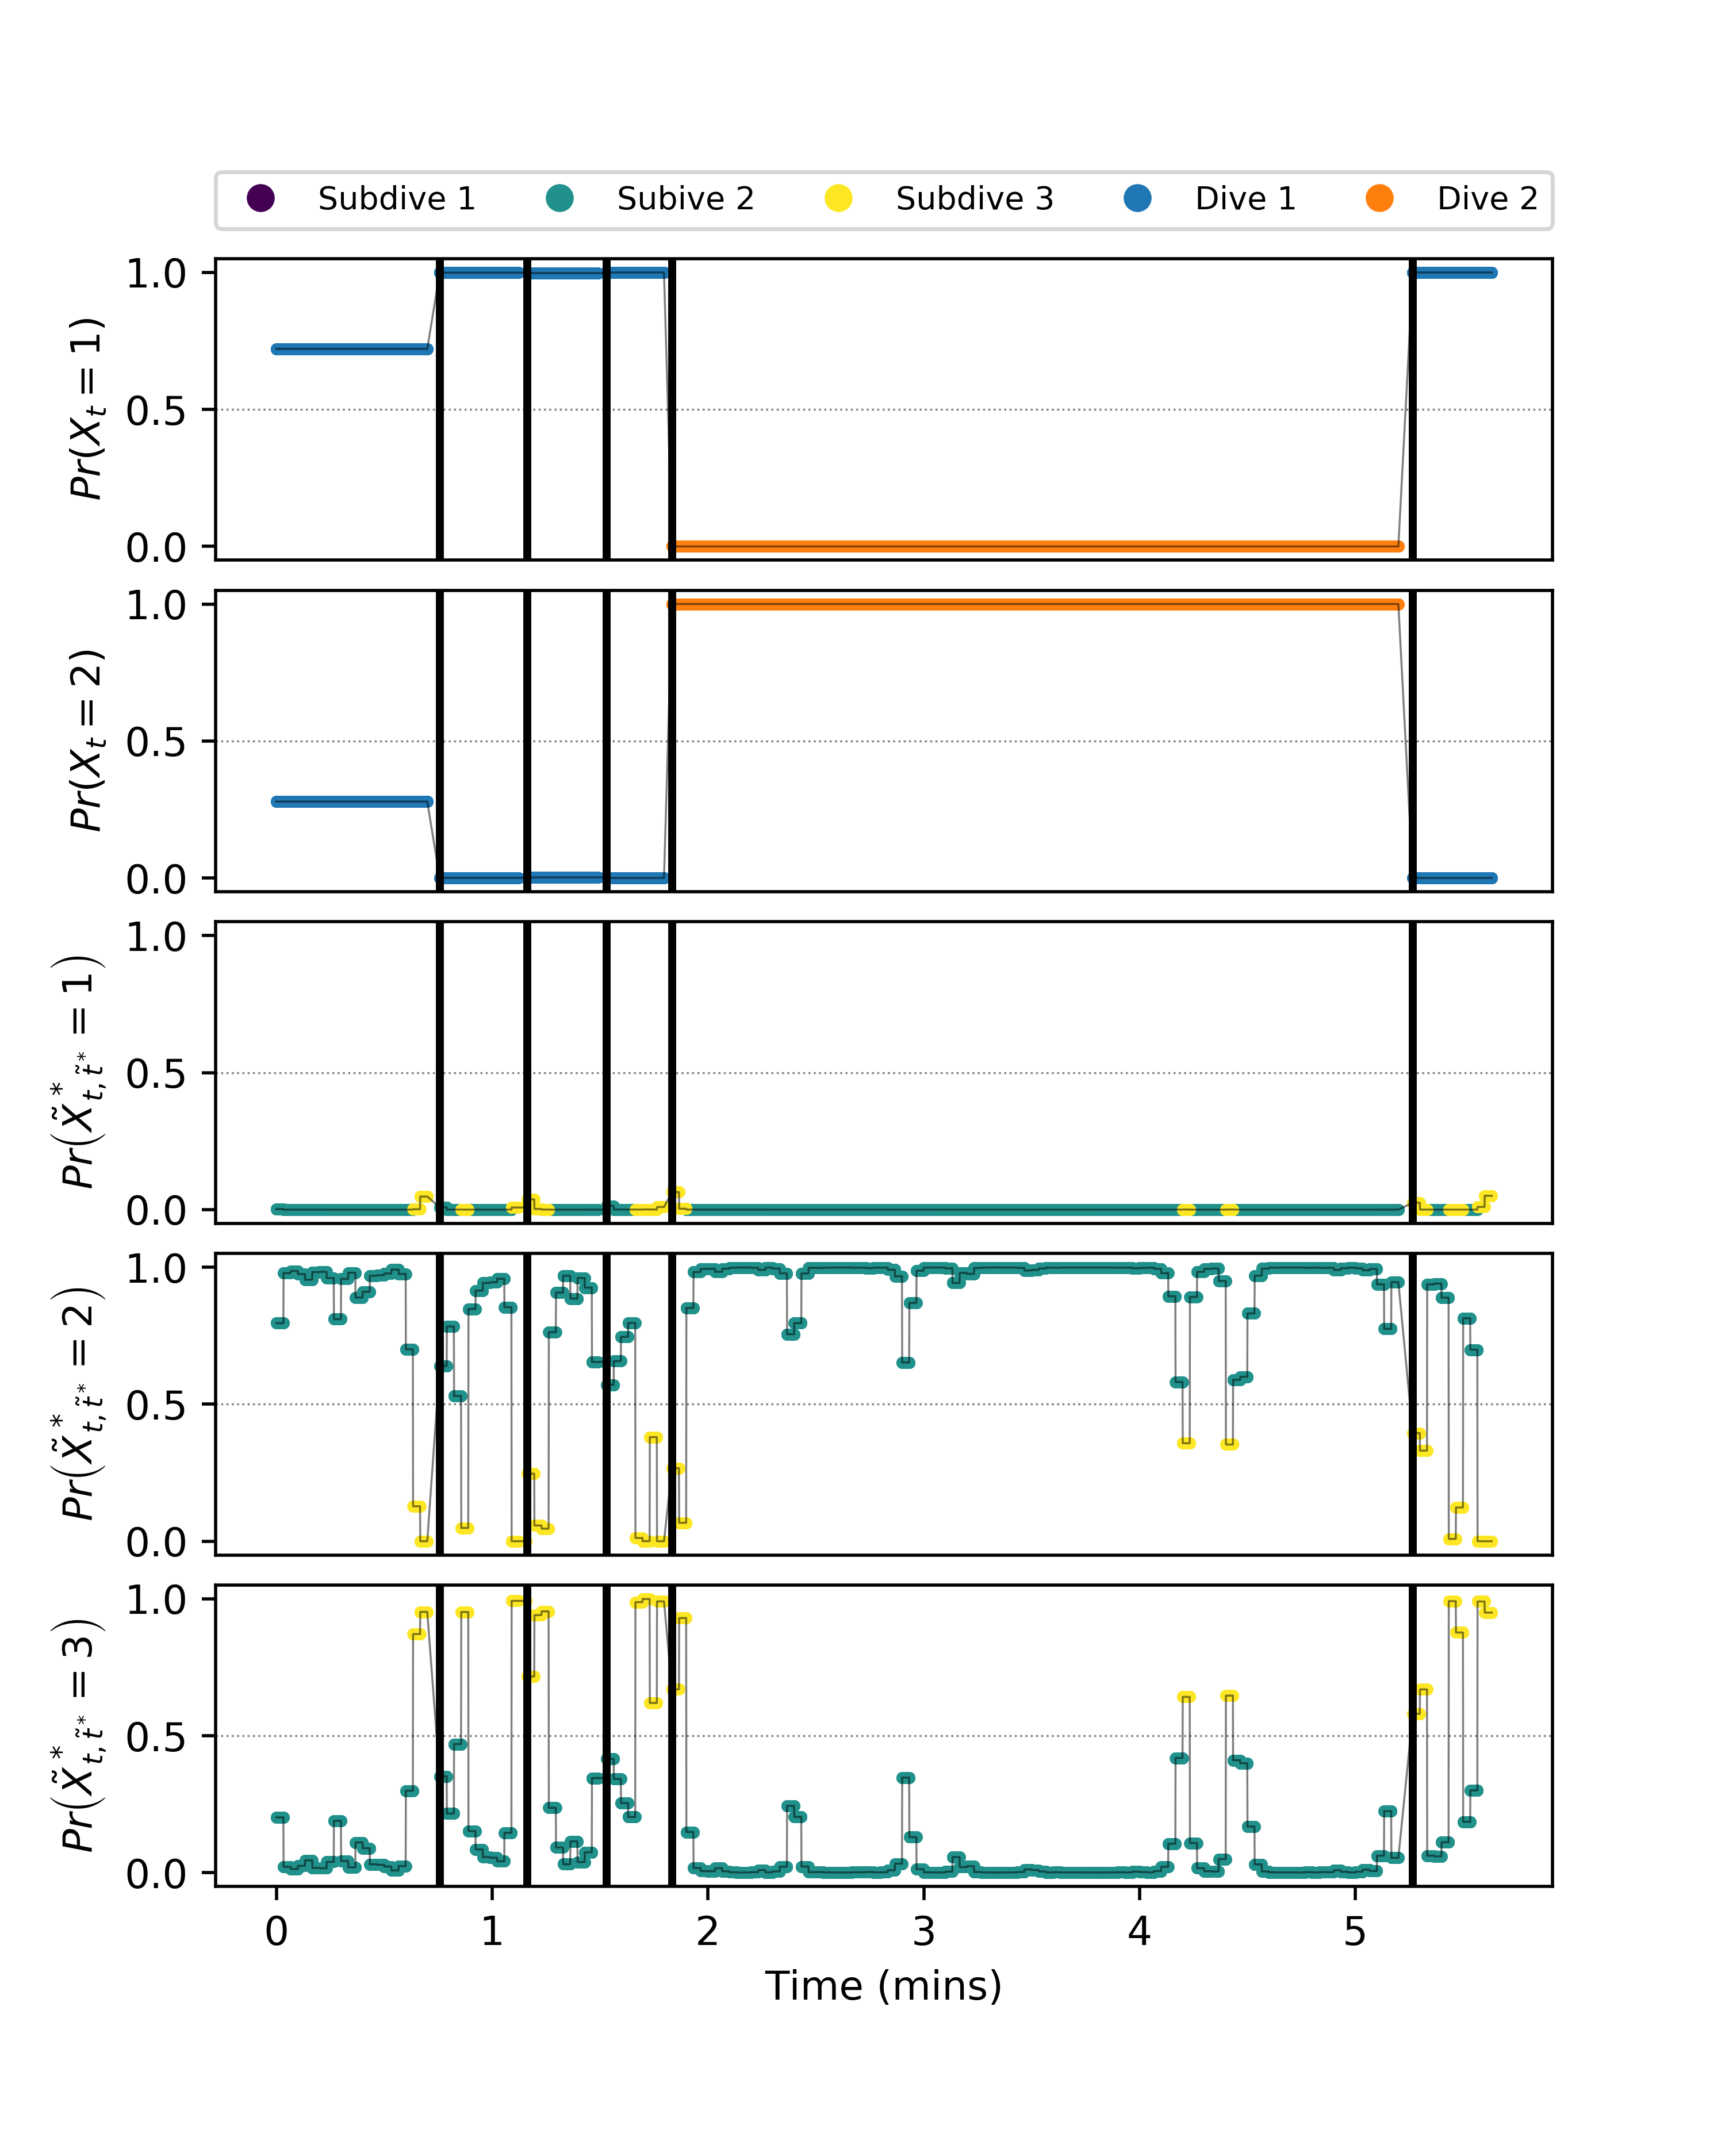
\includegraphics[width=6in]{../Plots/CarHHMM1_decoded_states.png}
        \end{center}
        
        \noindent Figure \arabic{fignum}: The probability that each dive is a particular type or that the whale is in a particular subdive state, given the fitted model. This is shown for dives $t = 160,161,162,163,164,$ and $165$. The line colour of the first two panels corresponds to the estimated dive type while the line colour of the last three panels corresponds to the estimated subdive state. Both the dive types and subdive states are estimated by fitting the CarHHMM-DFT to the data.
        \addtocounter{fignum}{1}
        
        \subsubsection{CarHMM-DFT}
        
        \begin{center}
        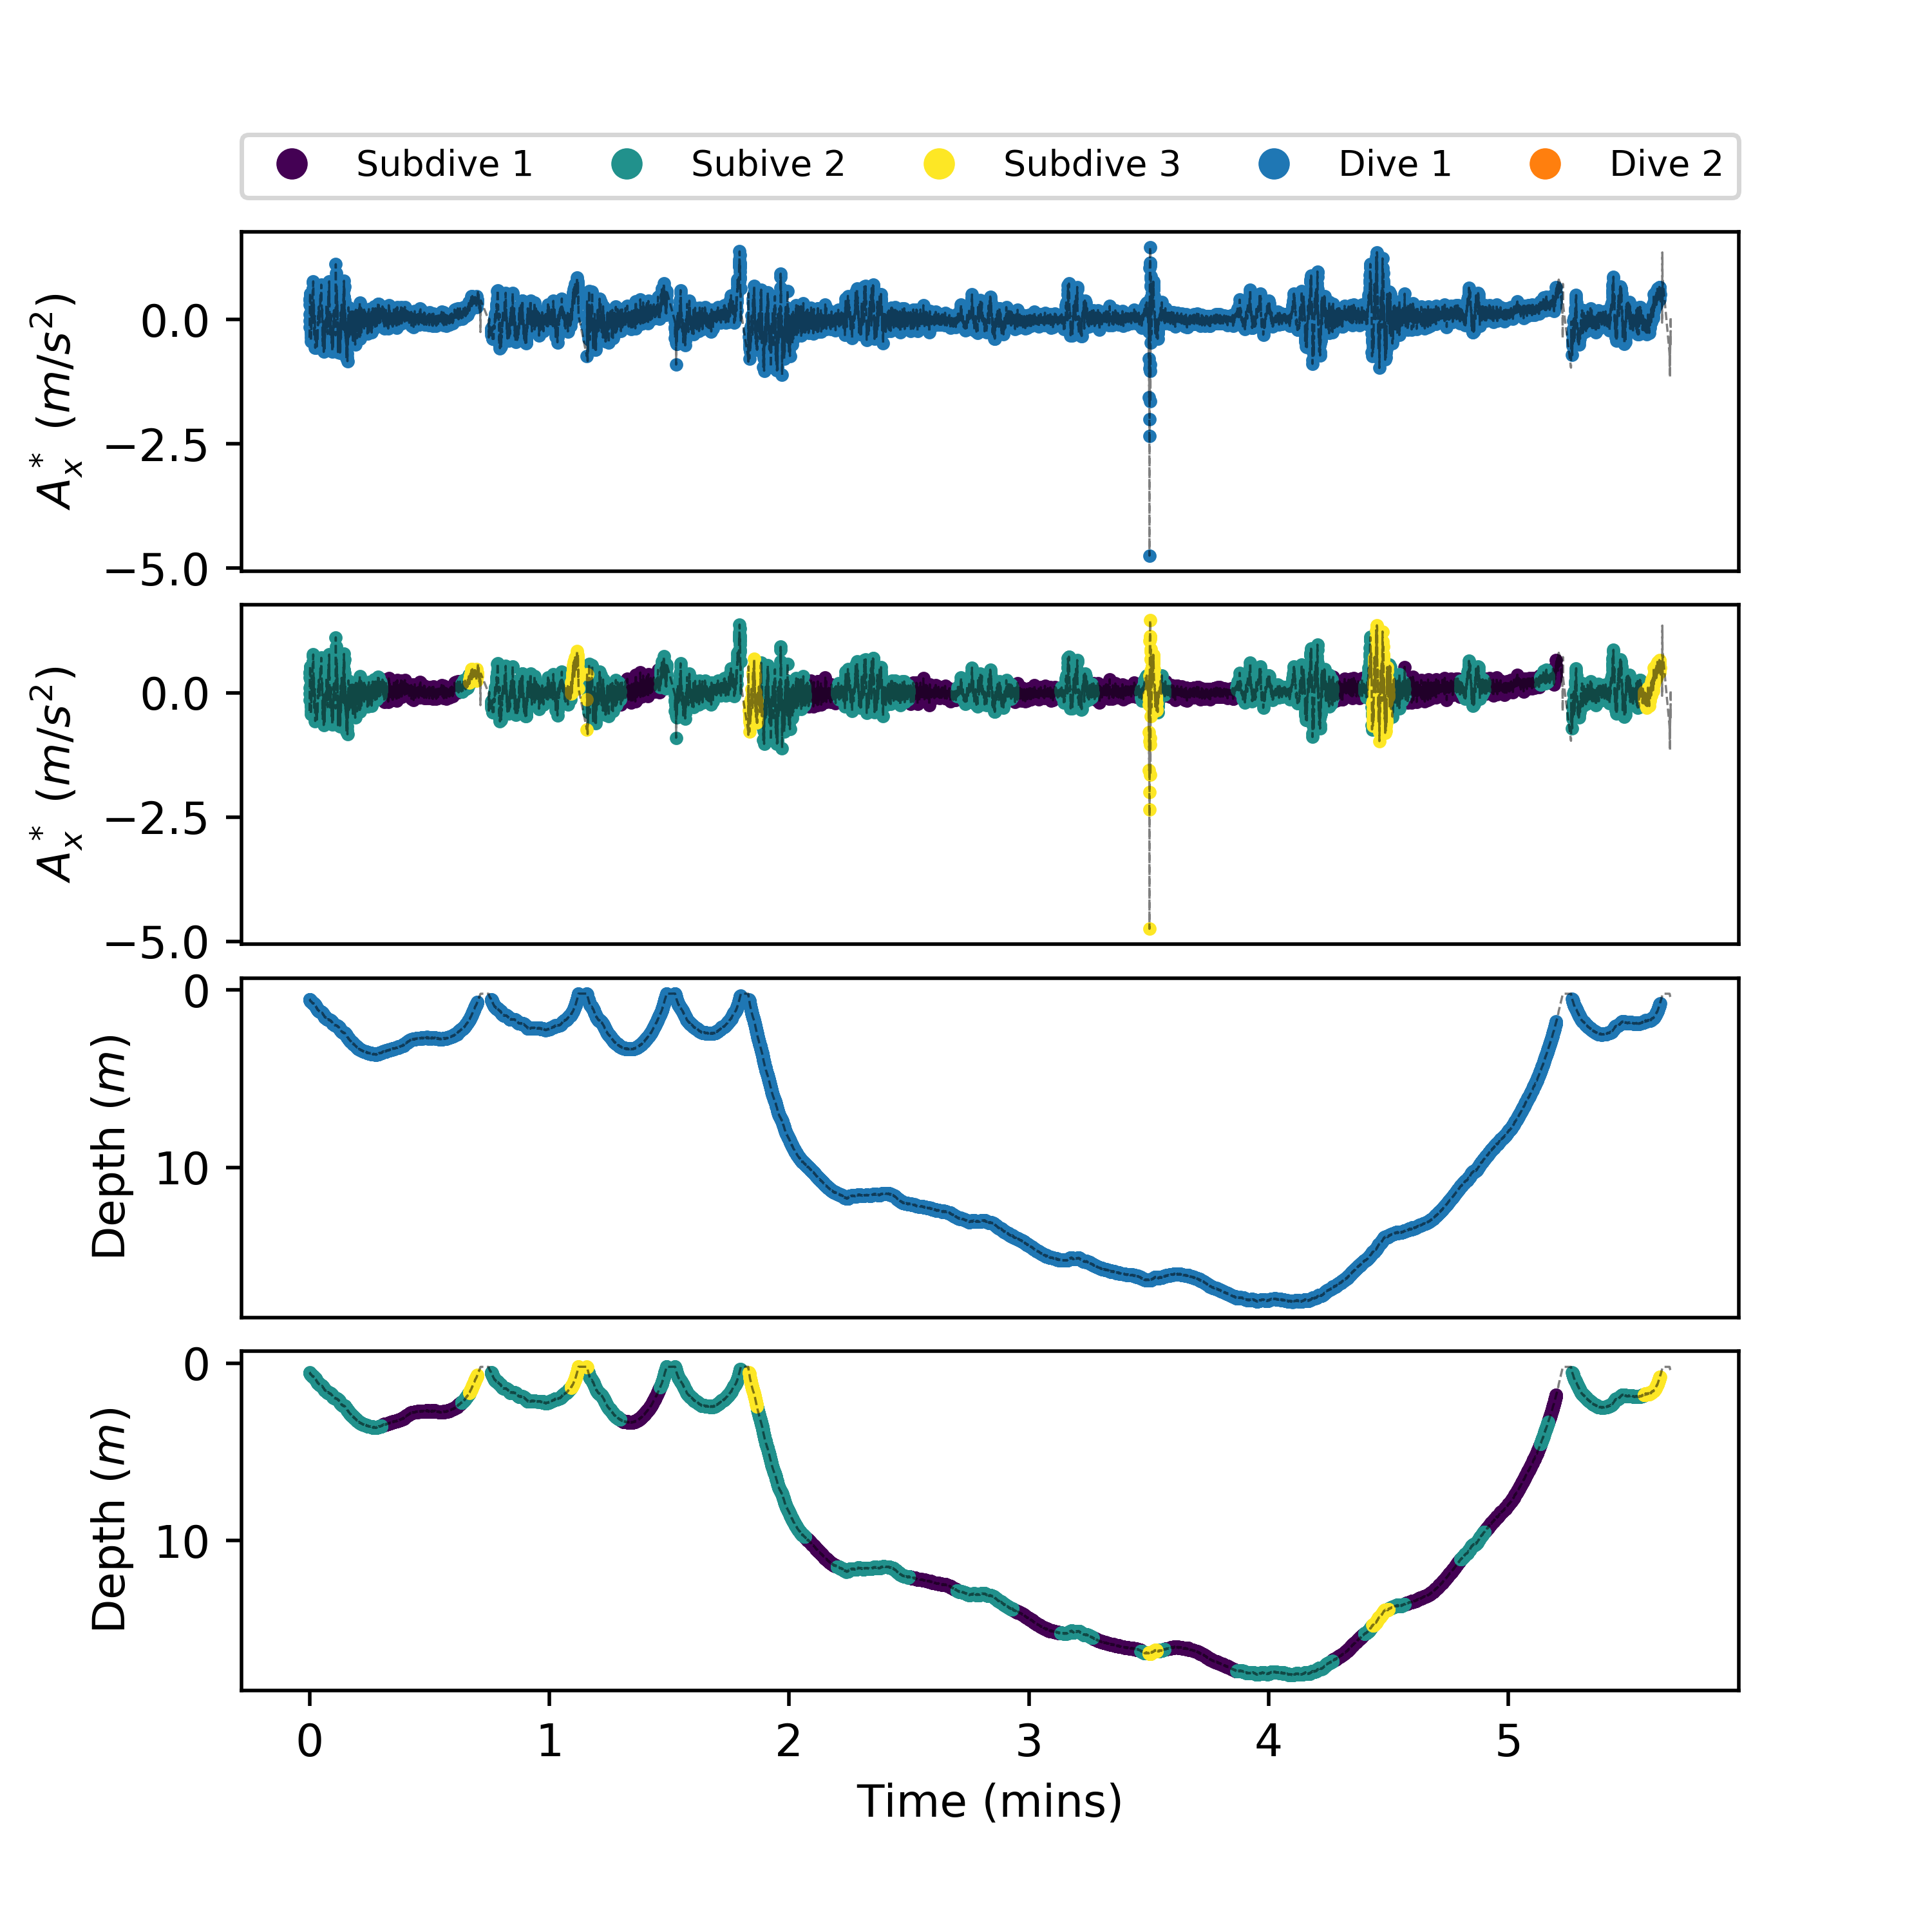
\includegraphics[width=6in]{../Plots/CarHMM_decoded_dives.png}
        \end{center}
        
        \noindent Figure \arabic{fignum}: The $x$-component of acceleration $\left(y^*_{t,t^*}\right)_x$ and dive profile of a northern resident killer whale for dives $t = 160,161,162,163,164,$ and $165$. The line colour of the first and third panels corresponds to the estimated dive type while the line colour of the second and fourth panels corresponds to the estimated subdive state. Both the dive types and subdive states are estimated by fitting the CarHMM-DFT to the data.
        \addtocounter{fignum}{1}
        
        \begin{center}
        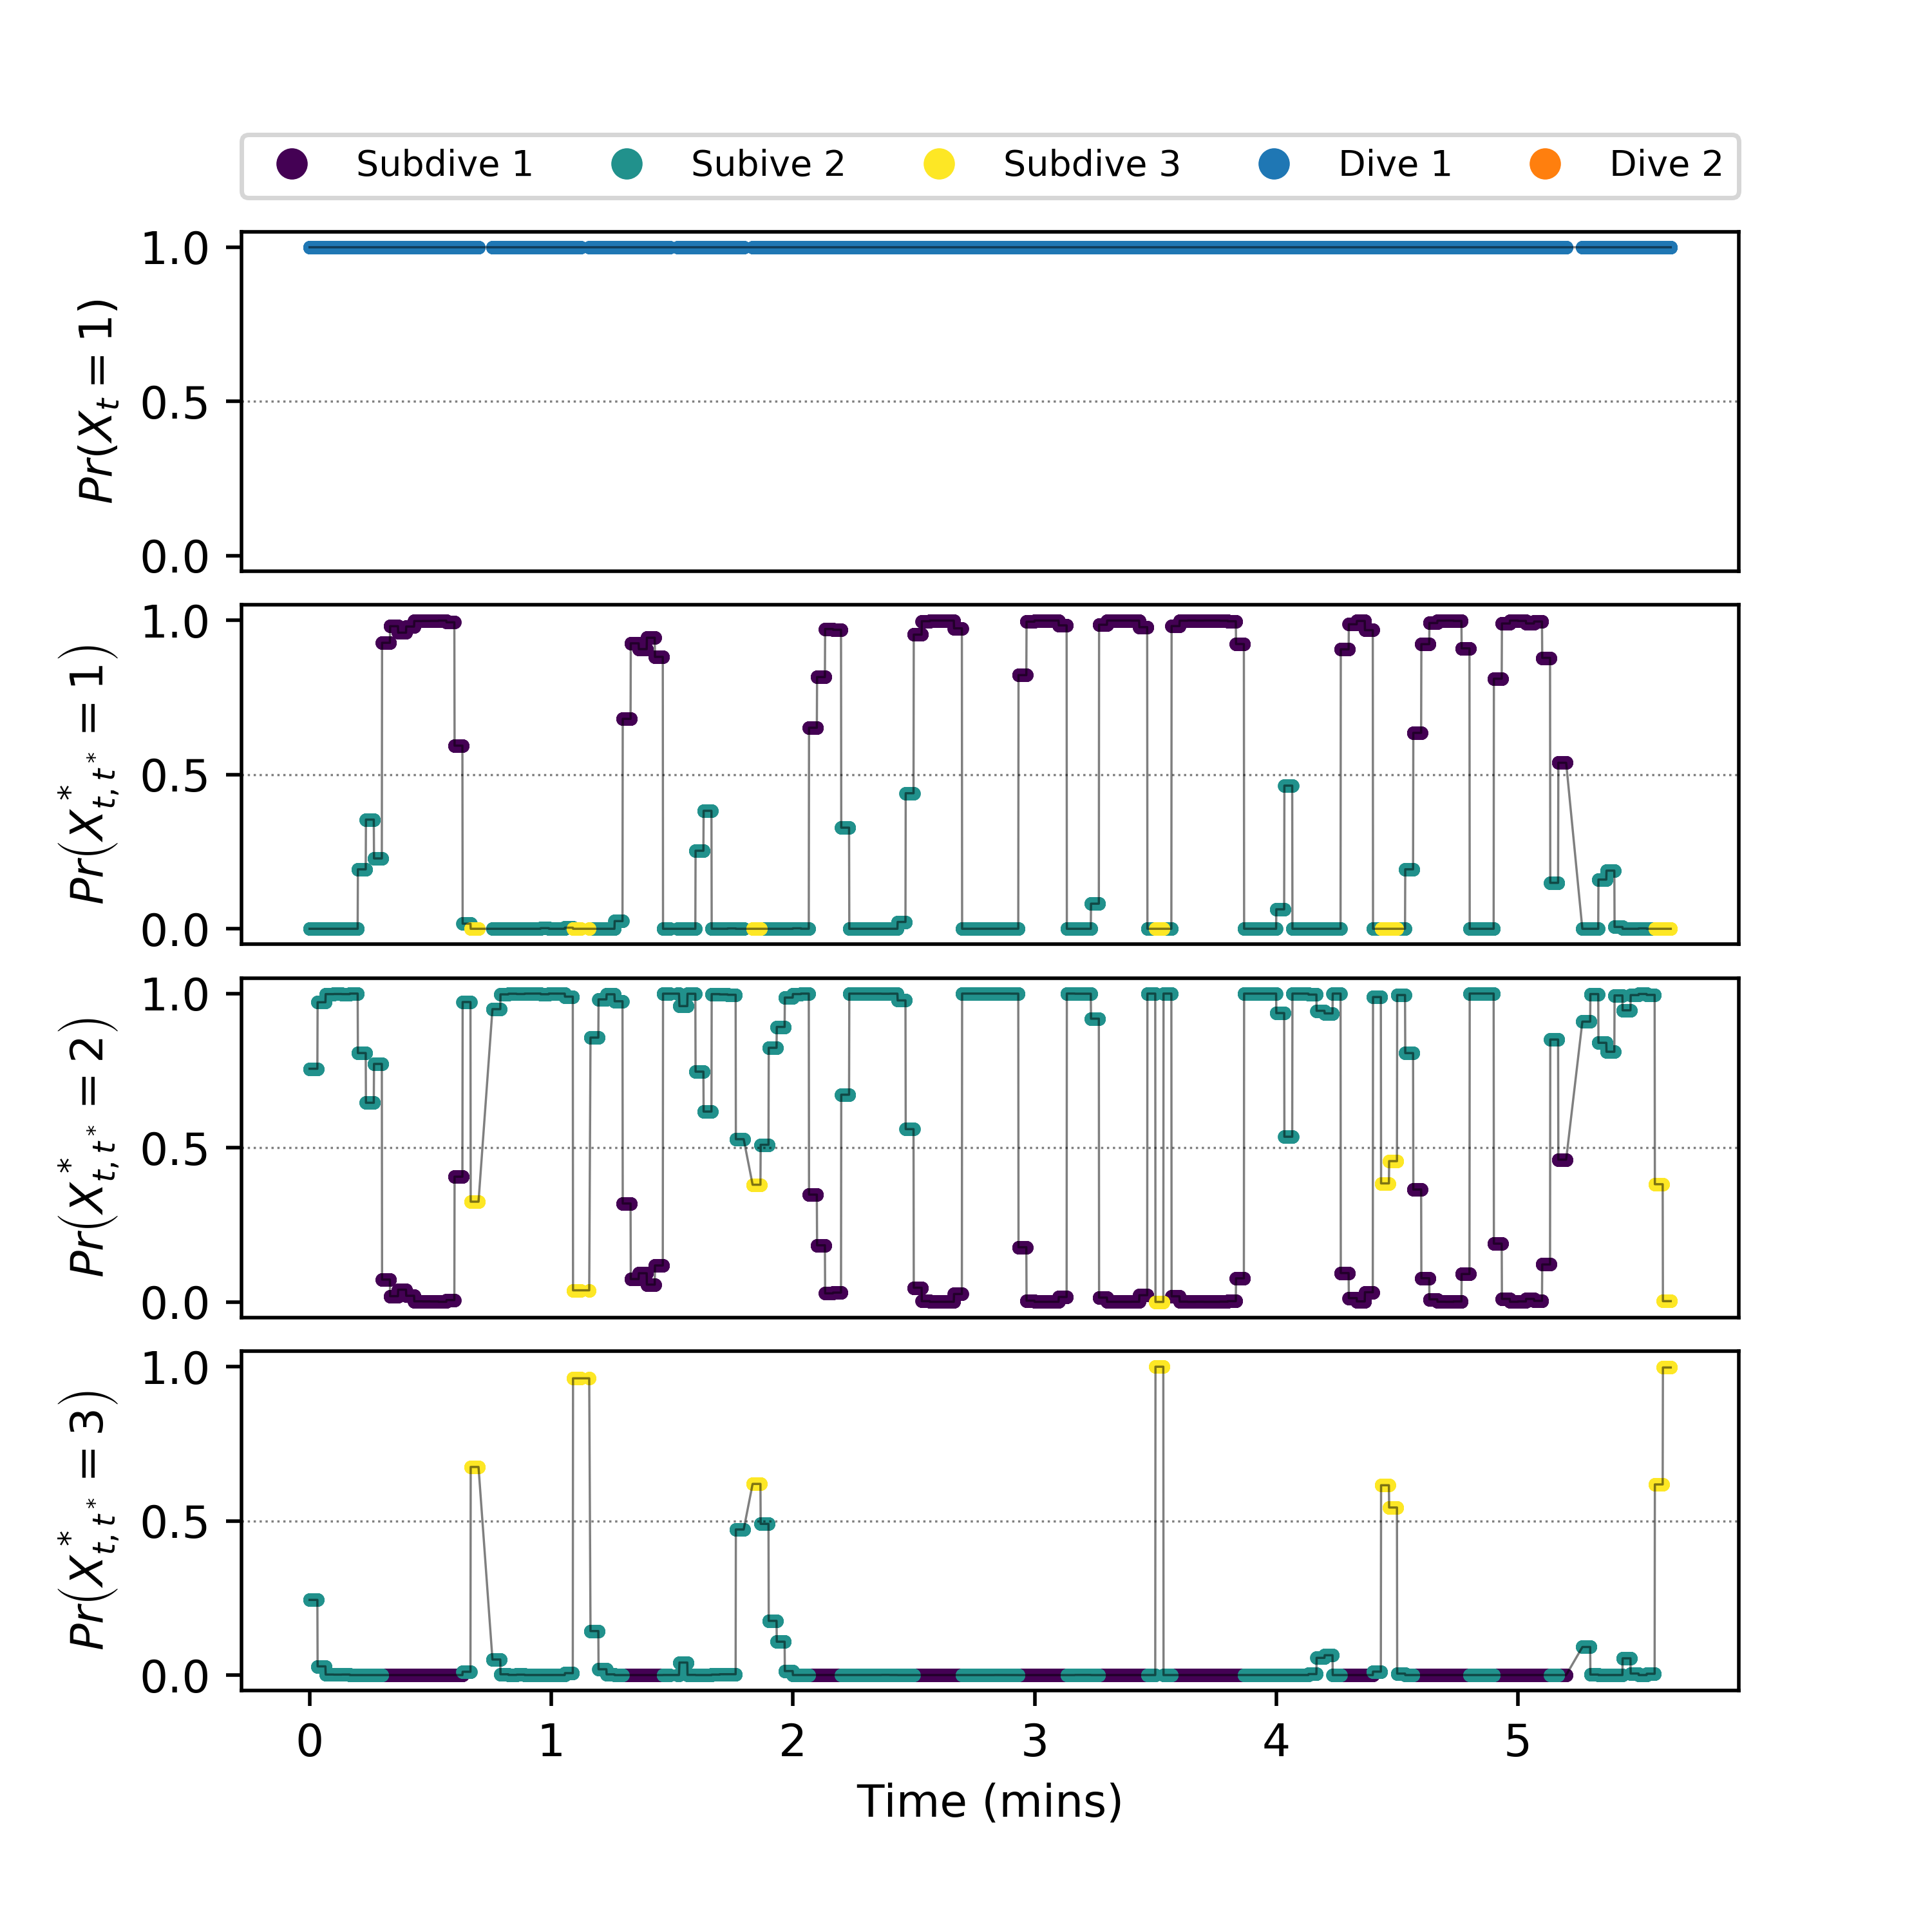
\includegraphics[width=6in]{../Plots/CarHMM_decoded_states.png}
        \end{center}
        
        \noindent Figure \arabic{fignum}: The probability that each dive is a particular type or that the whale is in a particular subdive state, given the fitted model. This is shown for dives $t = 160,161,162,163,164,$ and $165$. The line colour of the first panel corresponds to the estimated dive type while the line colour of the last three panels corresponds to the estimated subdive state. Both the dive types and subdive states are estimated by fitting the CarHHMM-DFT to the data.
        \addtocounter{fignum}{1}
        
    \newpage
    \subsection{Model checking - dive duration ($Y_t$)}
    
        \subsubsection{CarHHMM-DFT}
        
        \begin{center}
        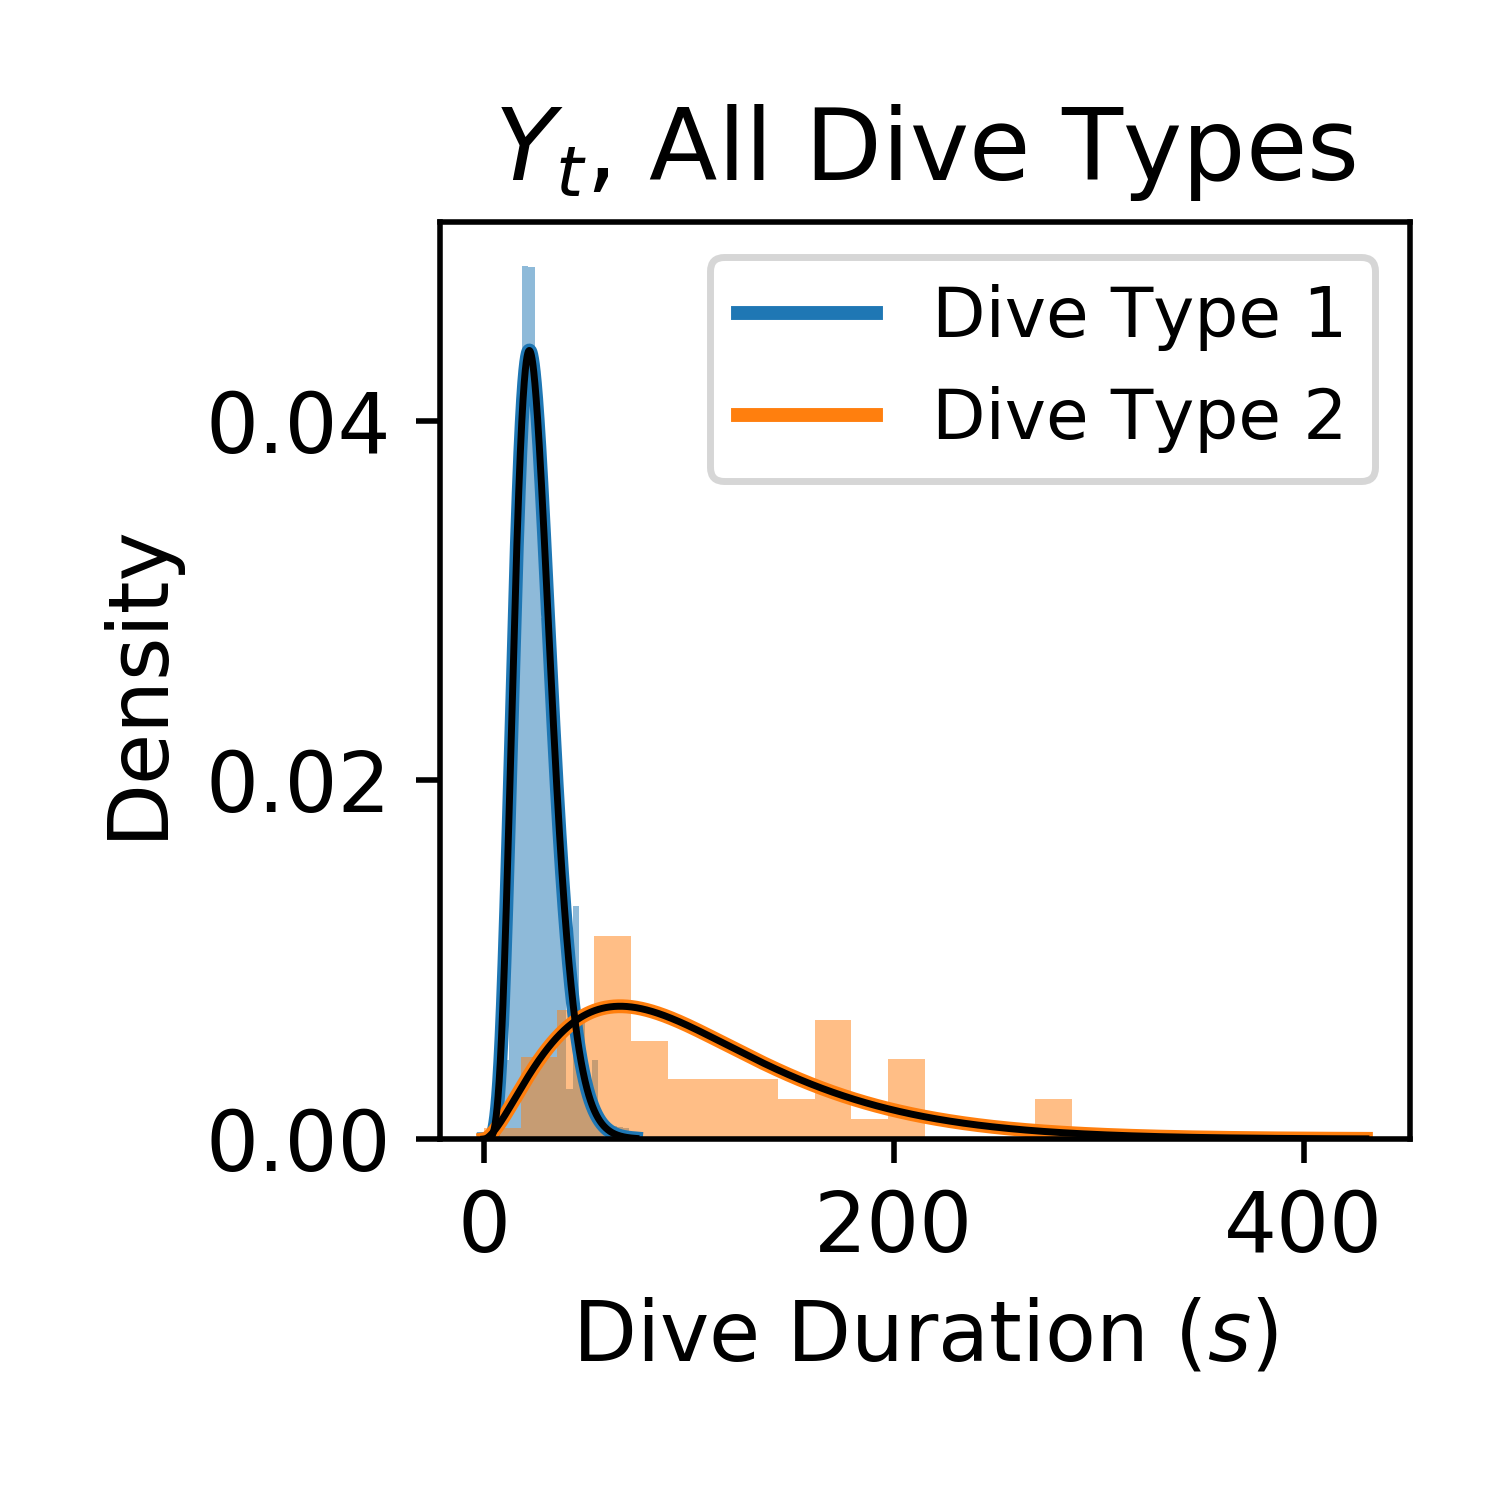
\includegraphics[width=2.25in]{../Plots/CarHHMM2_empirical_hist_dive_duration.png}
        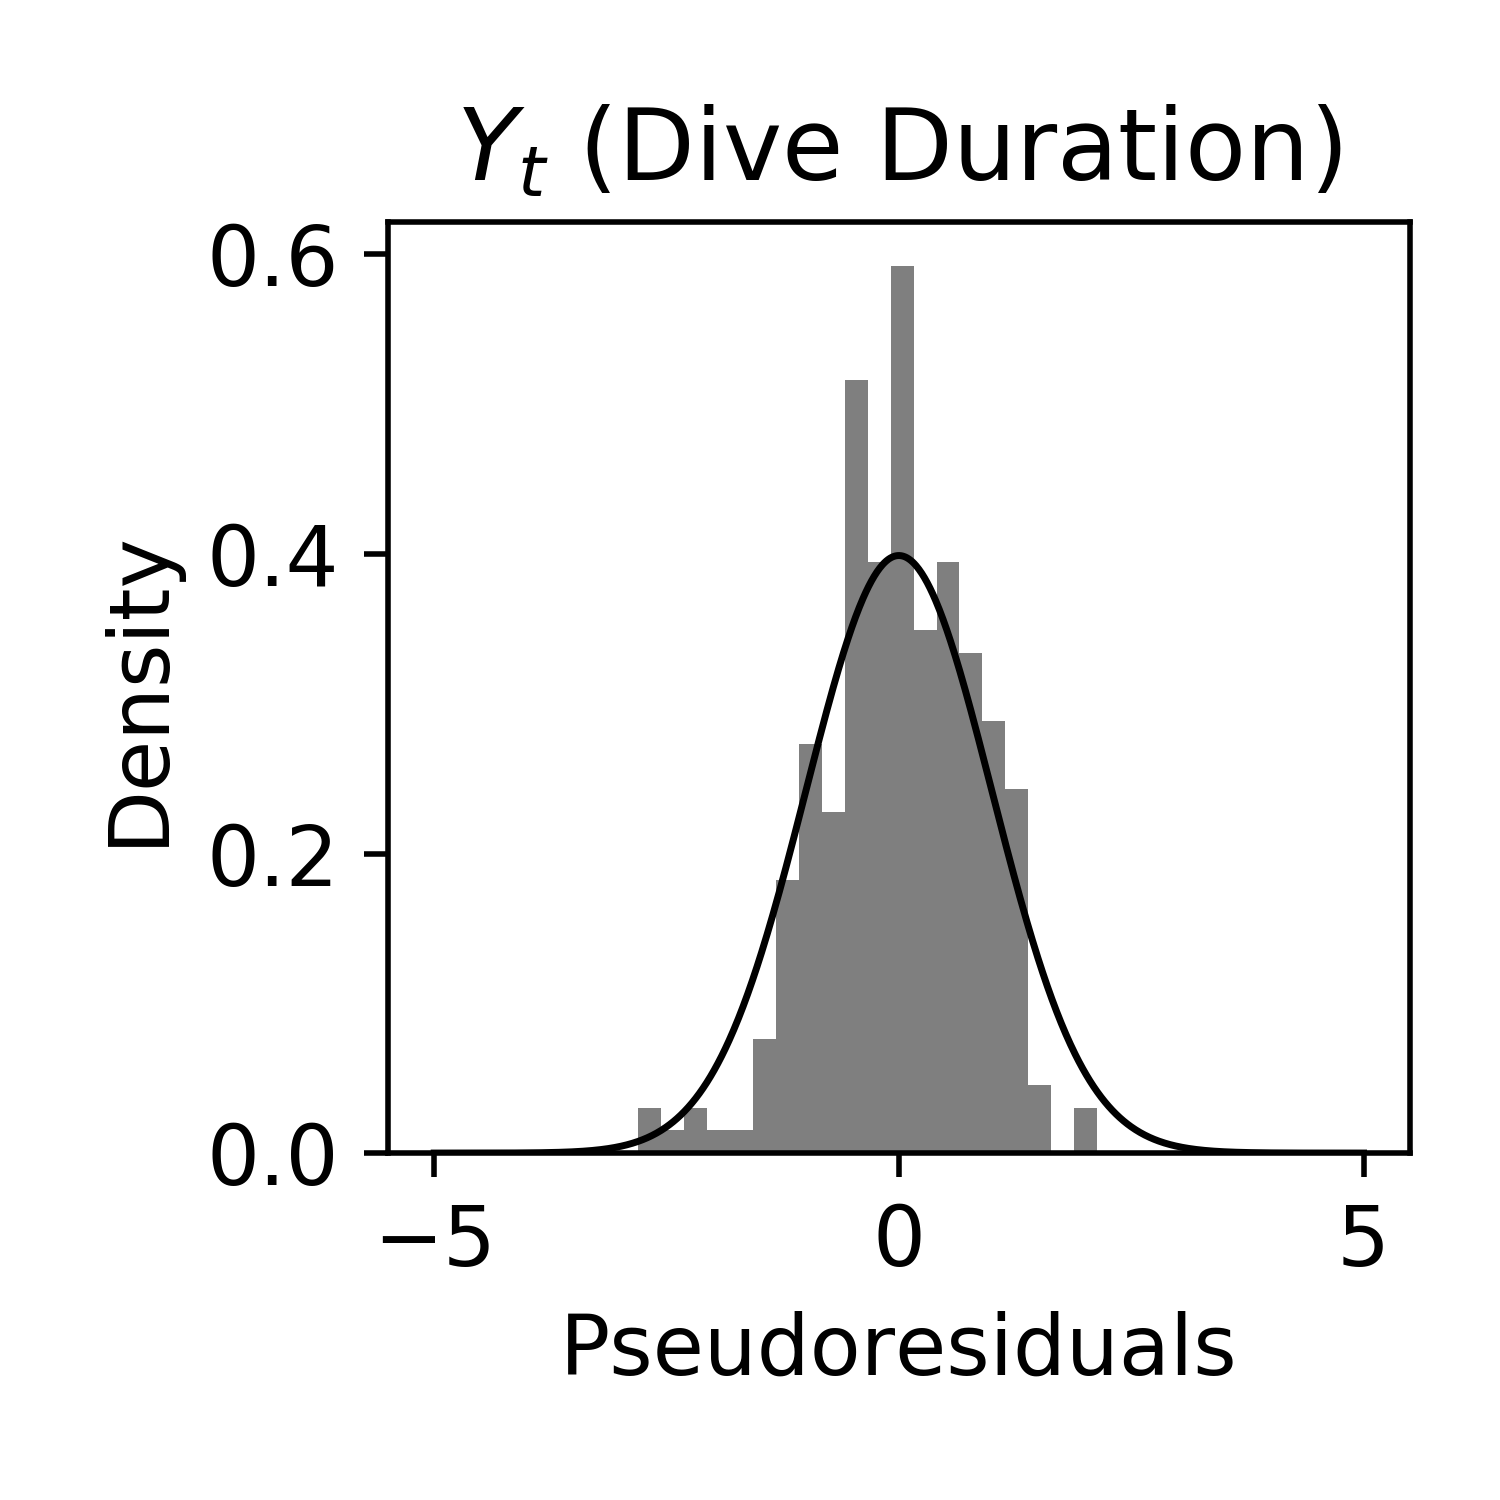
\includegraphics[width=2.25in]{../Plots/CarHHMM2_psedoresids_Dive_Duration.png}
        \end{center}
        
        \noindent Figure \arabic{fignum}: Empirical histogram (left) and psuedoresiduals (right) of dive duration ($Y_{t}$) plotted over the learned emission distributions and a standard normal density, respectively. Both plots are generated using the fitted CarHHMM-DFT and the killer whale case study data.
        \addtocounter{fignum}{1}
        
        \subsubsection{HHMM-DFT}
        
        \begin{center}
        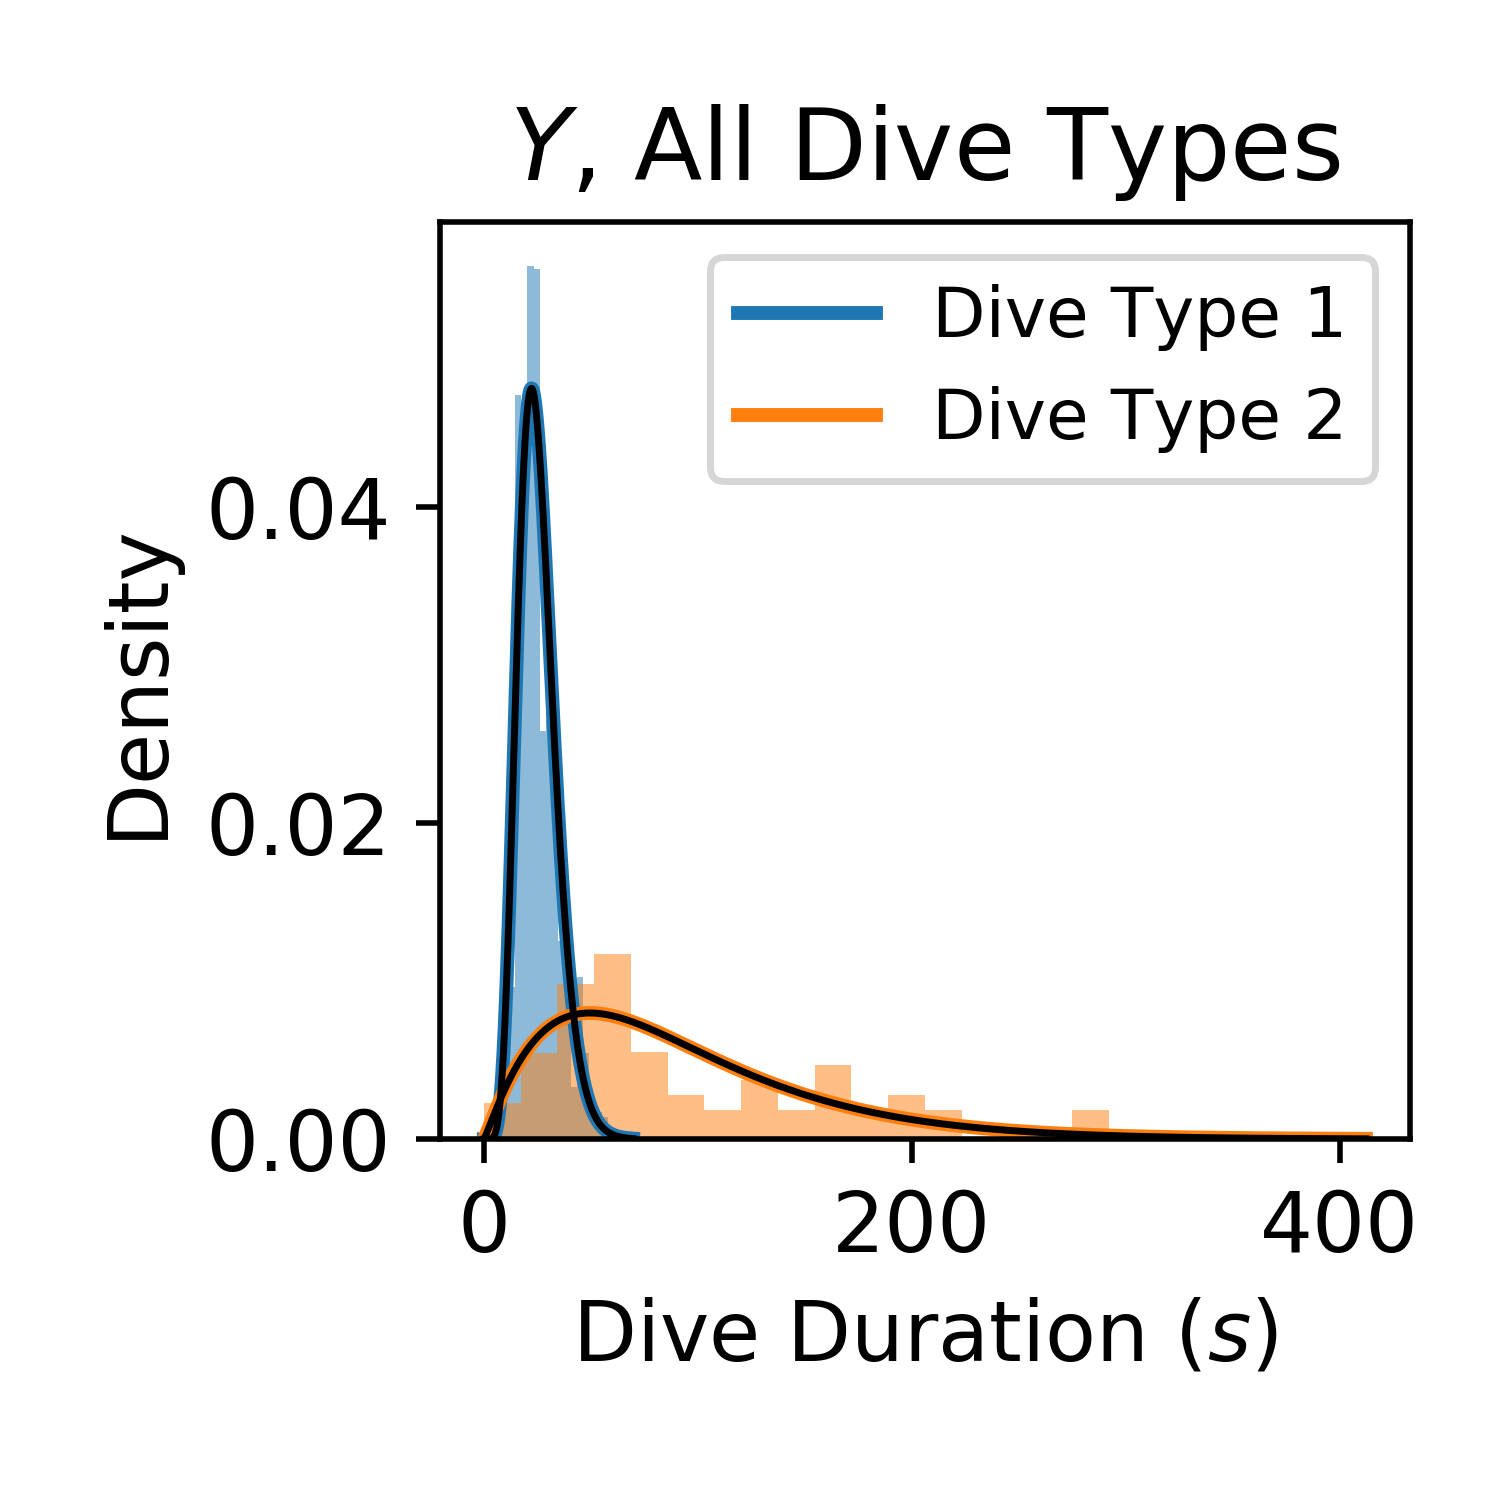
\includegraphics[width=2.25in]{../Plots/HHMM_empirical_hist_dive_duration.png}
        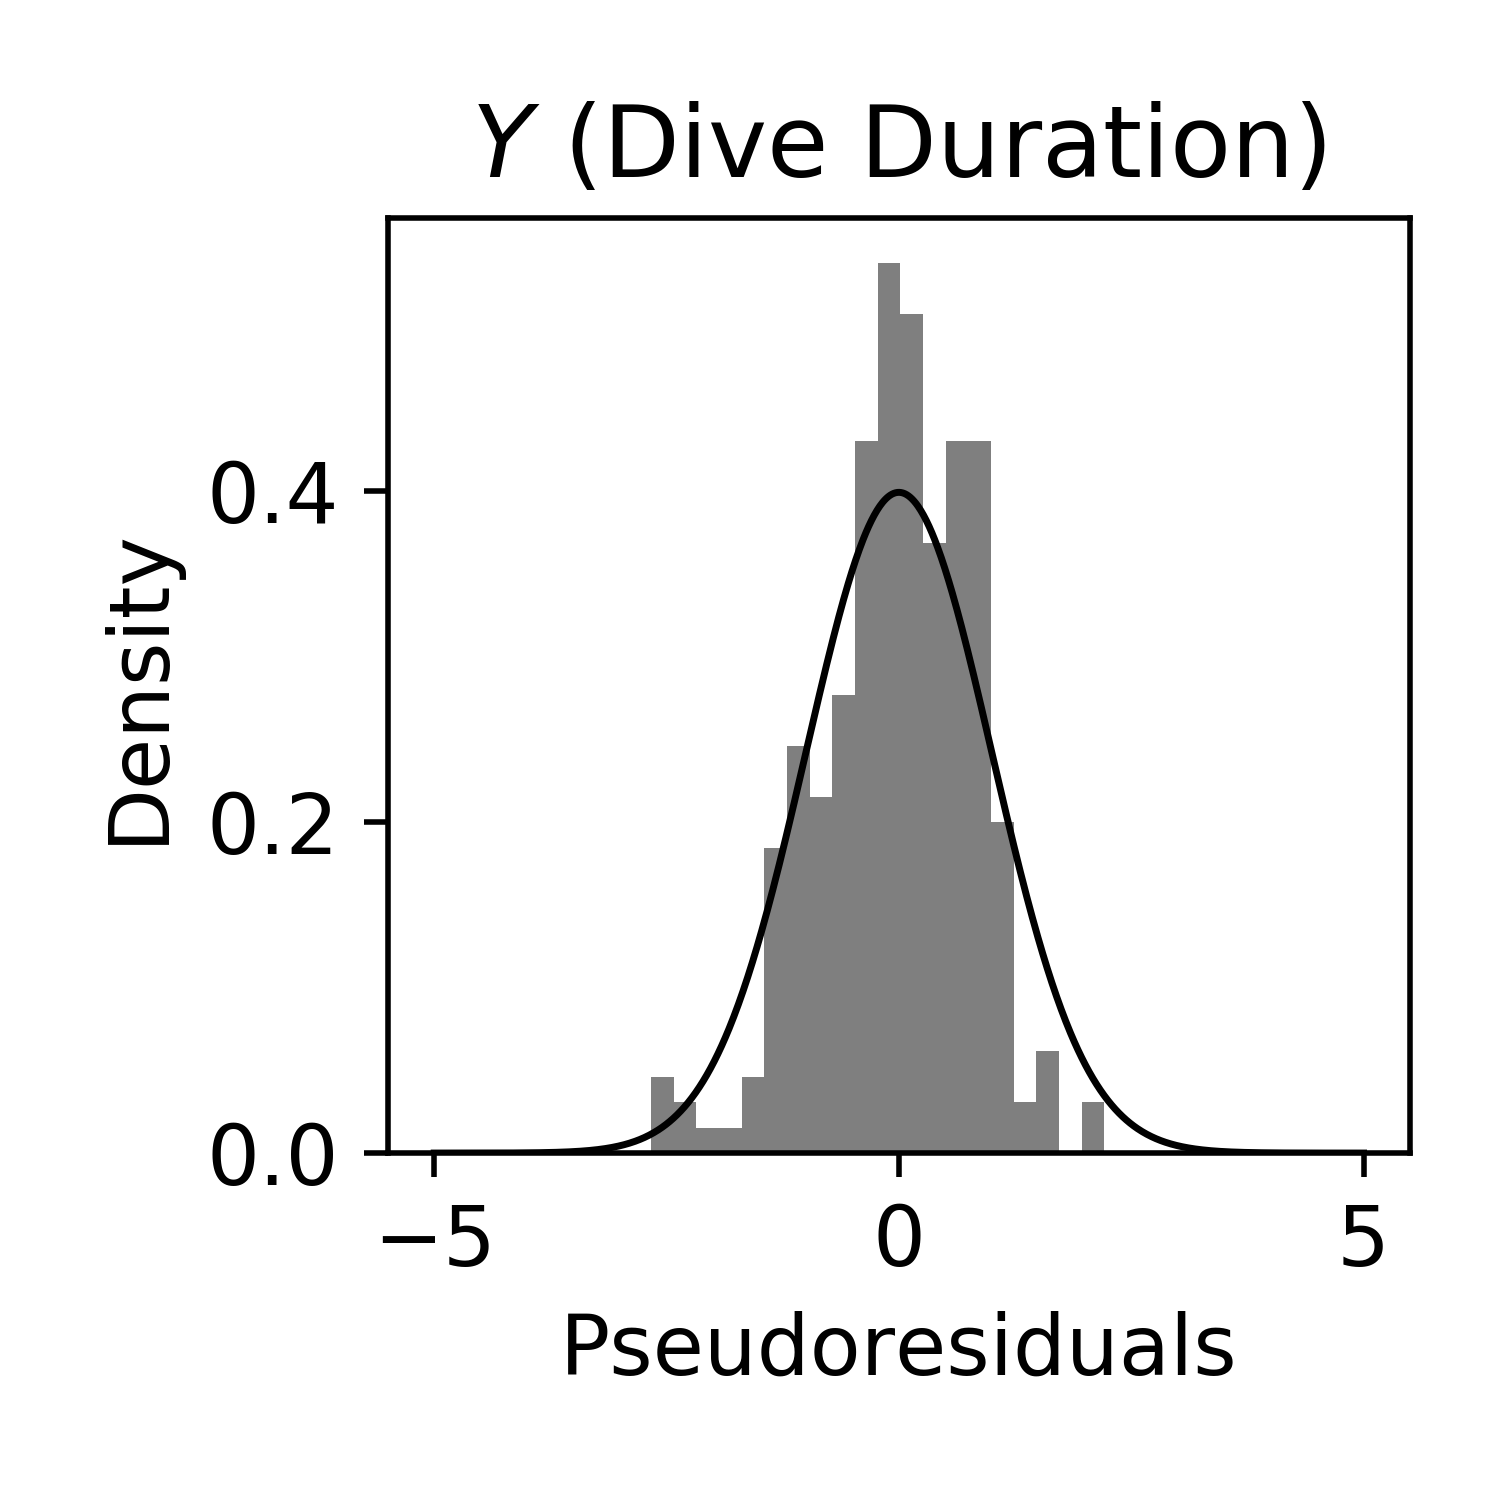
\includegraphics[width=2.25in]{../Plots/HHMM_psedoresids_Dive_Duration.png}
        \end{center}
        
        \noindent Figure \arabic{fignum}: Empirical histogram (left) and psuedoresiduals (right) of dive duration ($Y_{t}$) plotted over the learned emission distributions and a standard normal density, respectively. Both plots are generated using the fitted HHMM-DFT and the killer whale case study data.
        \addtocounter{fignum}{1}
        
        \subsubsection{CarHHMM}
        
        \begin{center}
        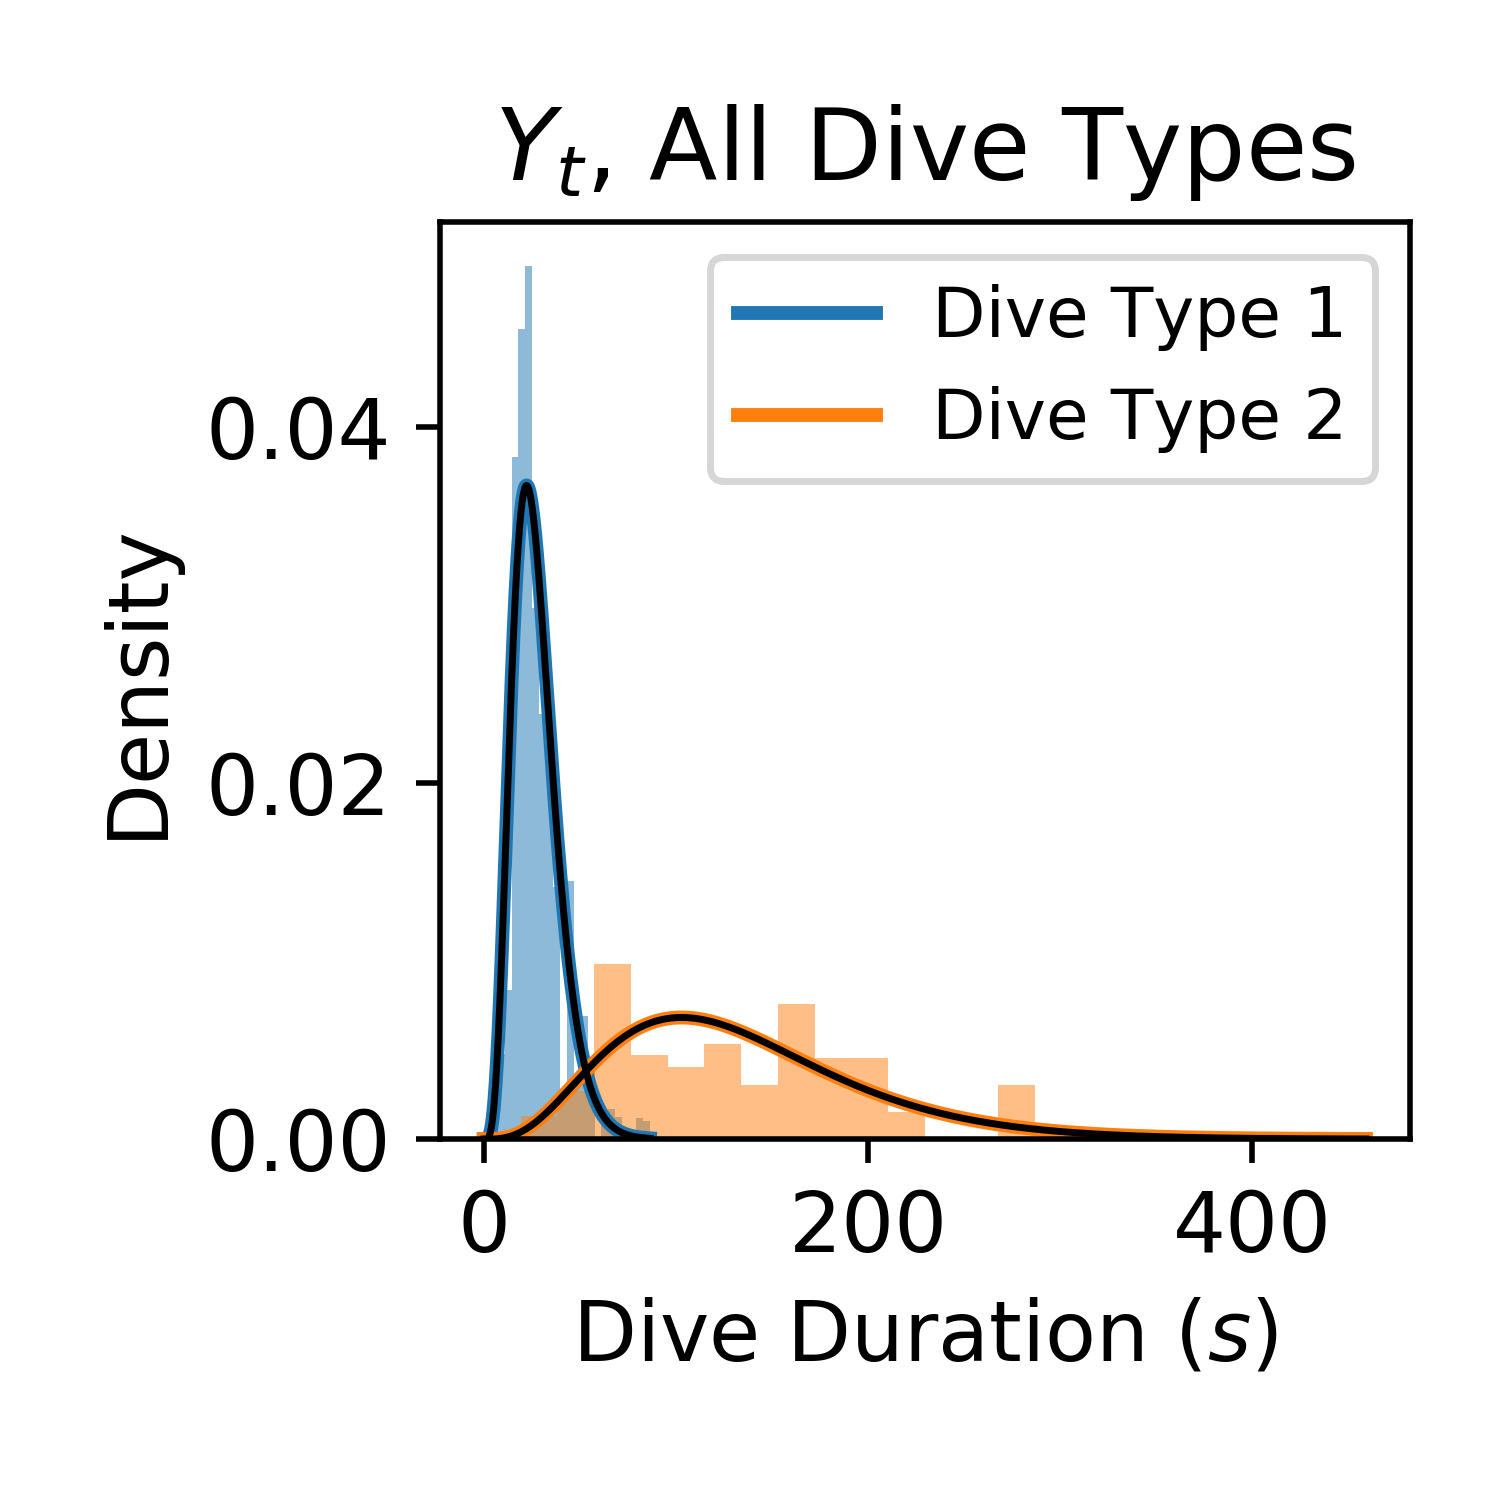
\includegraphics[width=2.25in]{../Plots/CarHHMM1_empirical_hist_dive_duration.png}
        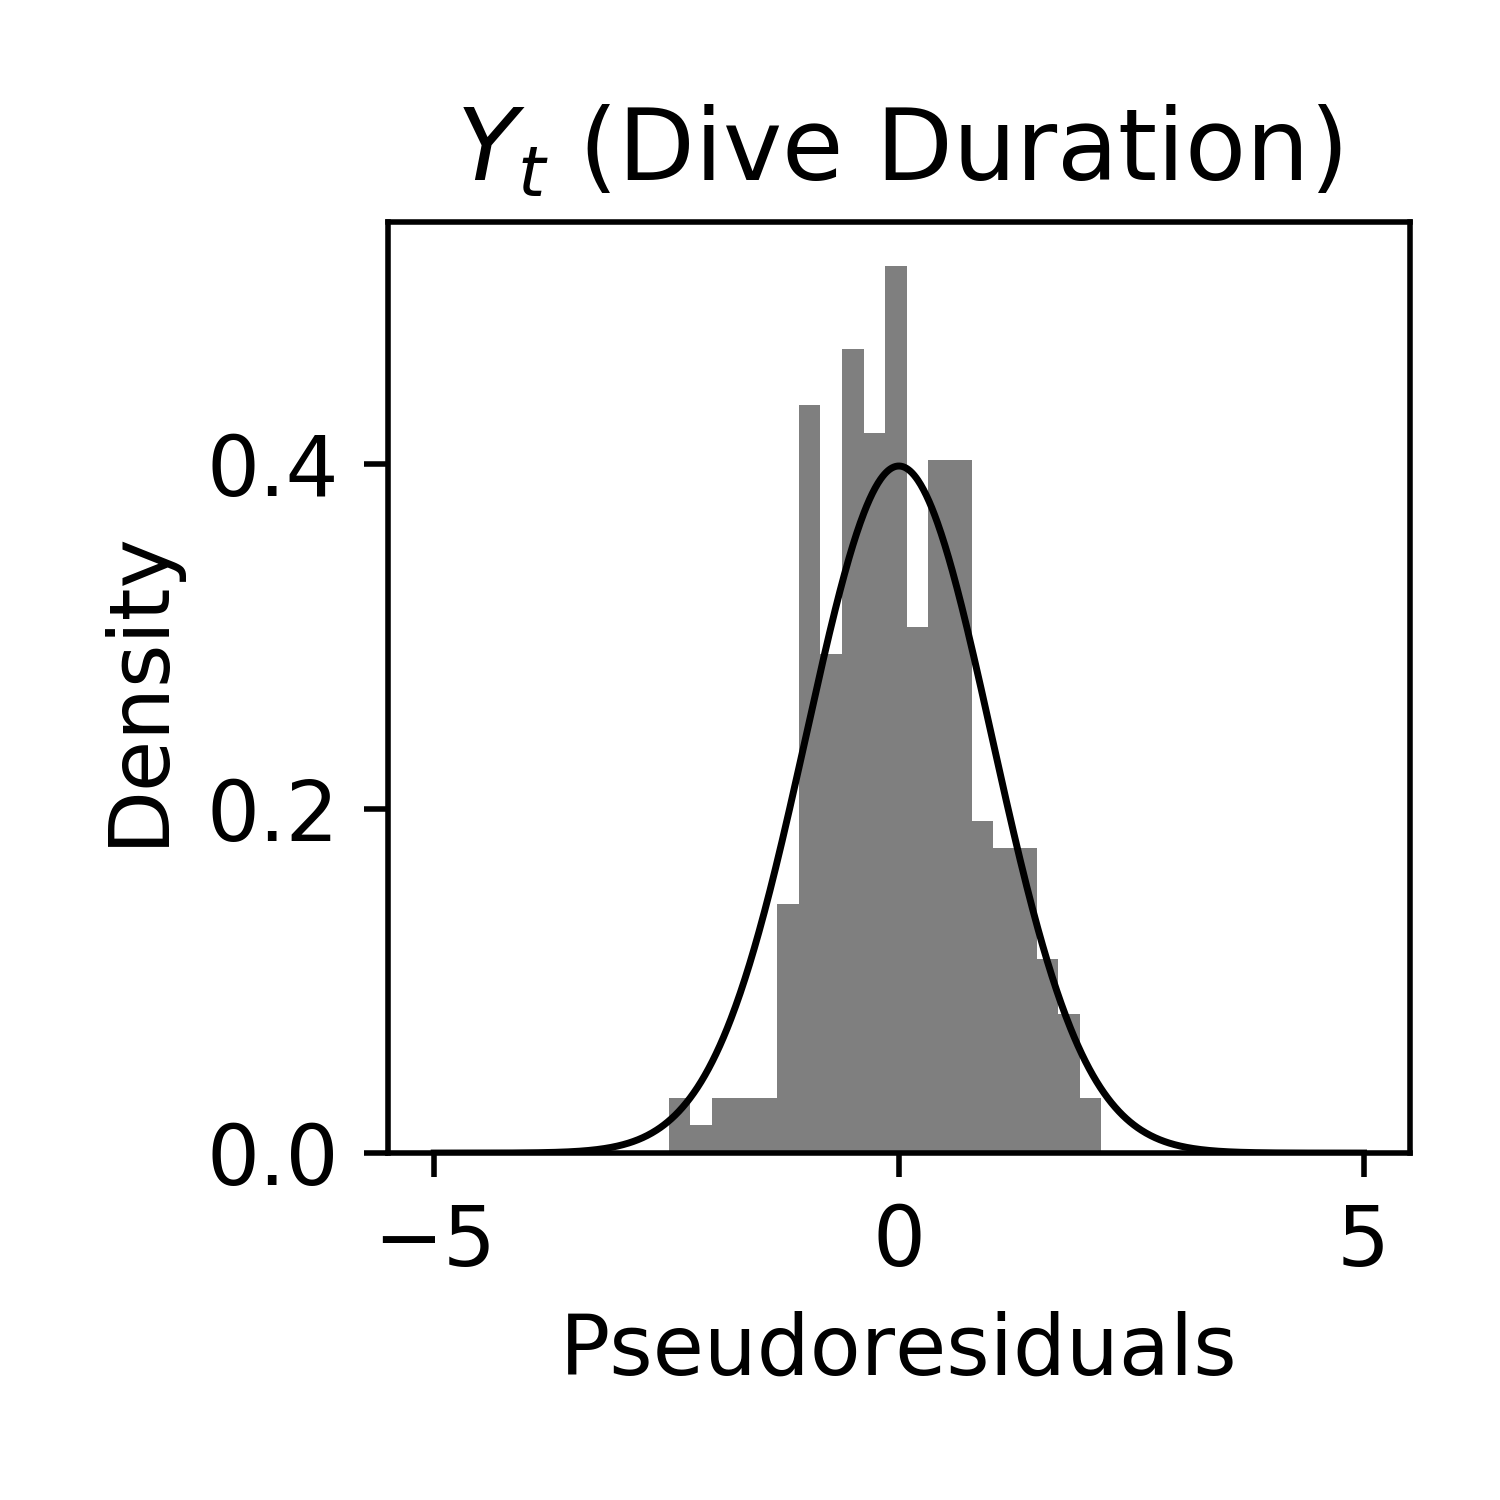
\includegraphics[width=2.25in]{../Plots/CarHHMM1_psedoresids_Dive_Duration.png}
        \end{center}
        
        \noindent Figure \arabic{fignum}: Empirical histogram (left) and psuedoresiduals (right) of dive duration ($Y_{t}$) plotted over the learned emission distributions and a standard normal density, respectively. Both plots are generated using the fitted CarHHMM-DFT and the killer whale case study data.
        \addtocounter{fignum}{1}
        
        \subsubsection{CarHMM-DFT}
        
        \begin{center}
        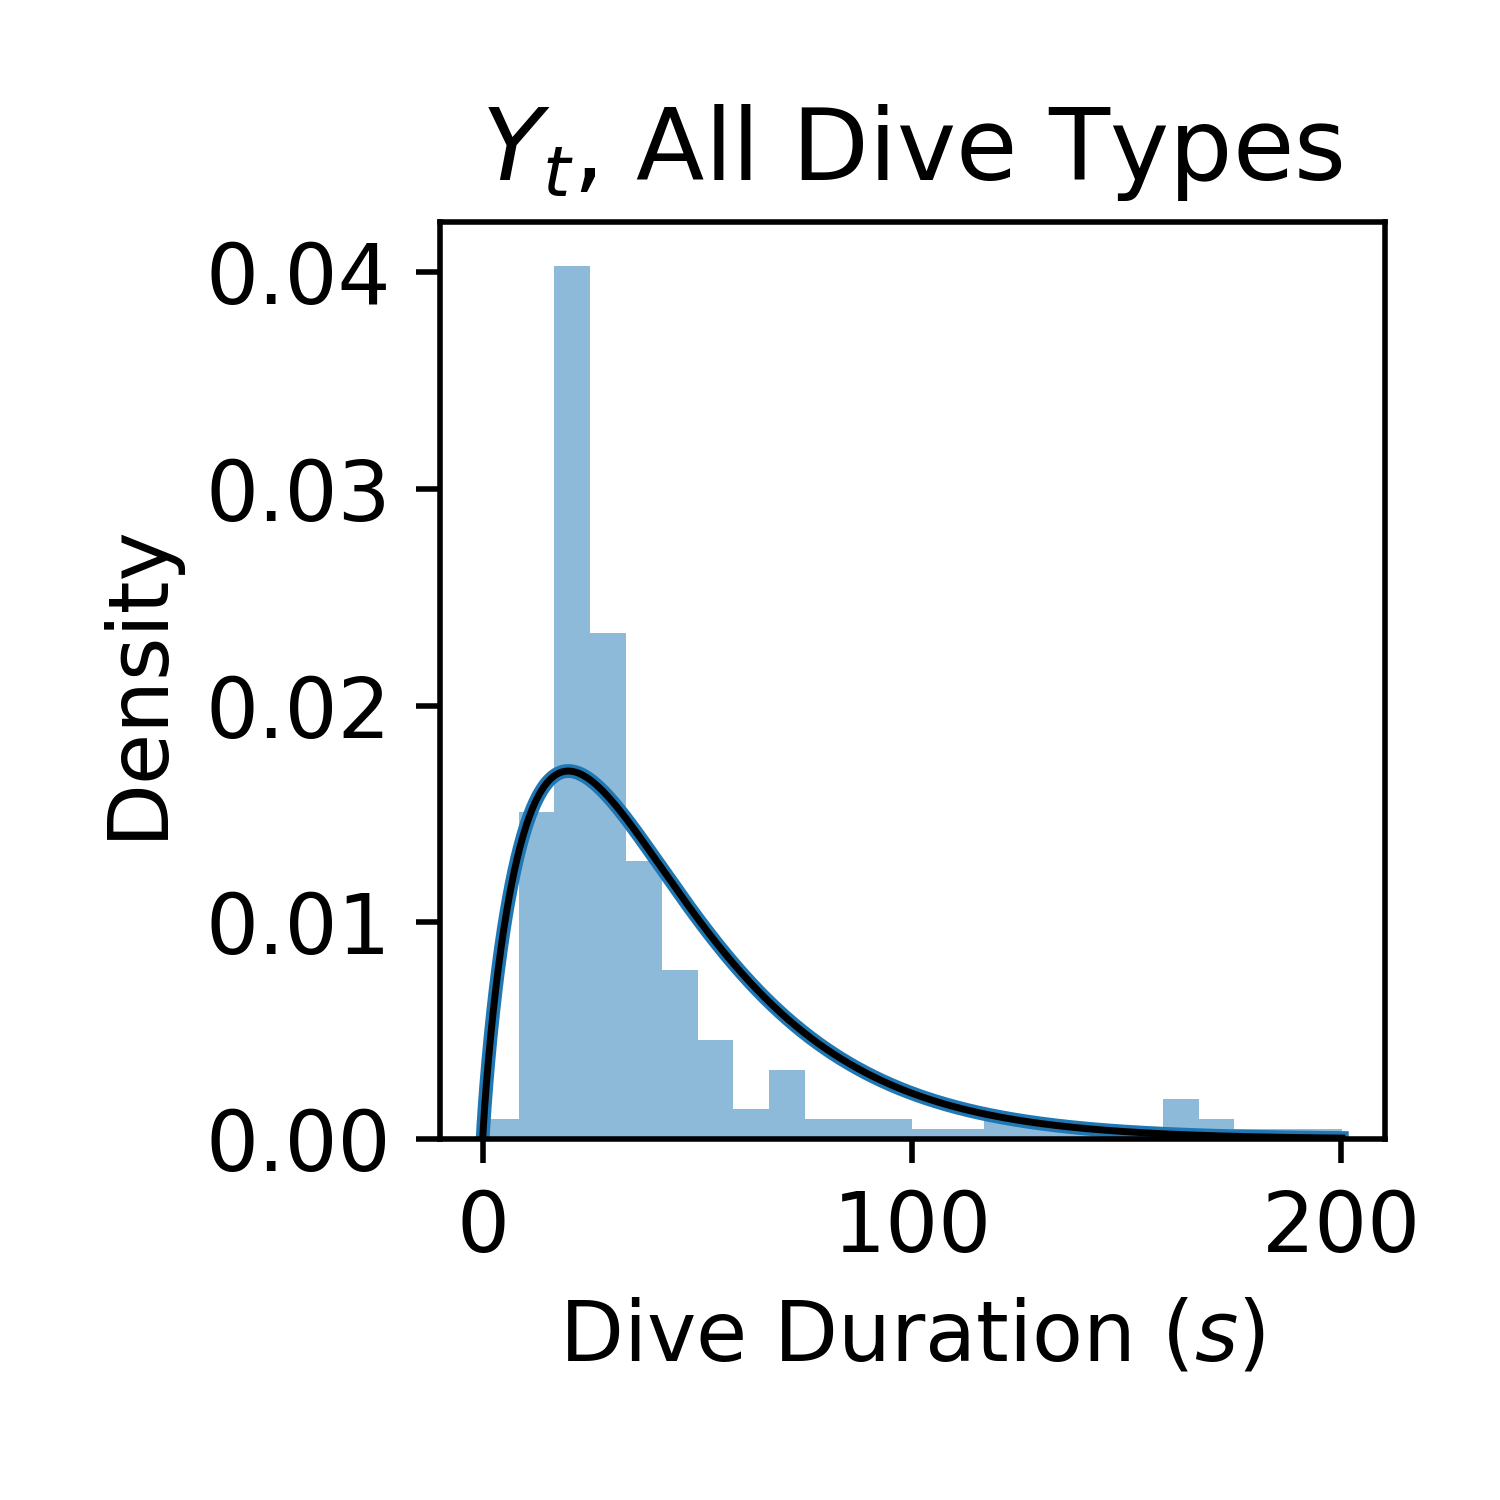
\includegraphics[width=2.25in]{../Plots/CarHMM_empirical_hist_dive_duration.png}
        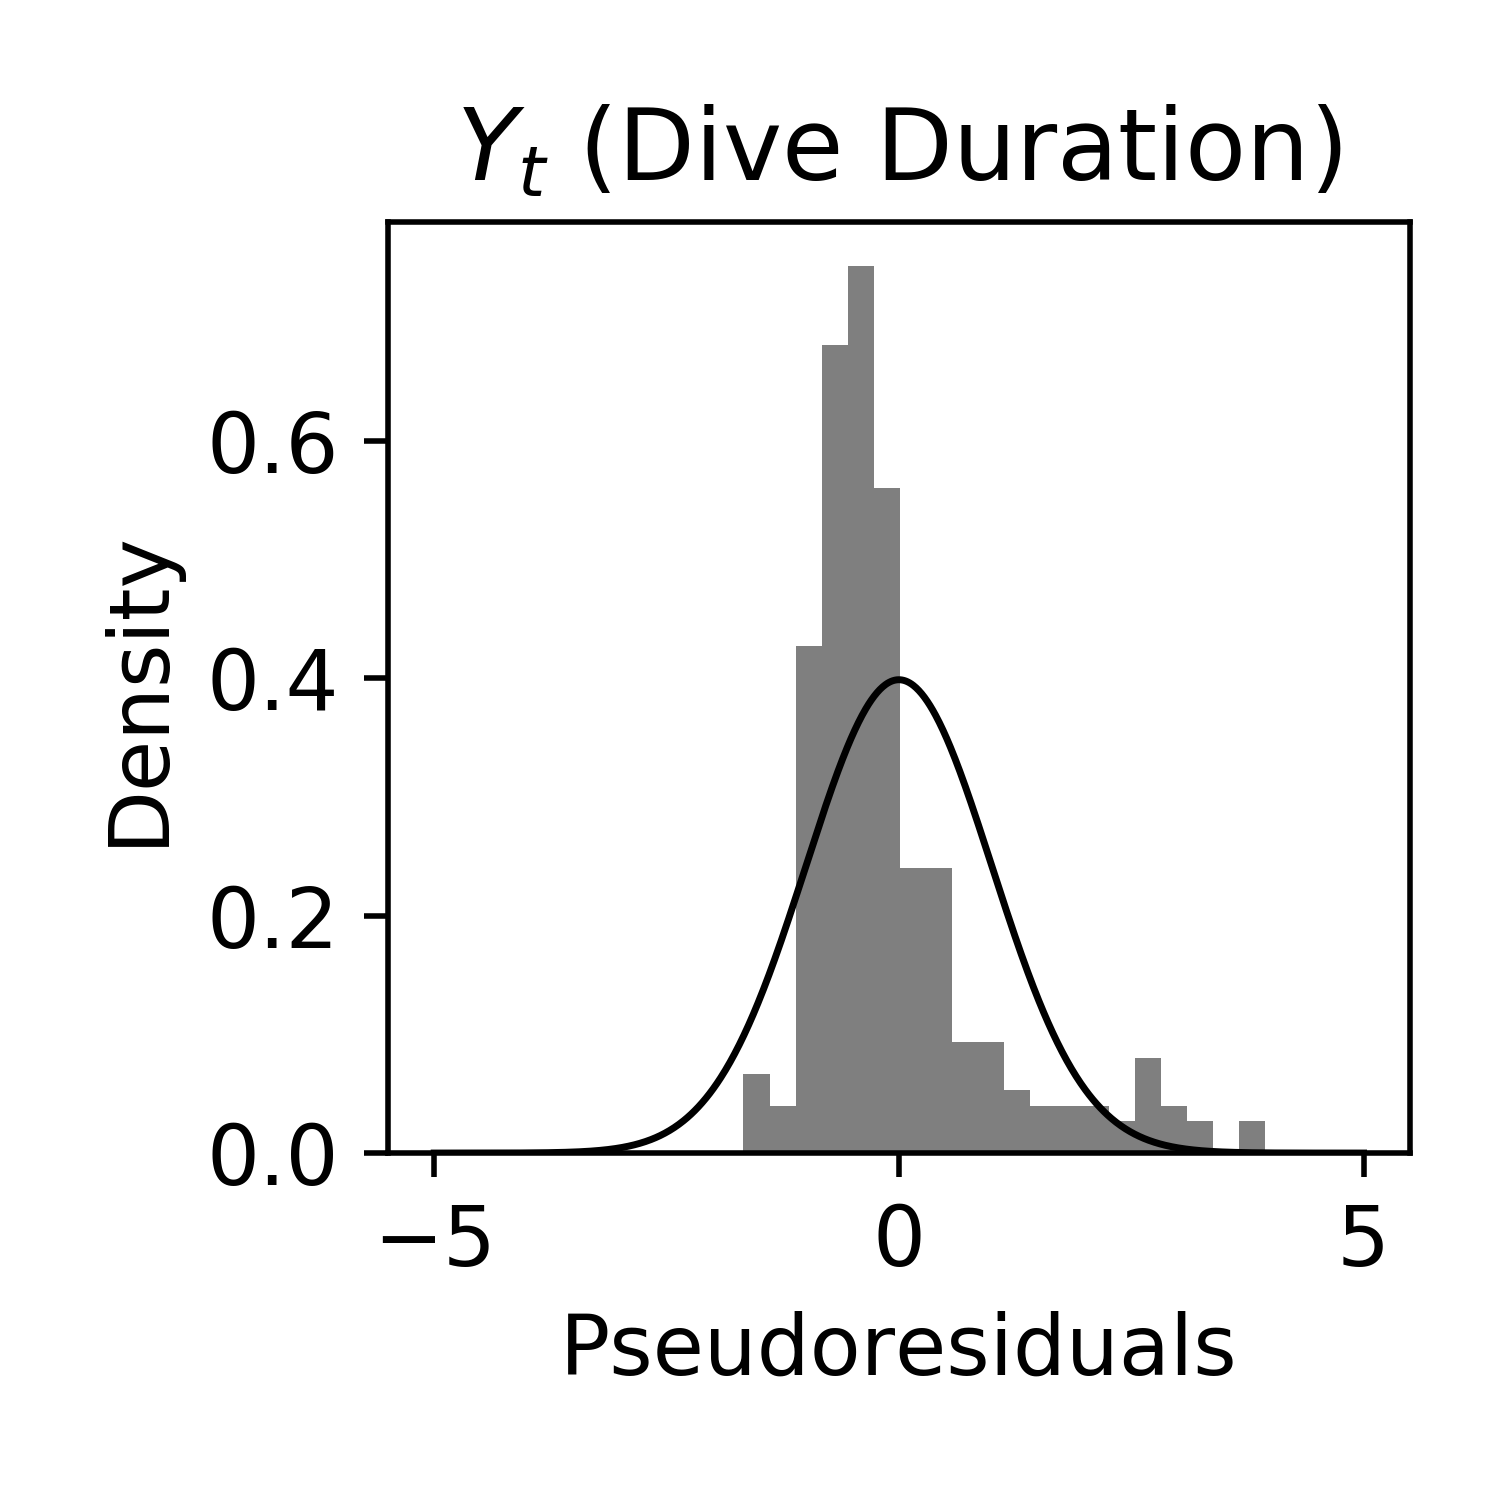
\includegraphics[width=2.25in]{../Plots/CarHMM_psedoresids_Dive_Duration.png}
        \end{center}
        
        \noindent Figure \arabic{fignum}: Empirical histogram (left) and psuedoresiduals (right) of dive duration ($Y_{t}$) plotted over the learned emission distribution (left) and a standard normal density (right), respectively. Both plots are generated using the fitted CarHMM-DFT and the killer whale case study data.
        \addtocounter{fignum}{1}
        
    \newpage
    \subsection{Model checking - acceleration ($\Zone_{t,t^*}$)}
        
        \subsubsection{CarHHMM-DFT}
        
        \begin{center}
        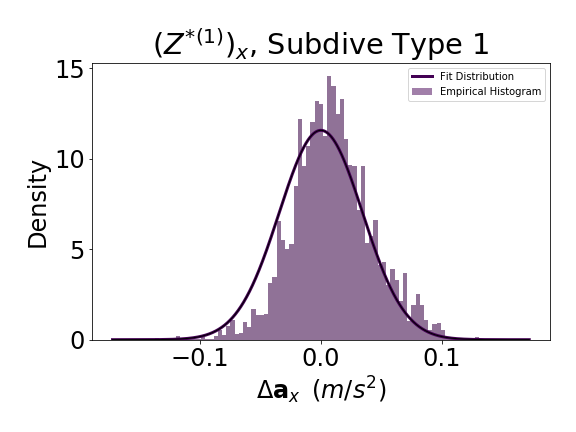
\includegraphics[width=1.75in]{../Plots/CarHHMM2_empirical_hist_Ax_0.png}
        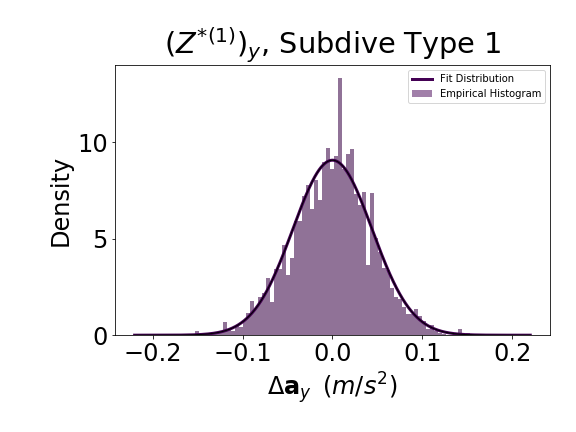
\includegraphics[width=1.75in]{../Plots/CarHHMM2_empirical_hist_Ay_0.png}
        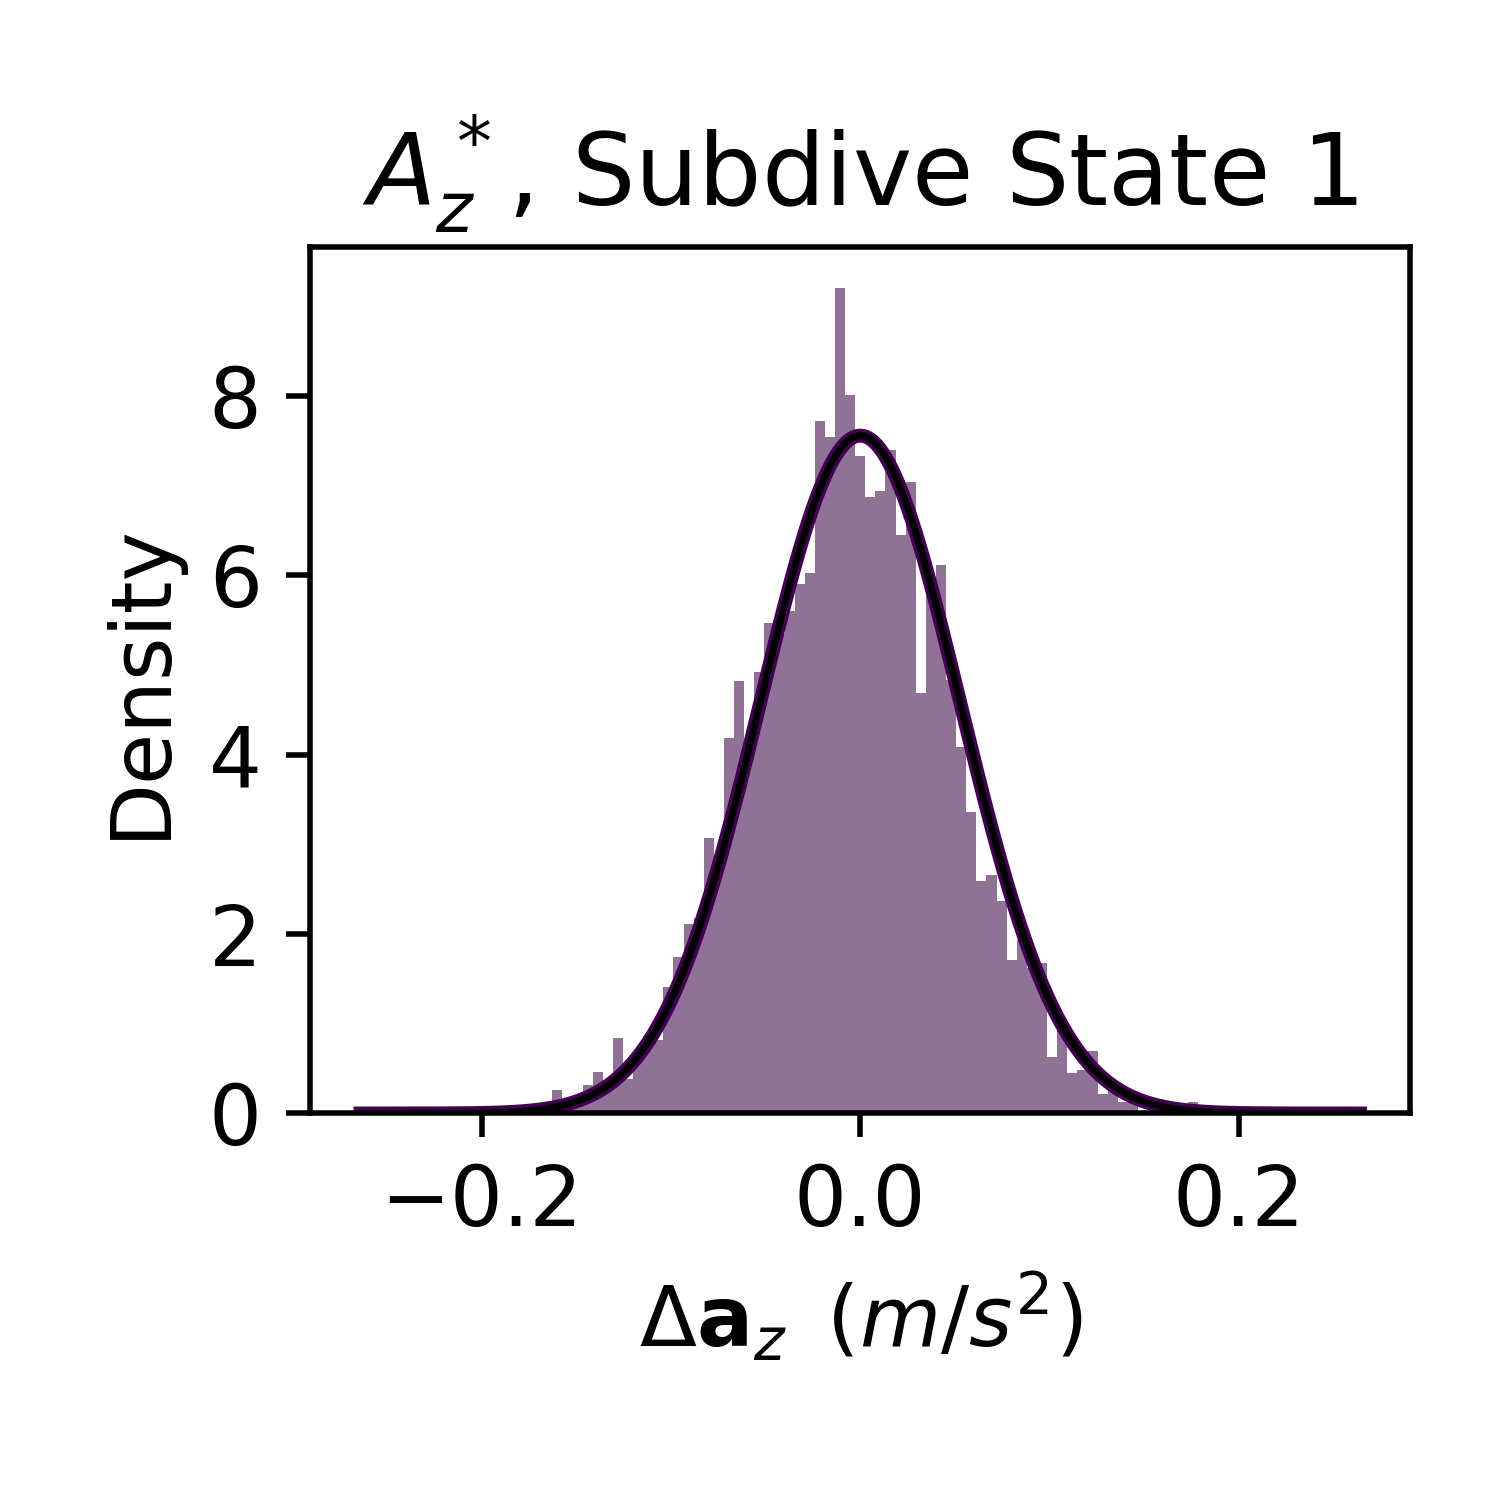
\includegraphics[width=1.75in]{../Plots/CarHHMM2_empirical_hist_Az_0.png}
        
        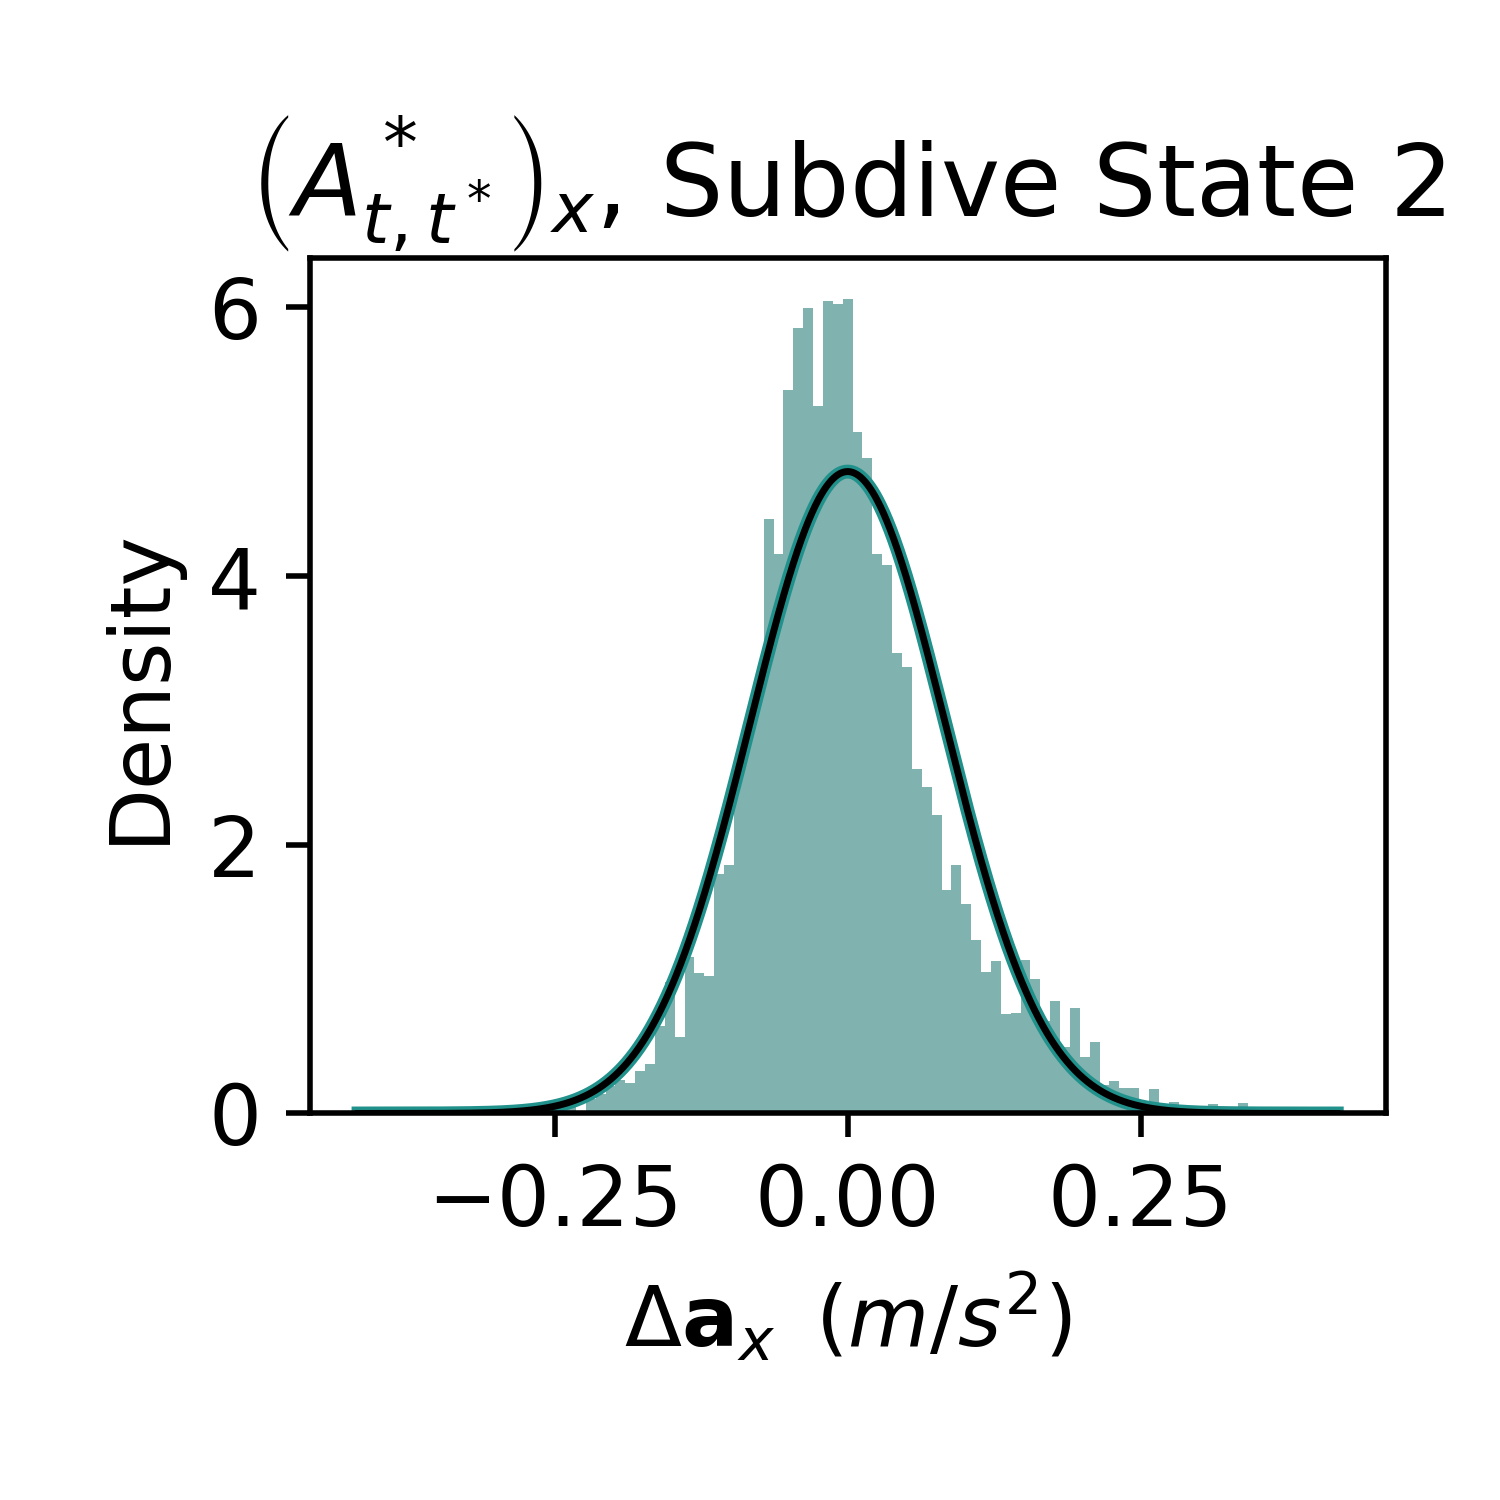
\includegraphics[width=1.75in]{../Plots/CarHHMM2_empirical_hist_Ax_1.png}
        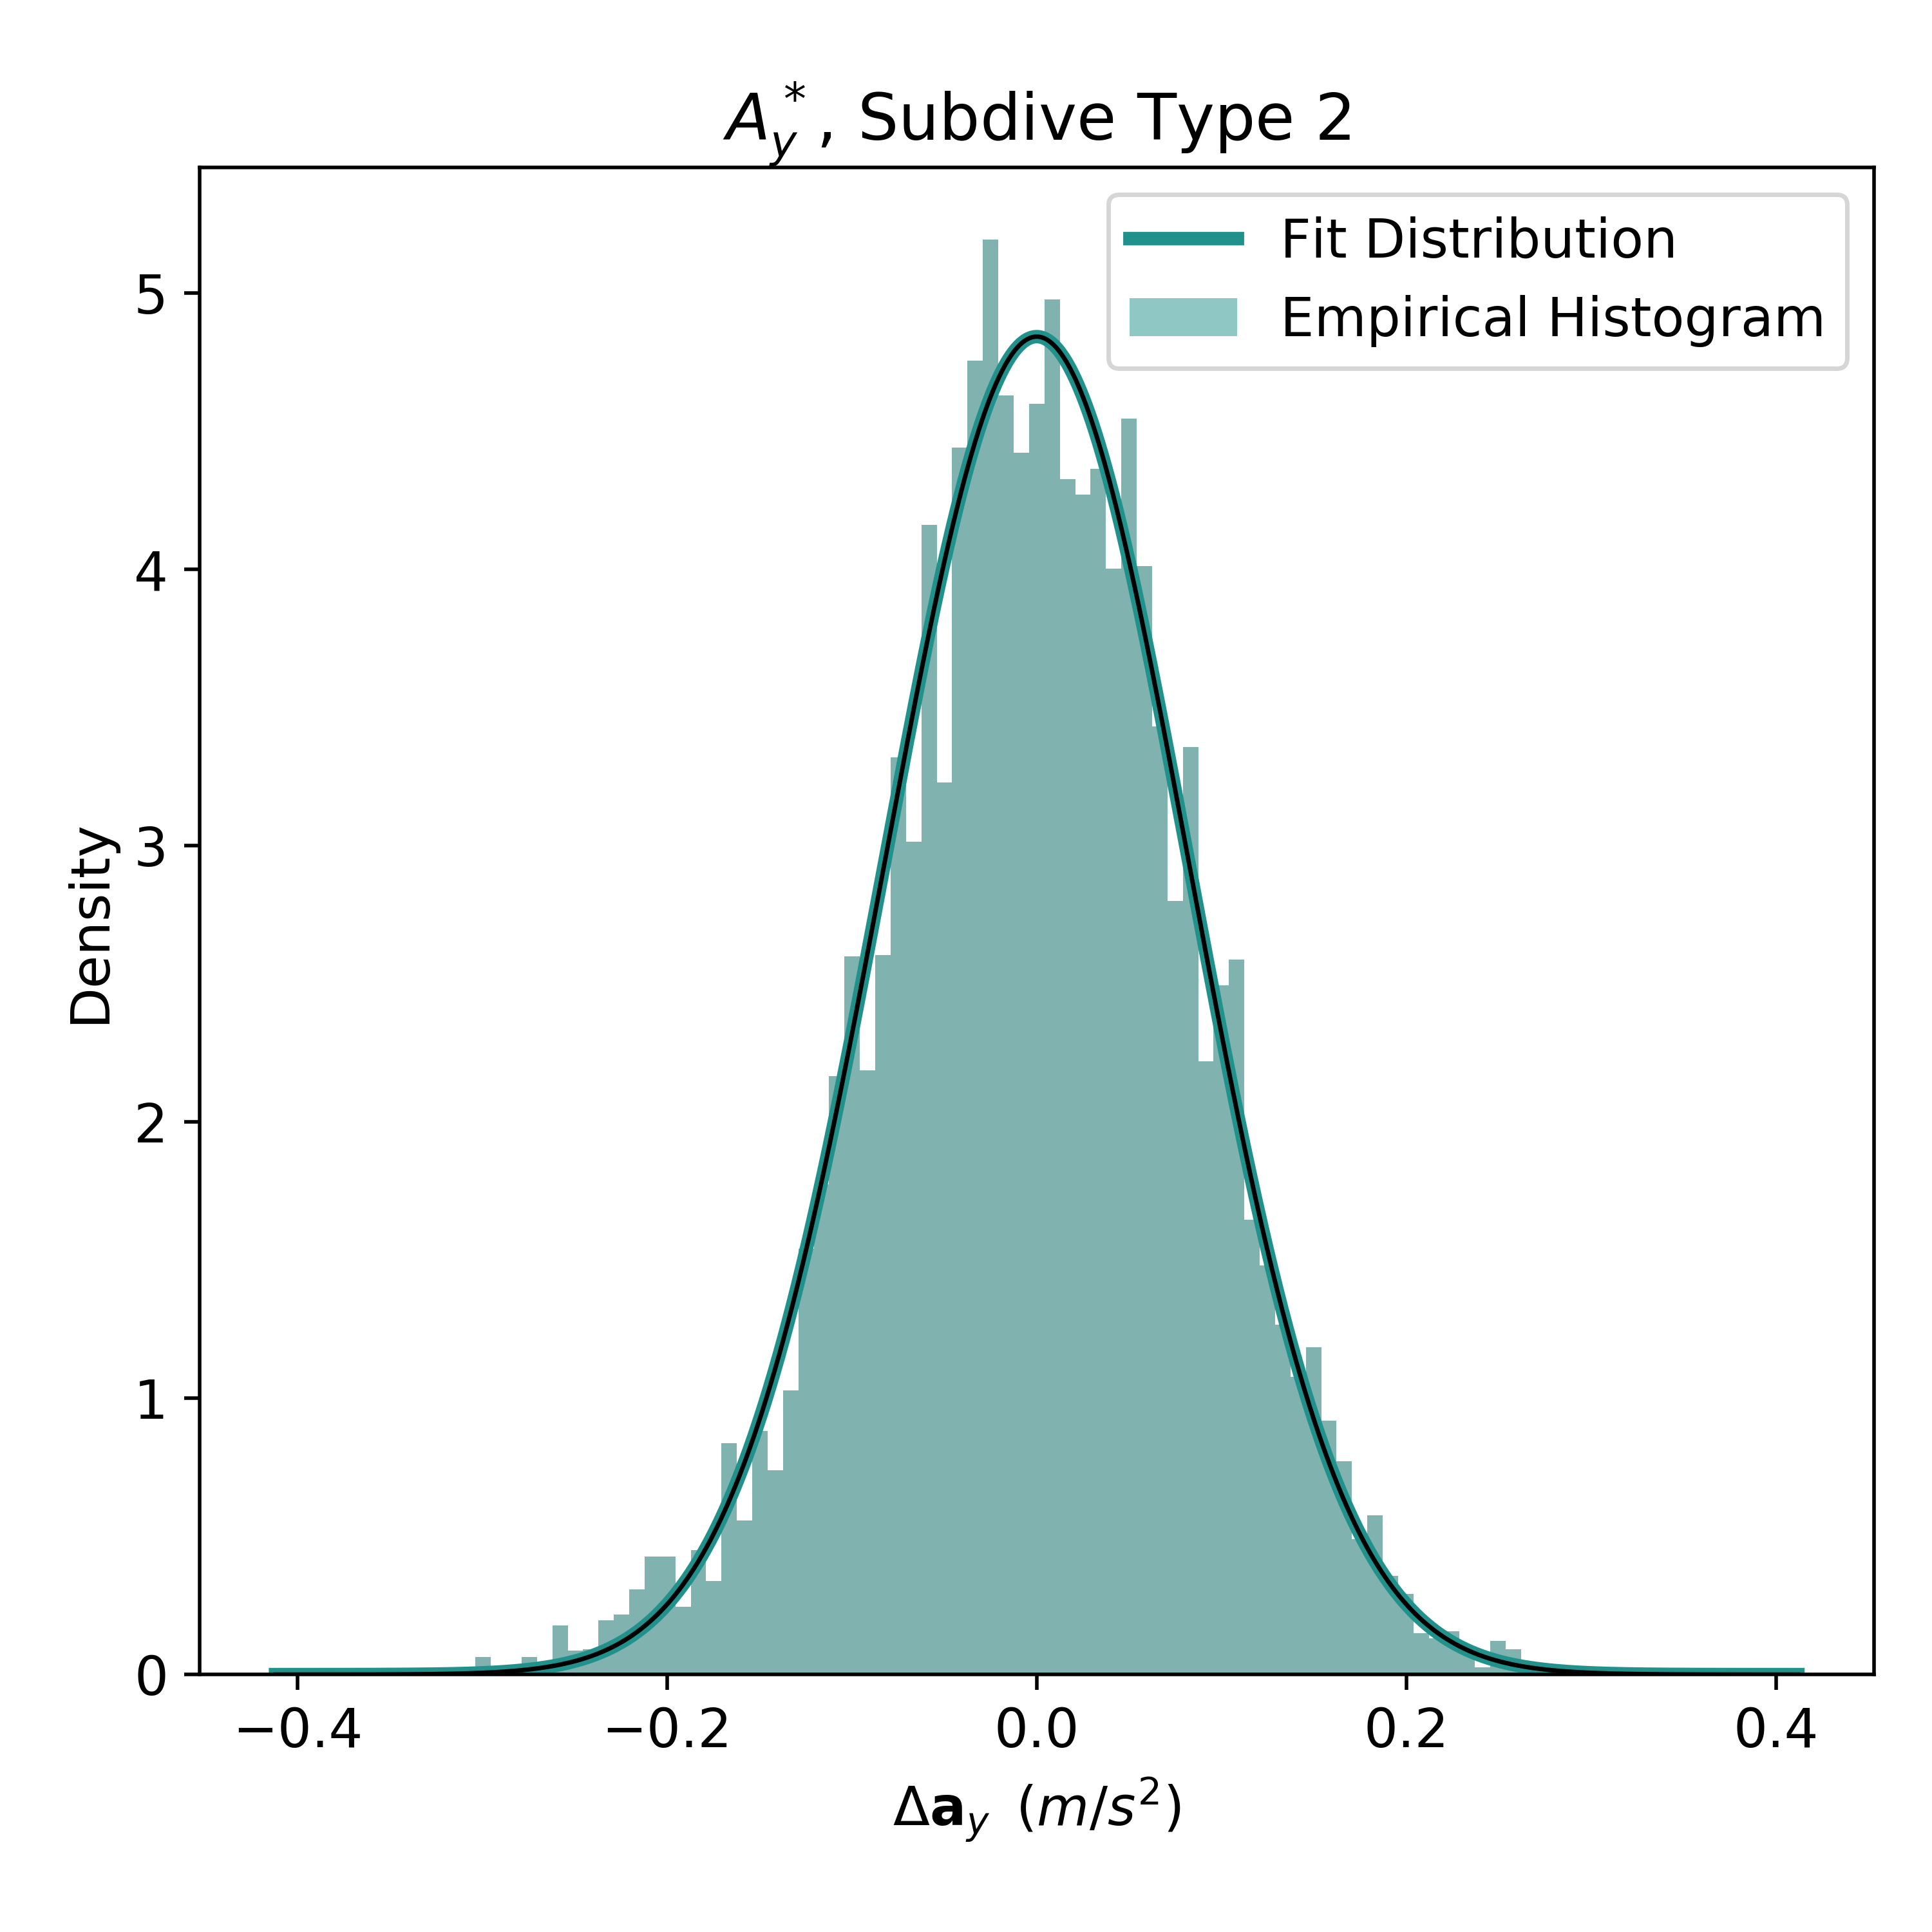
\includegraphics[width=1.75in]{../Plots/CarHHMM2_empirical_hist_Ay_1.png}
        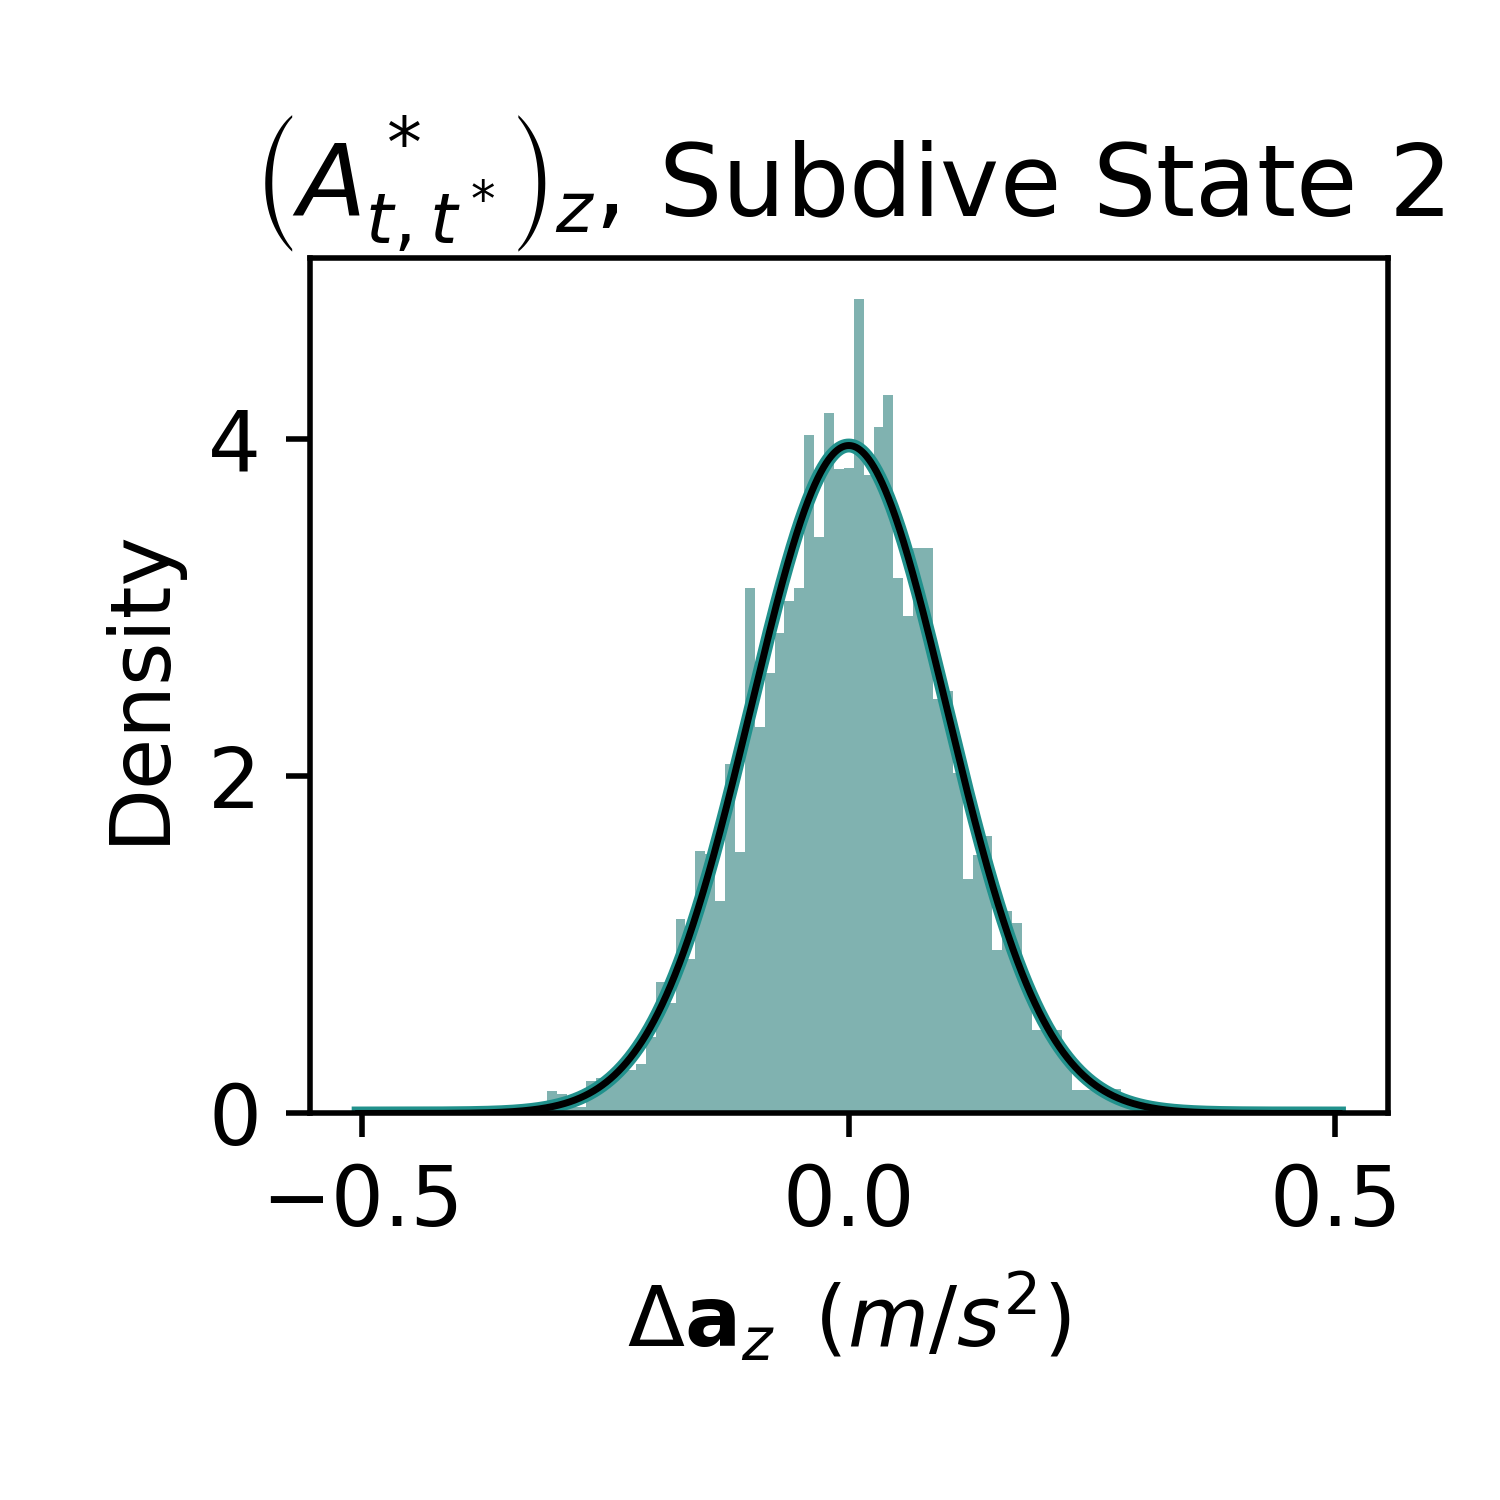
\includegraphics[width=1.75in]{../Plots/CarHHMM2_empirical_hist_Az_1.png}
        
        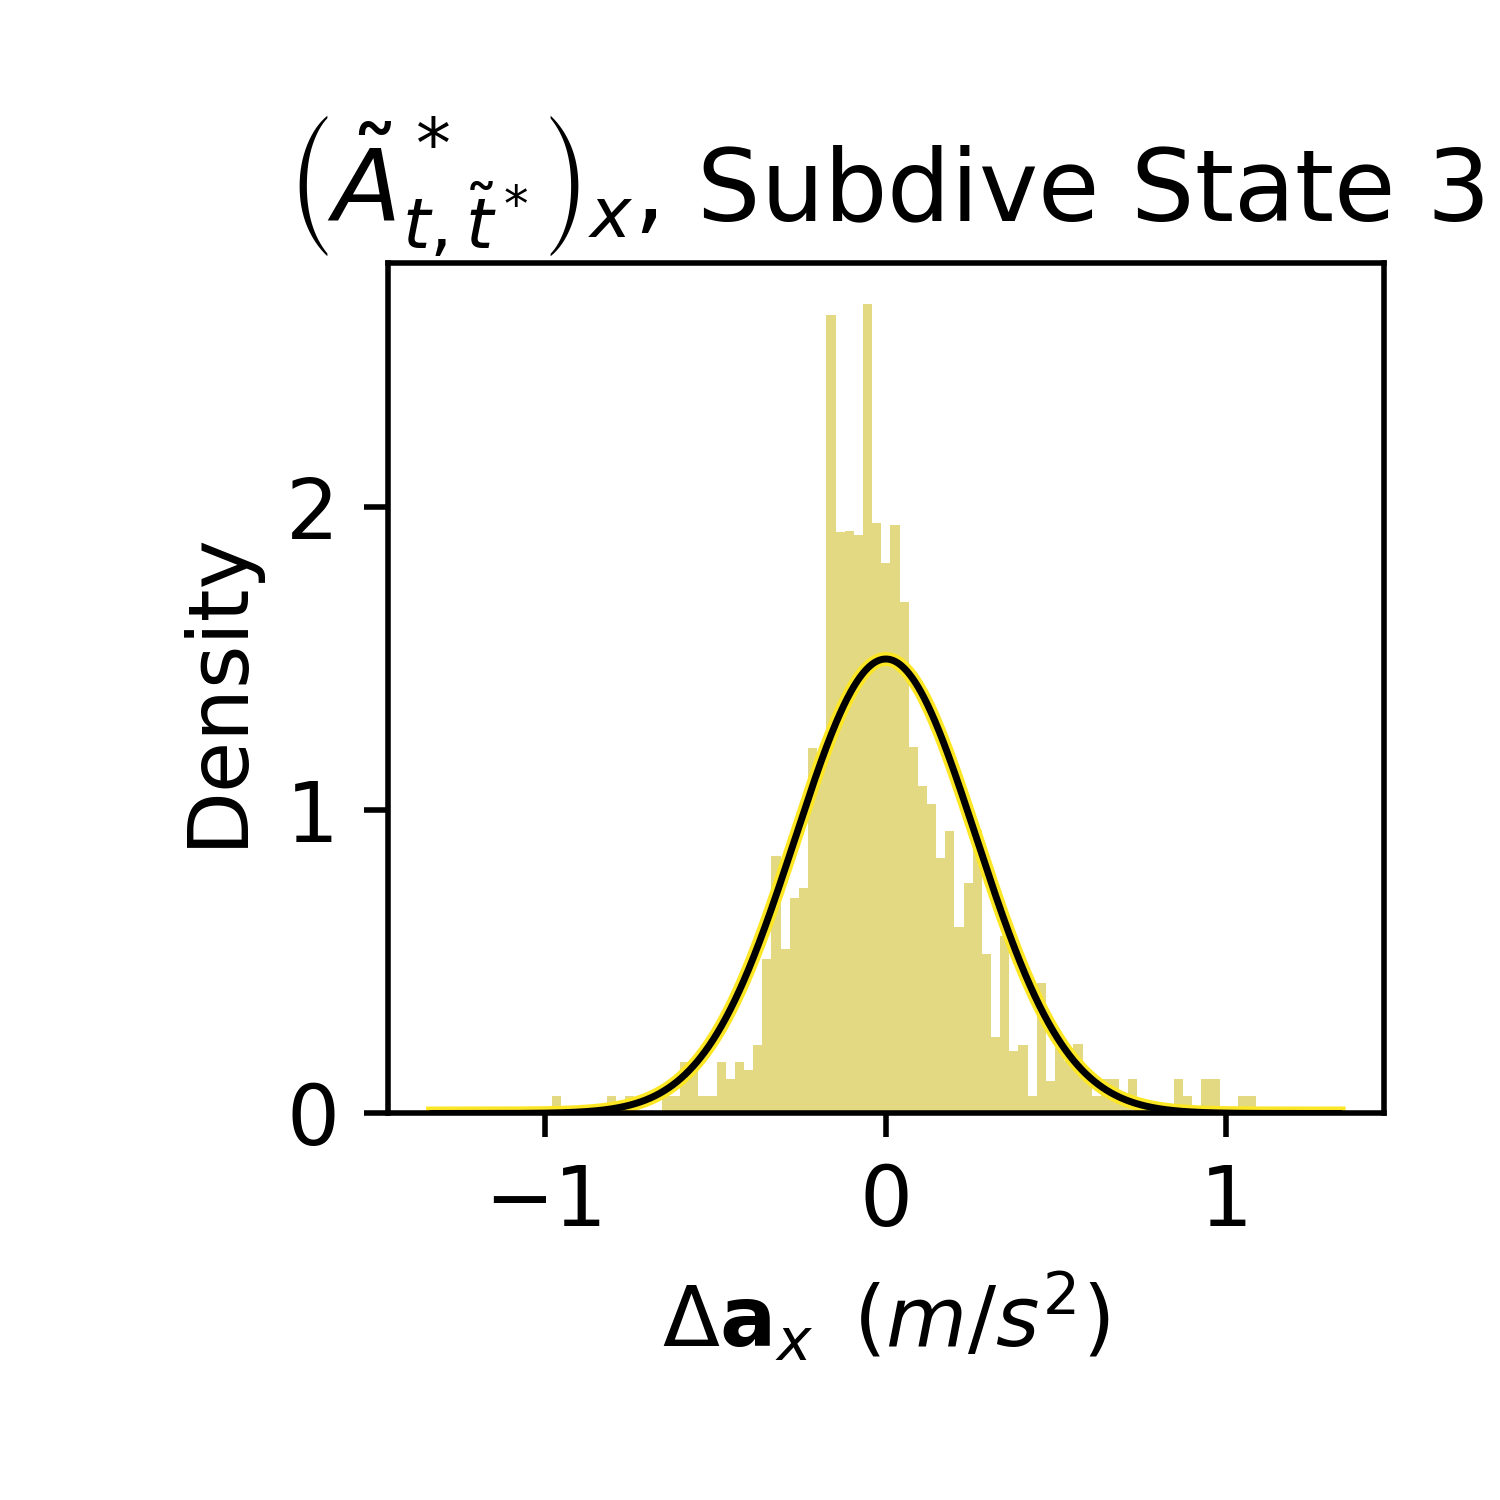
\includegraphics[width=1.75in]{../Plots/CarHHMM2_empirical_hist_Ax_2.png}
        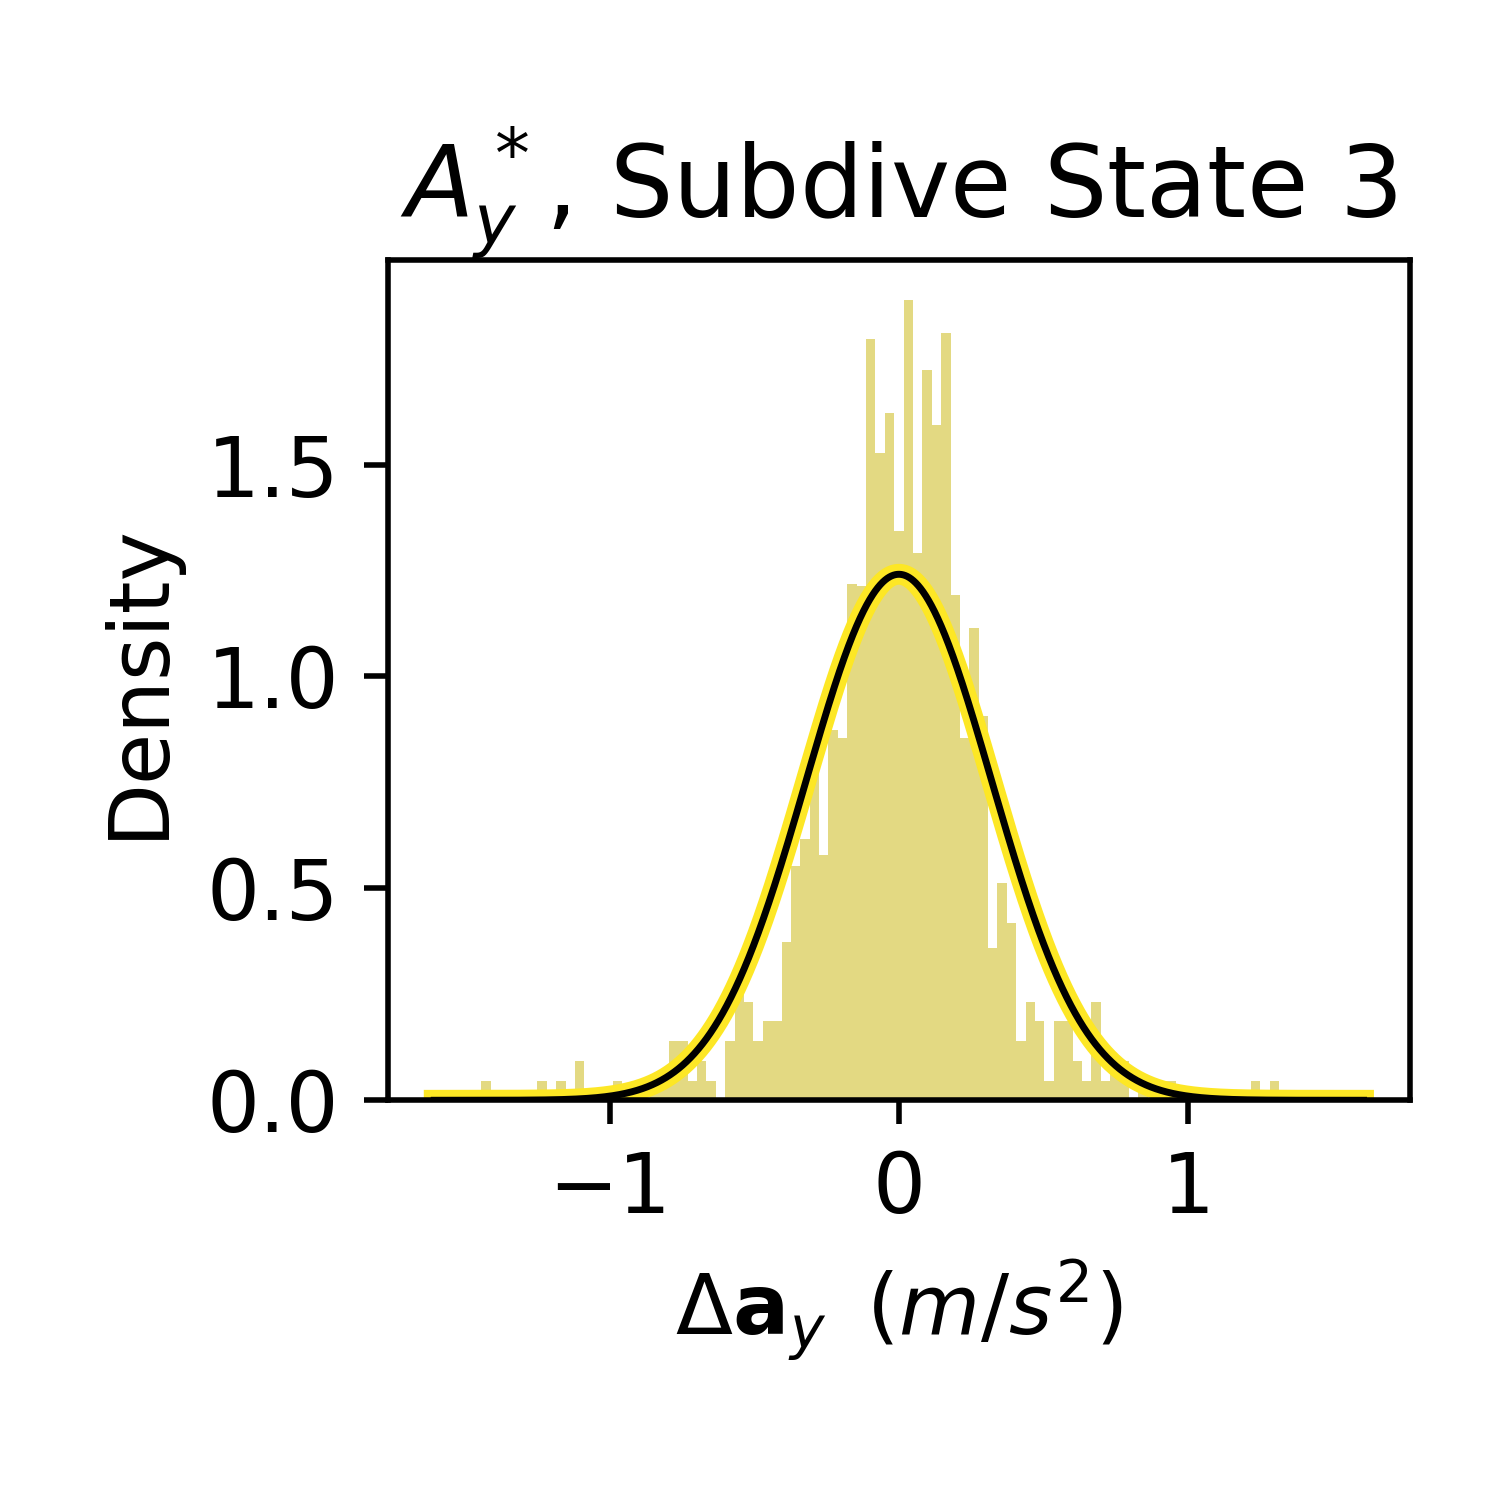
\includegraphics[width=1.75in]{../Plots/CarHHMM2_empirical_hist_Ay_2.png}
        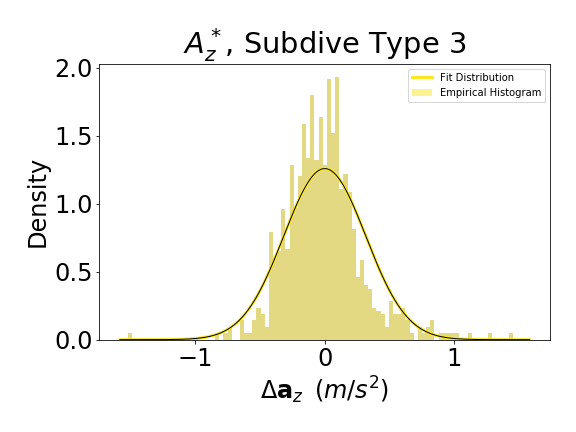
\includegraphics[width=1.75in]{../Plots/CarHHMM2_empirical_hist_Az_2.png}
        
        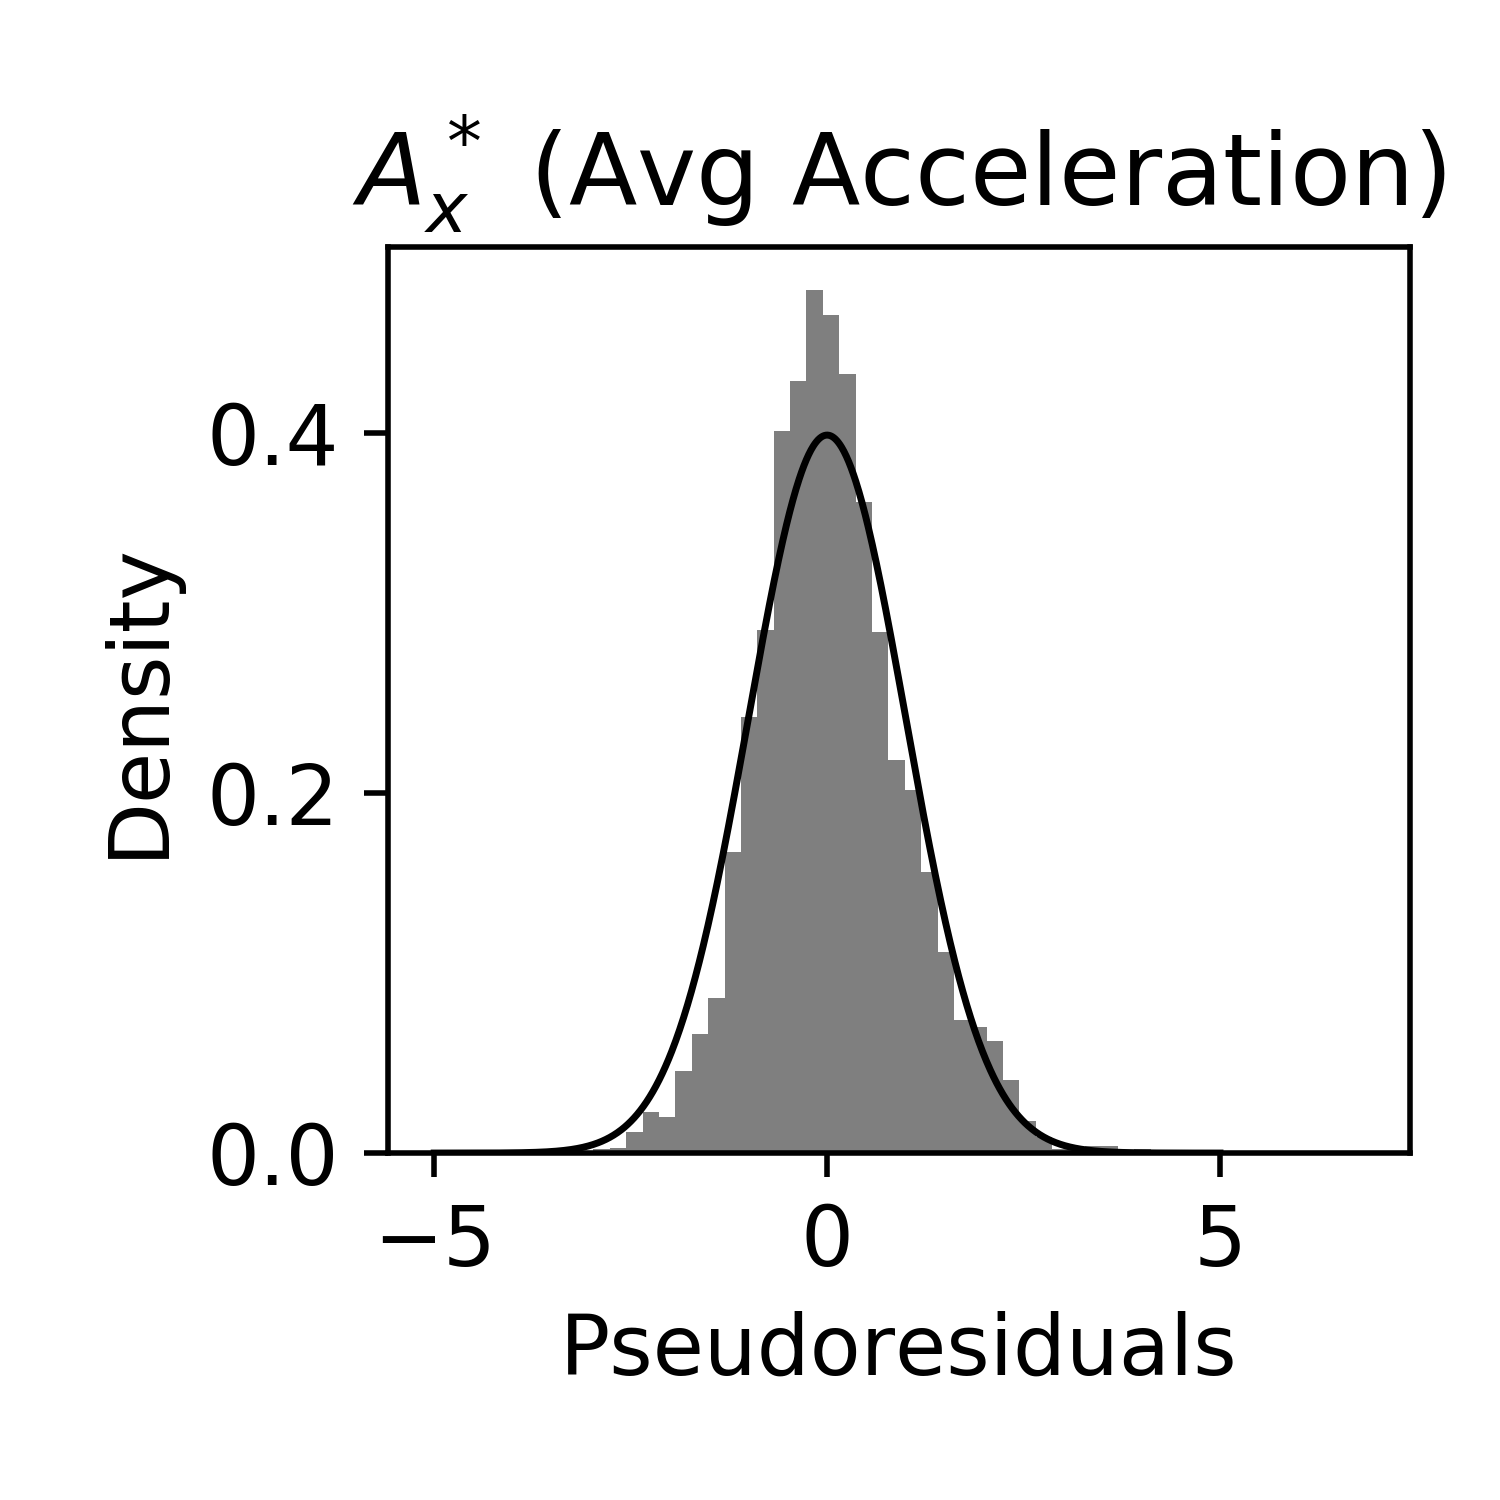
\includegraphics[width=1.75in]{../Plots/CarHHMM2_psedoresids_Ax.png}
        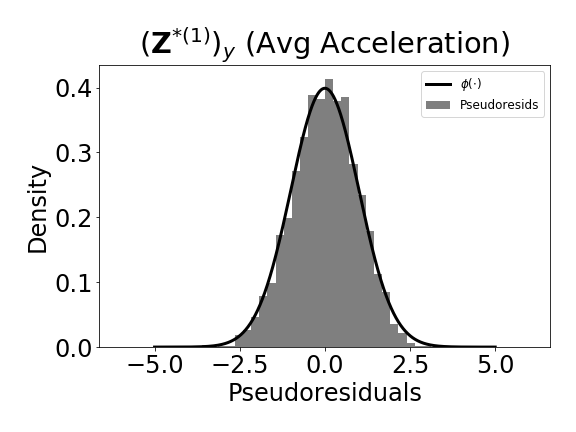
\includegraphics[width=1.75in]{../Plots/CarHHMM2_psedoresids_Ay.png}
        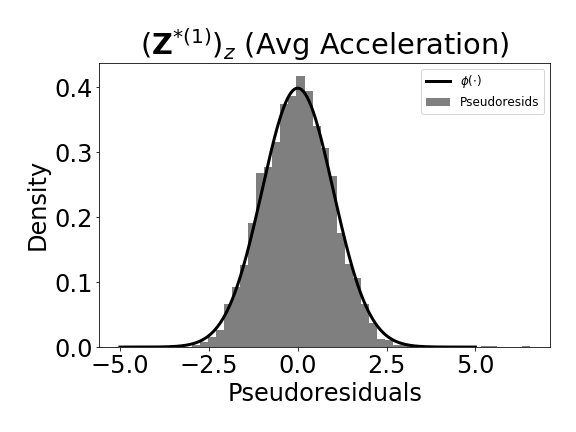
\includegraphics[width=1.75in]{../Plots/CarHHMM2_psedoresids_Az.png}
        \end{center}
        
        \noindent Figure \arabic{fignum}: Empirical histograms (top three rows) and psuedoresiduals (bottom row) of acceleration ($\Zone_{t,t^*}$) plotted over the learned emission distributions and a standard normal density, respectively. Note that the mean of acceleration at time $t^*$ depends upon acceleration at time $t^*-1$, so only the deviation from the mean for each particular time step is plotted. All plots are generated using the fitted CarHHMM-DFT and the killer whale case study data.
        \addtocounter{fignum}{1}
        
        \newpage
        
        \subsubsection{HHMM-DFT}
        
        \begin{center}
        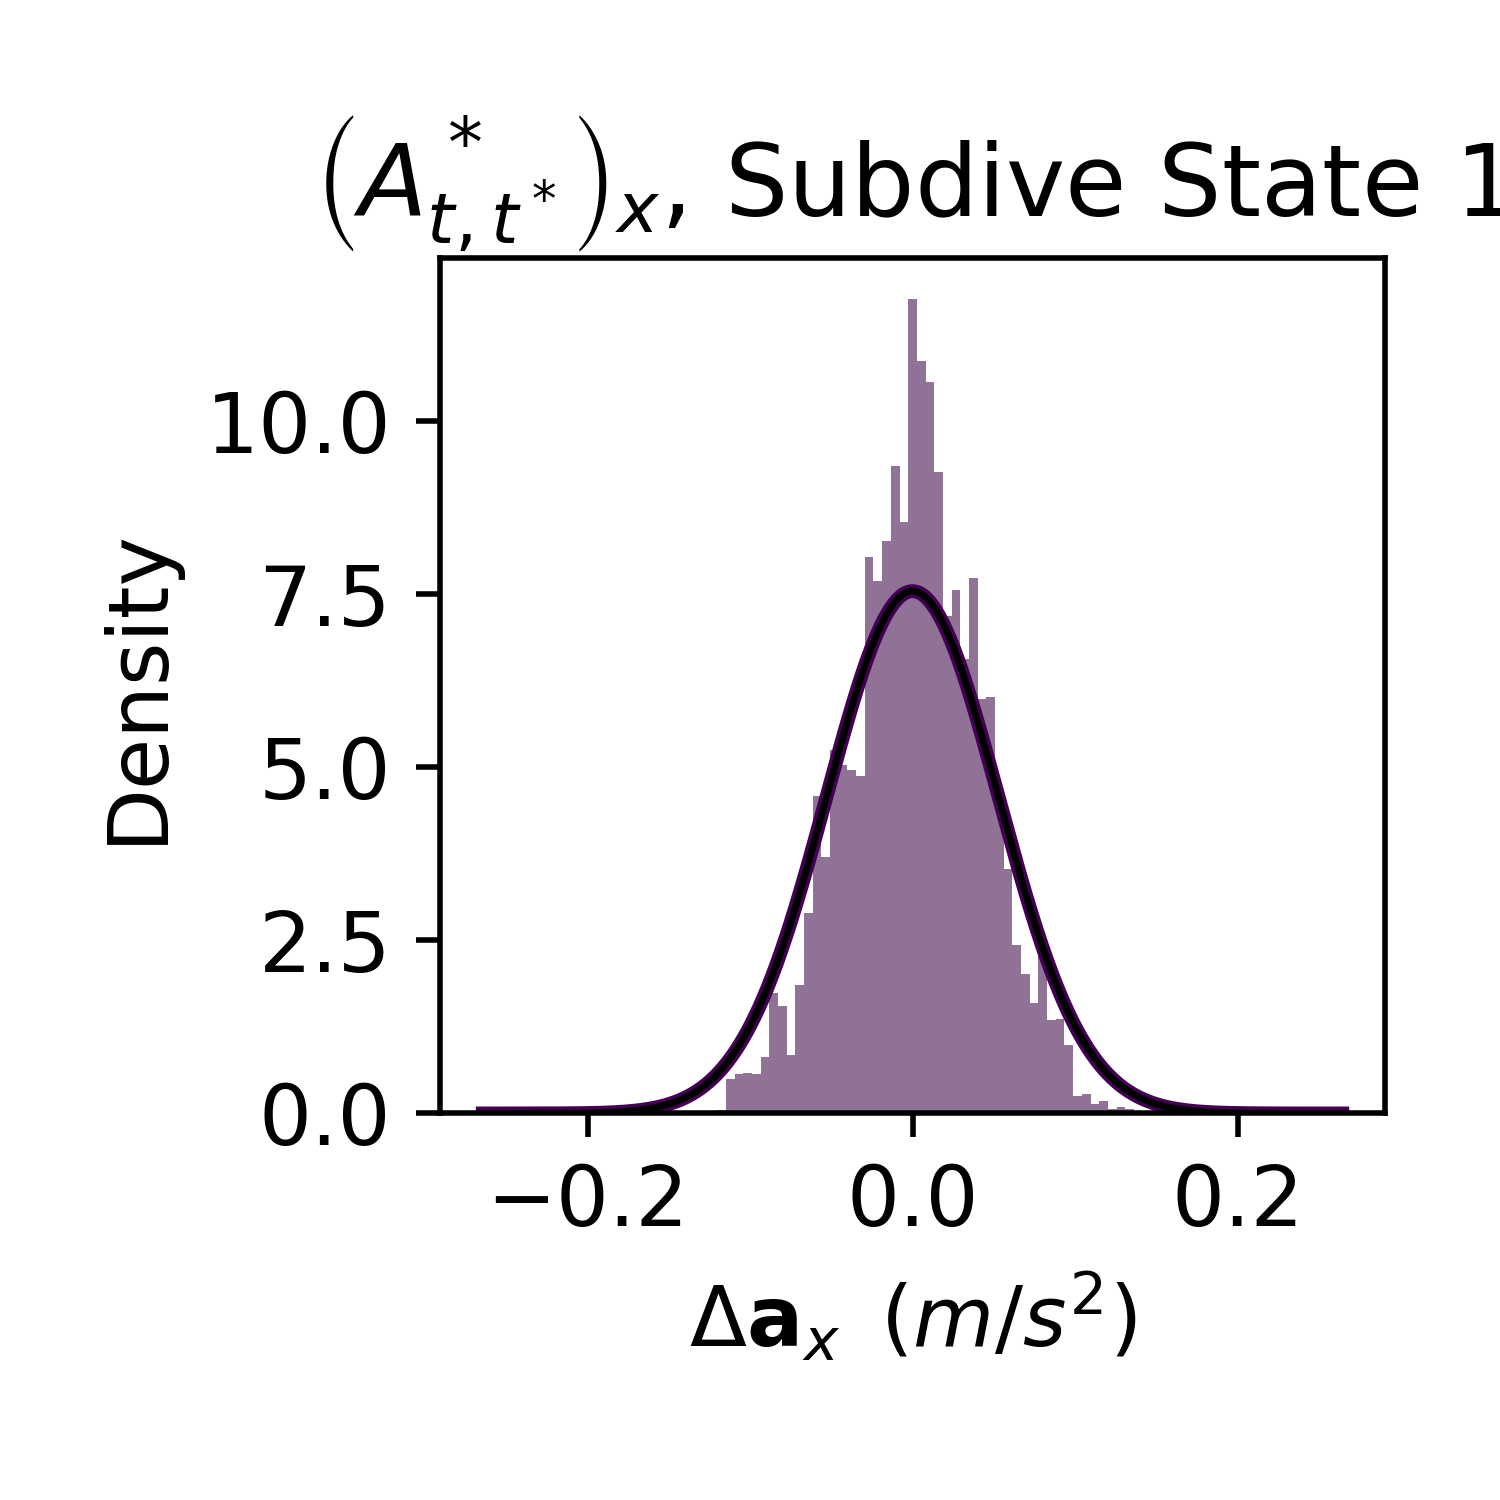
\includegraphics[width=1.75in]{../Plots/HHMM_empirical_hist_Ax_0.png}
        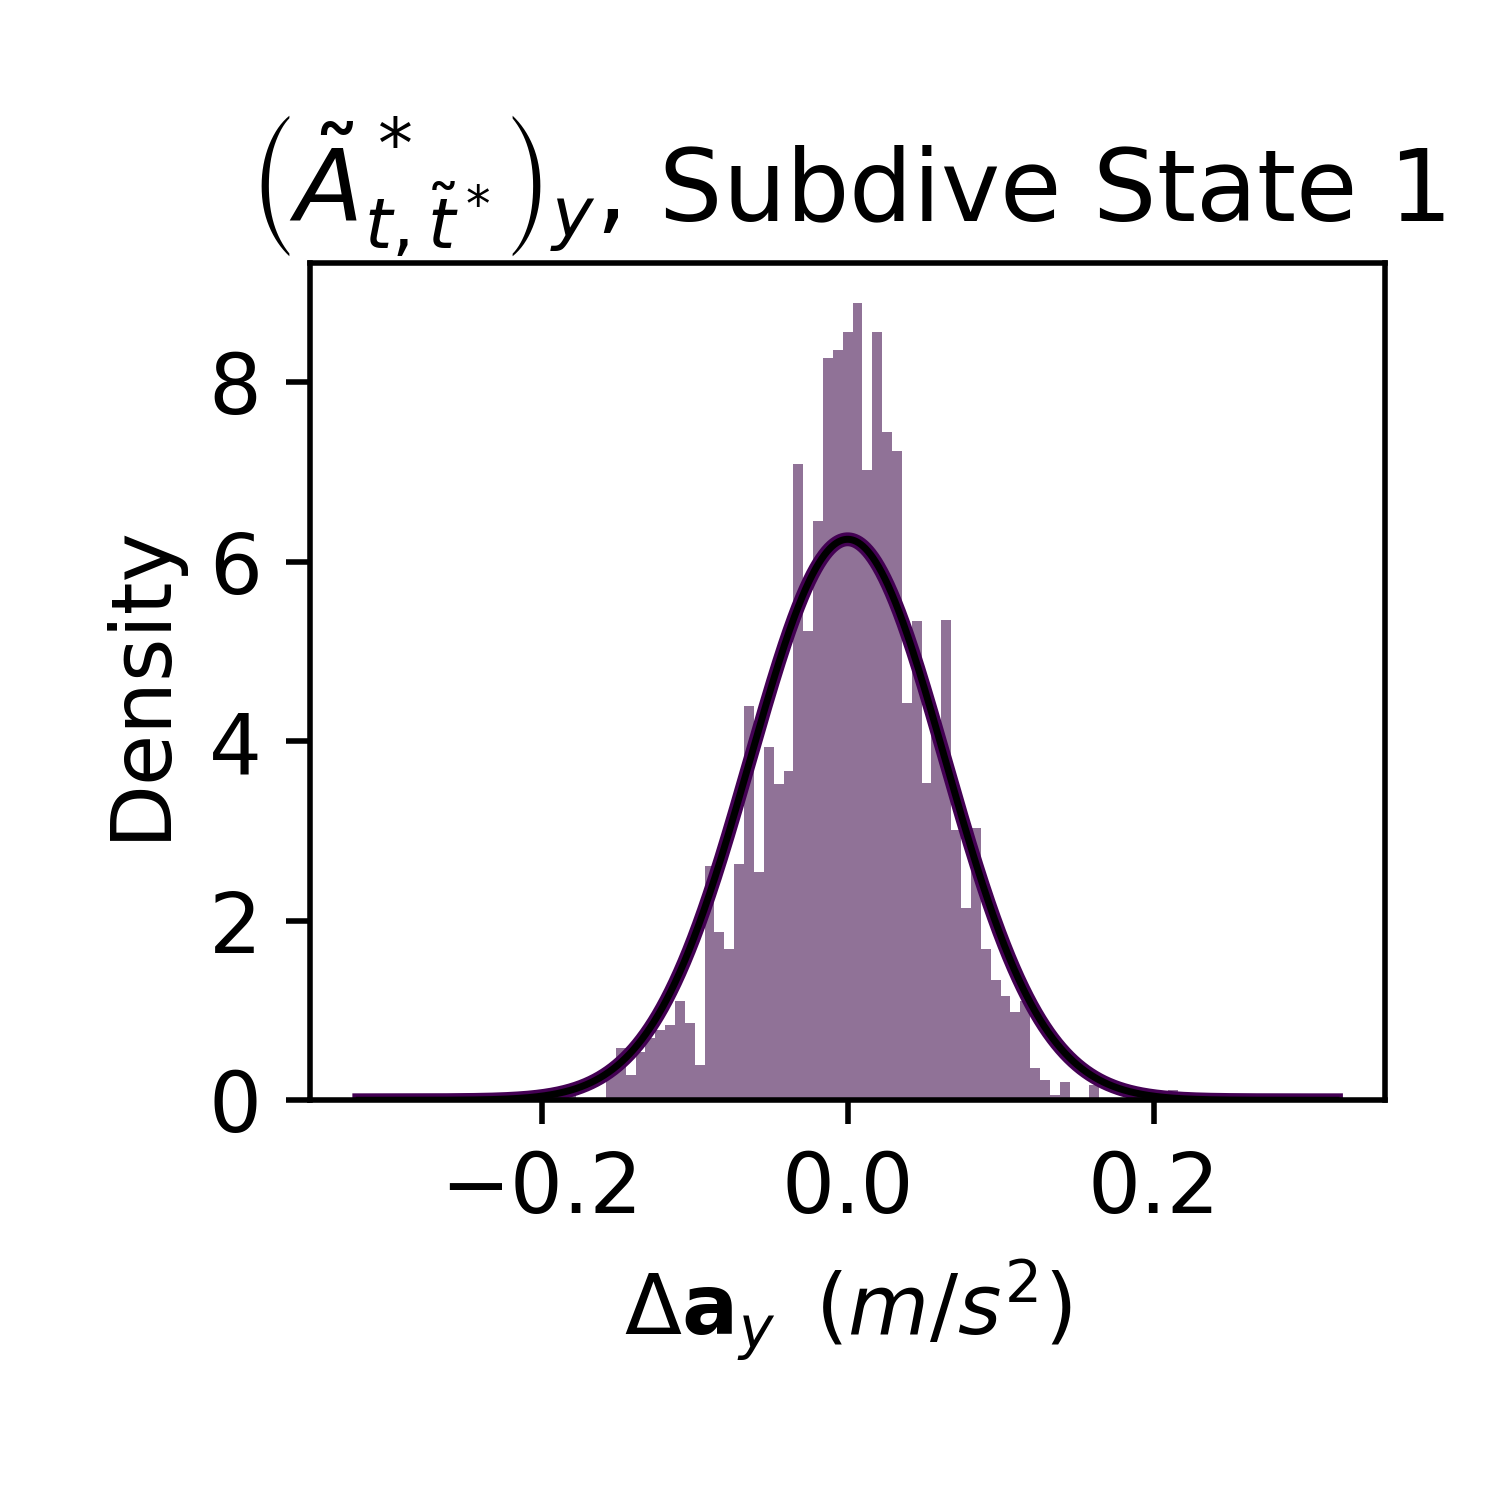
\includegraphics[width=1.75in]{../Plots/HHMM_empirical_hist_Ay_0.png}
        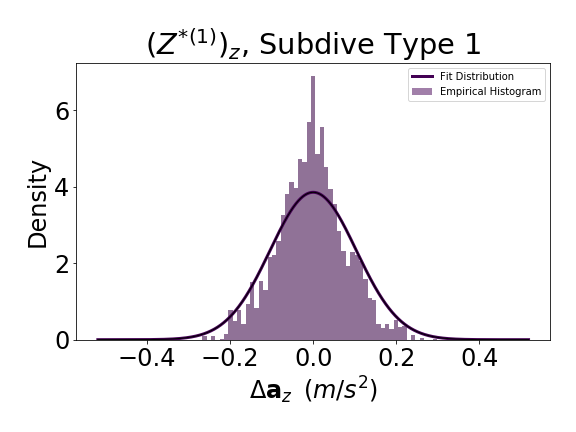
\includegraphics[width=1.75in]{../Plots/HHMM_empirical_hist_Az_0.png}
        
        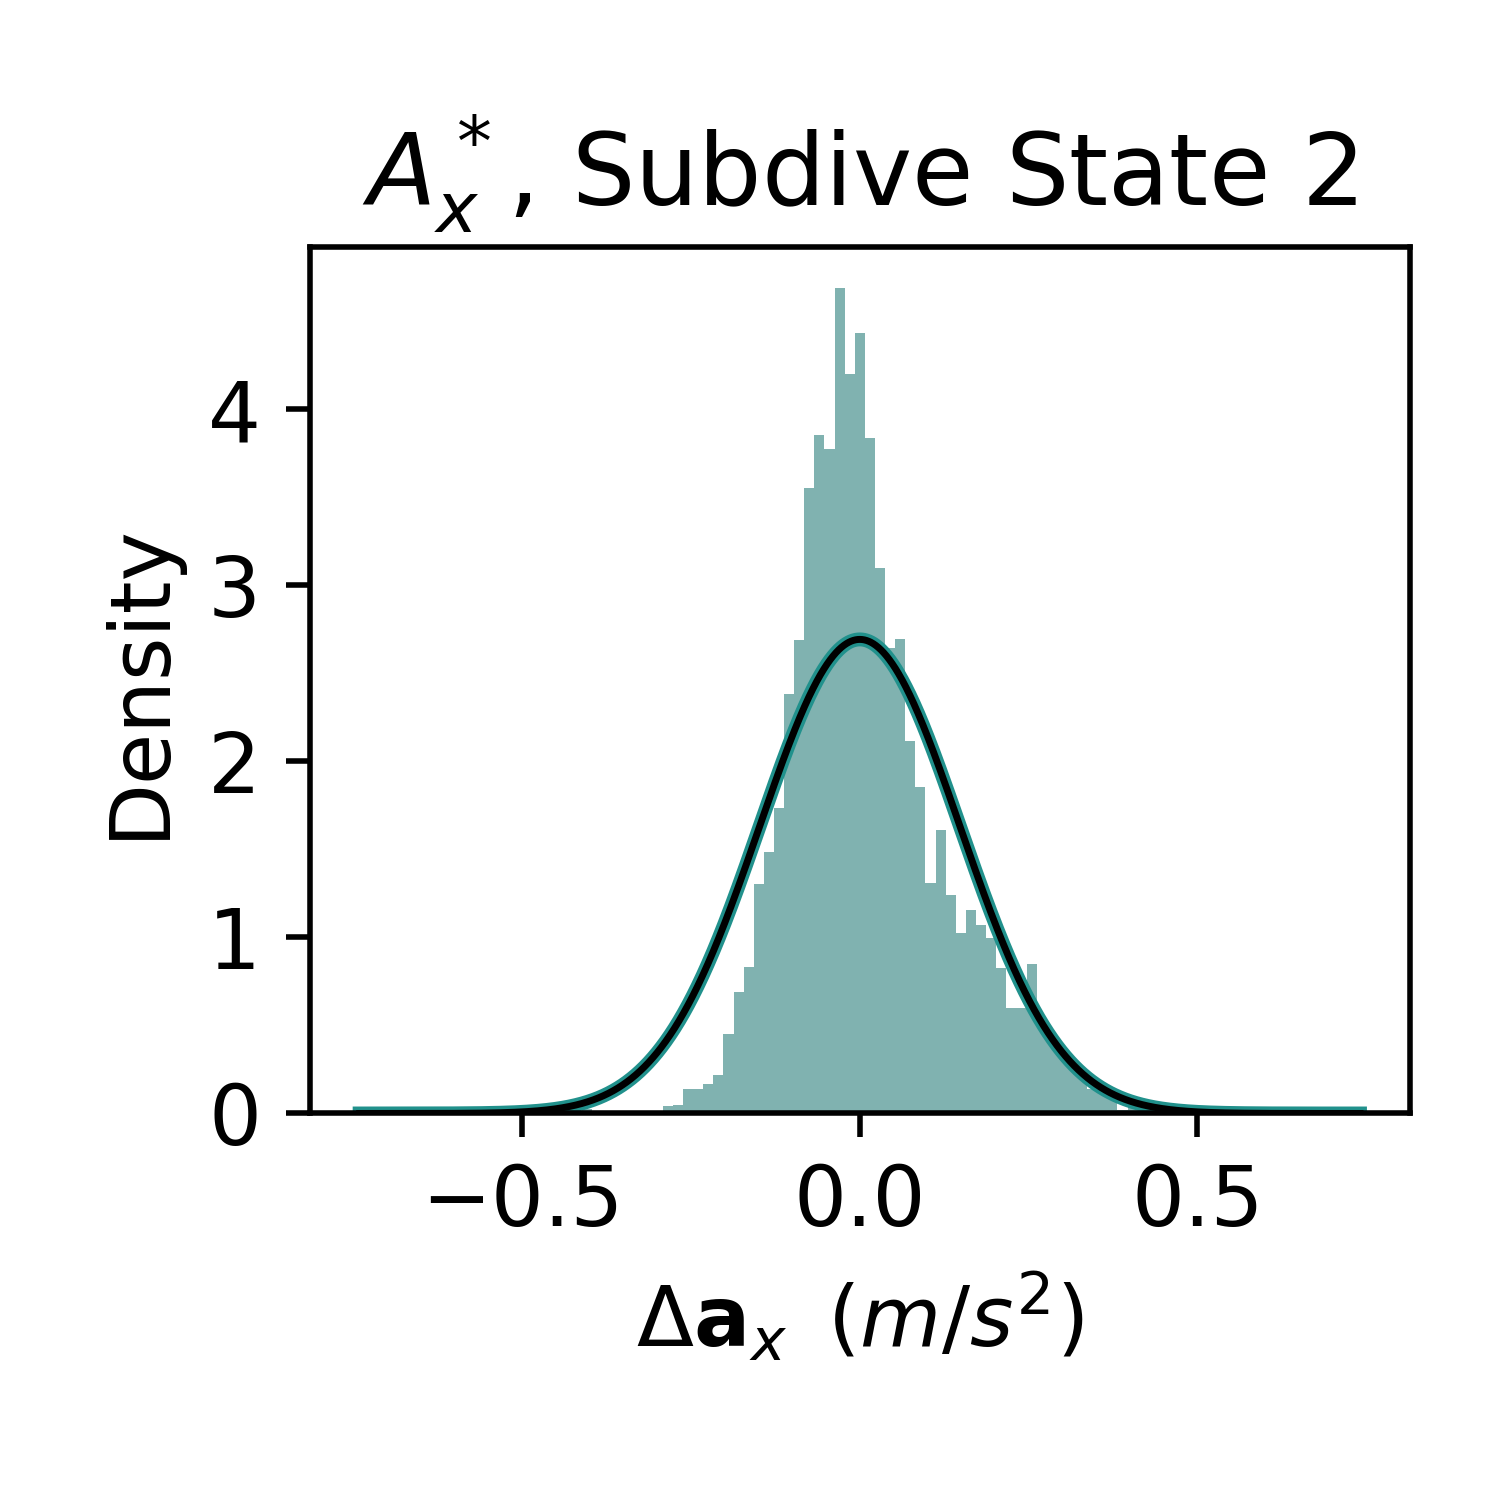
\includegraphics[width=1.75in]{../Plots/HHMM_empirical_hist_Ax_1.png}
        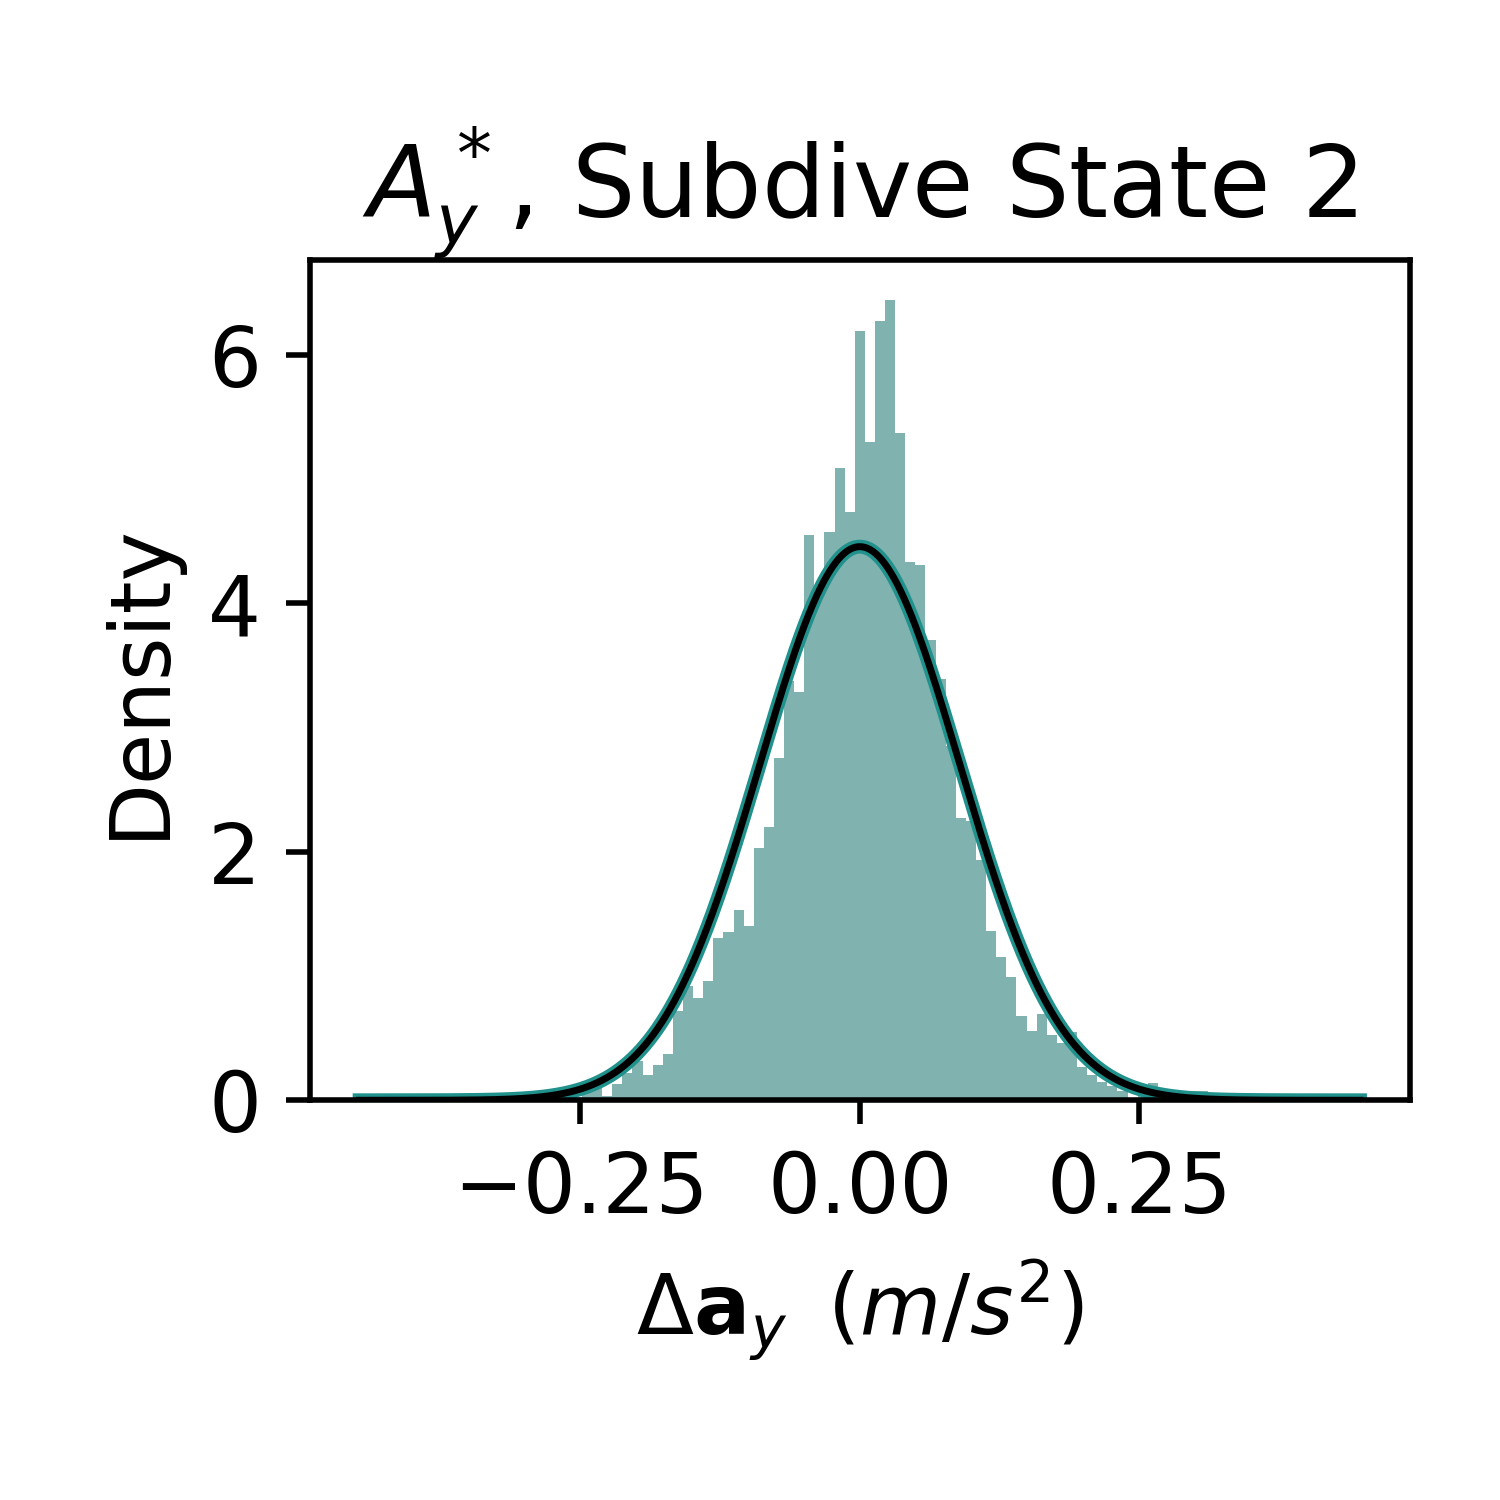
\includegraphics[width=1.75in]{../Plots/HHMM_empirical_hist_Ay_1.png}
        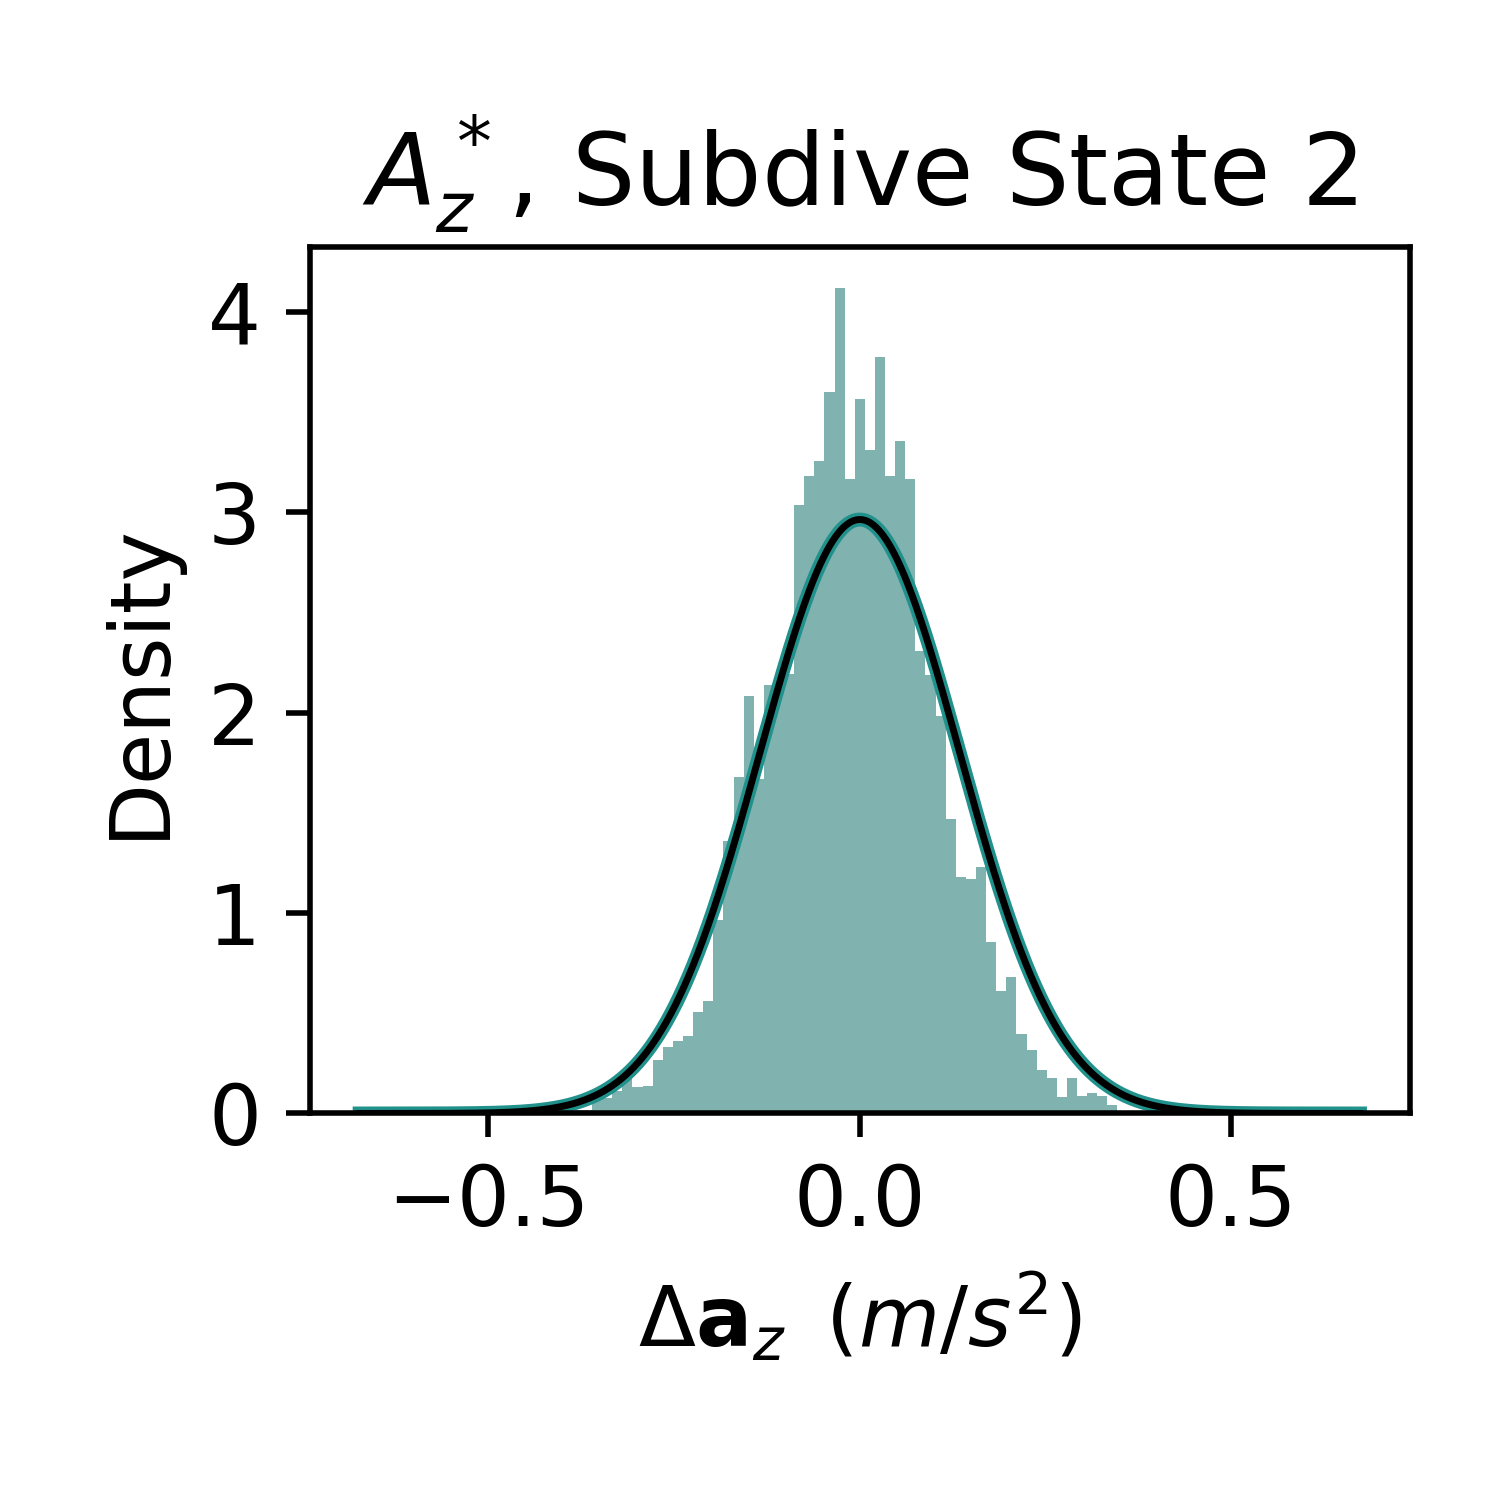
\includegraphics[width=1.75in]{../Plots/HHMM_empirical_hist_Az_1.png}
        
        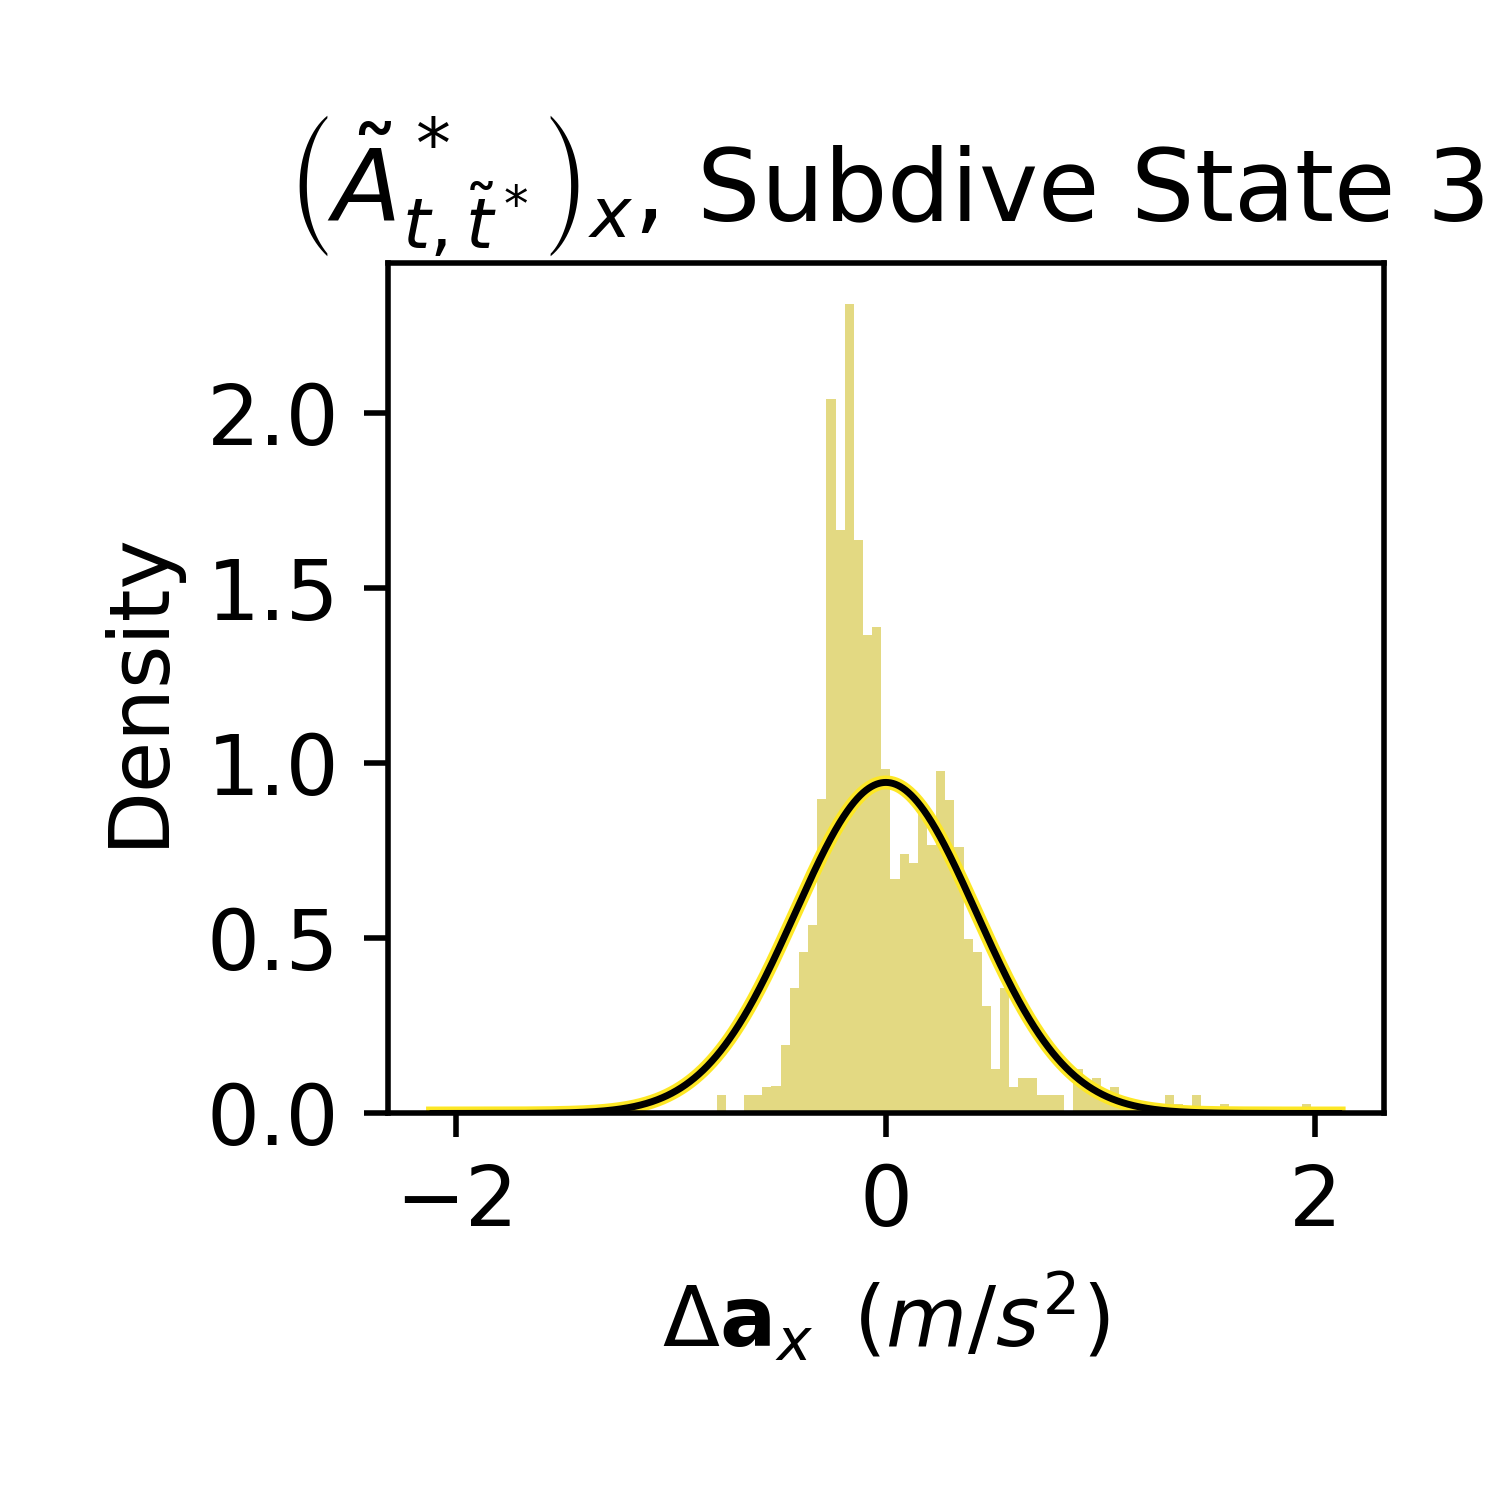
\includegraphics[width=1.75in]{../Plots/HHMM_empirical_hist_Ax_2.png}
        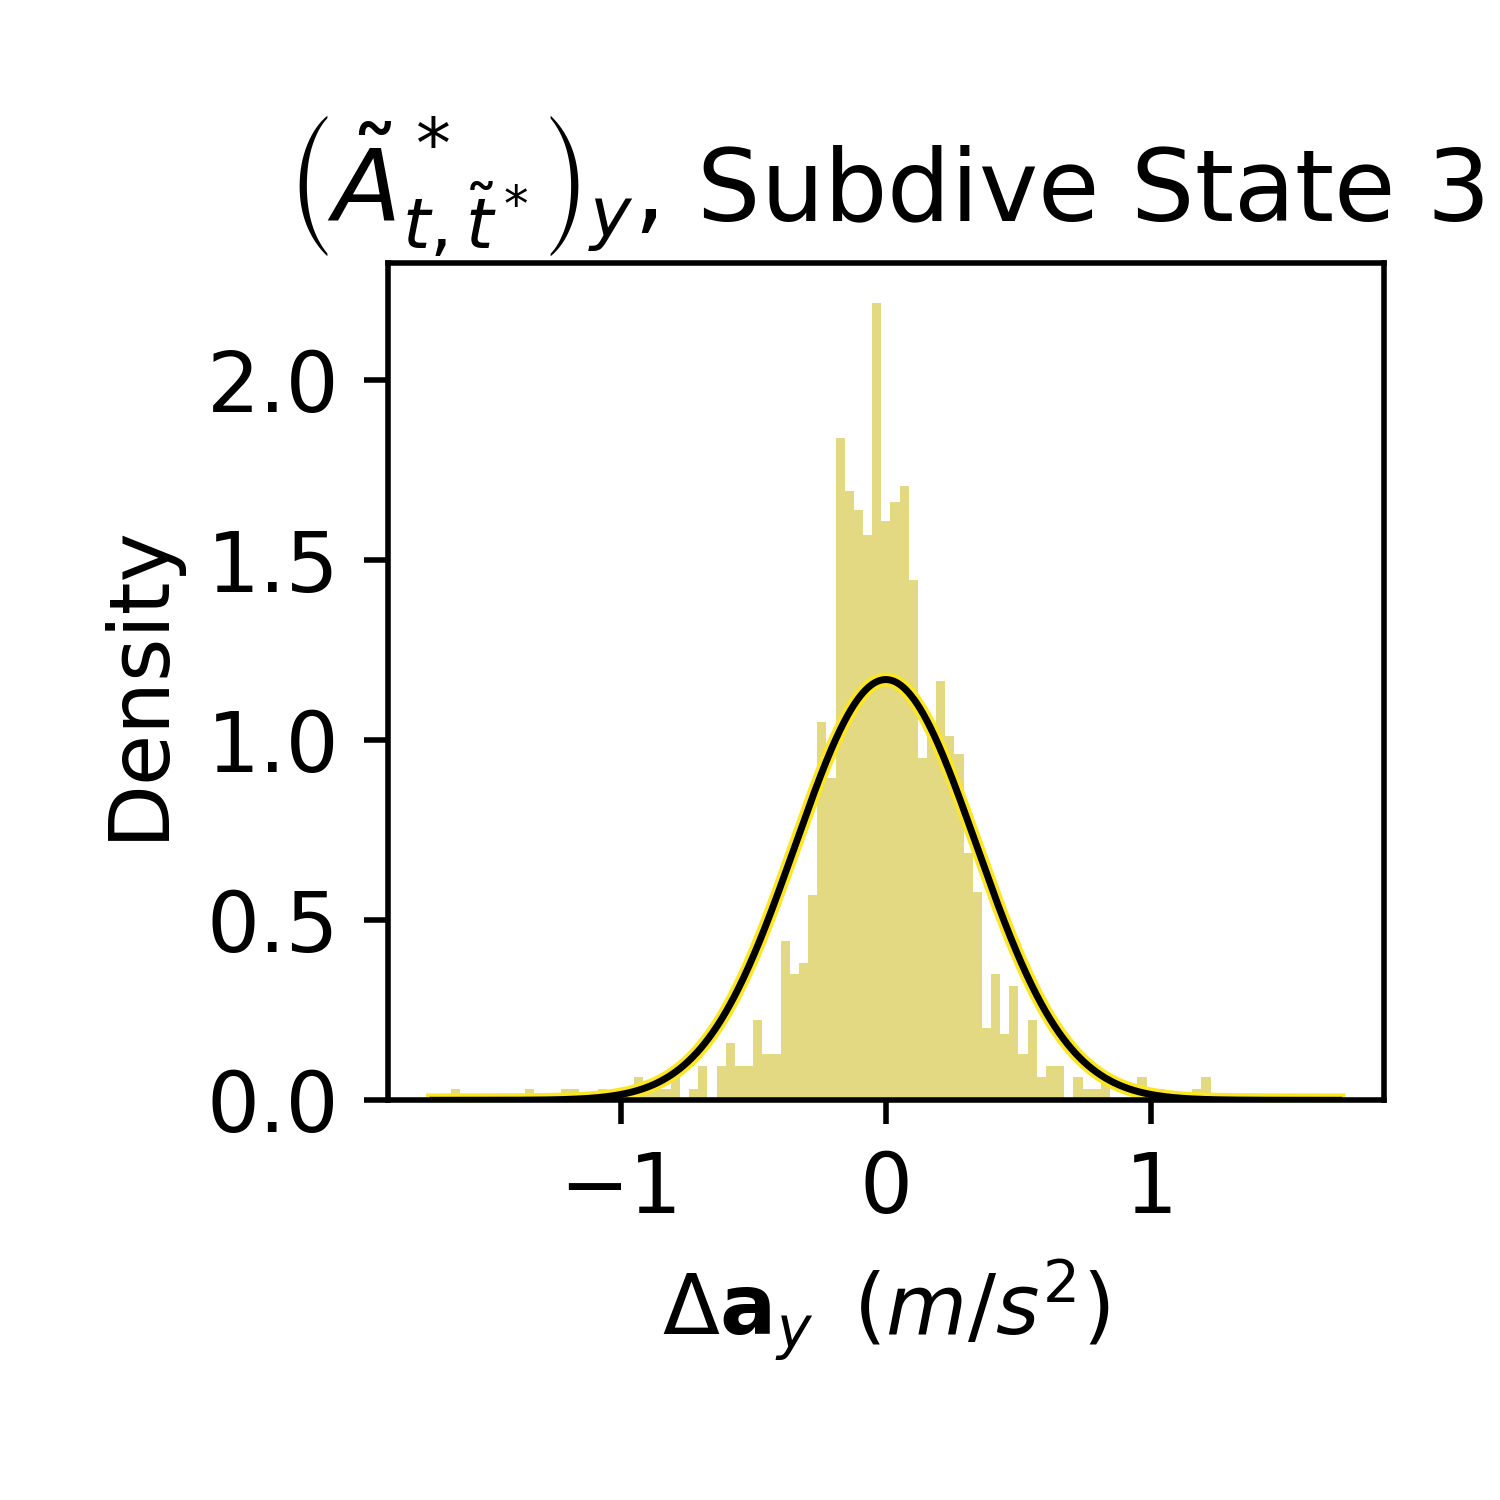
\includegraphics[width=1.75in]{../Plots/HHMM_empirical_hist_Ay_2.png}
        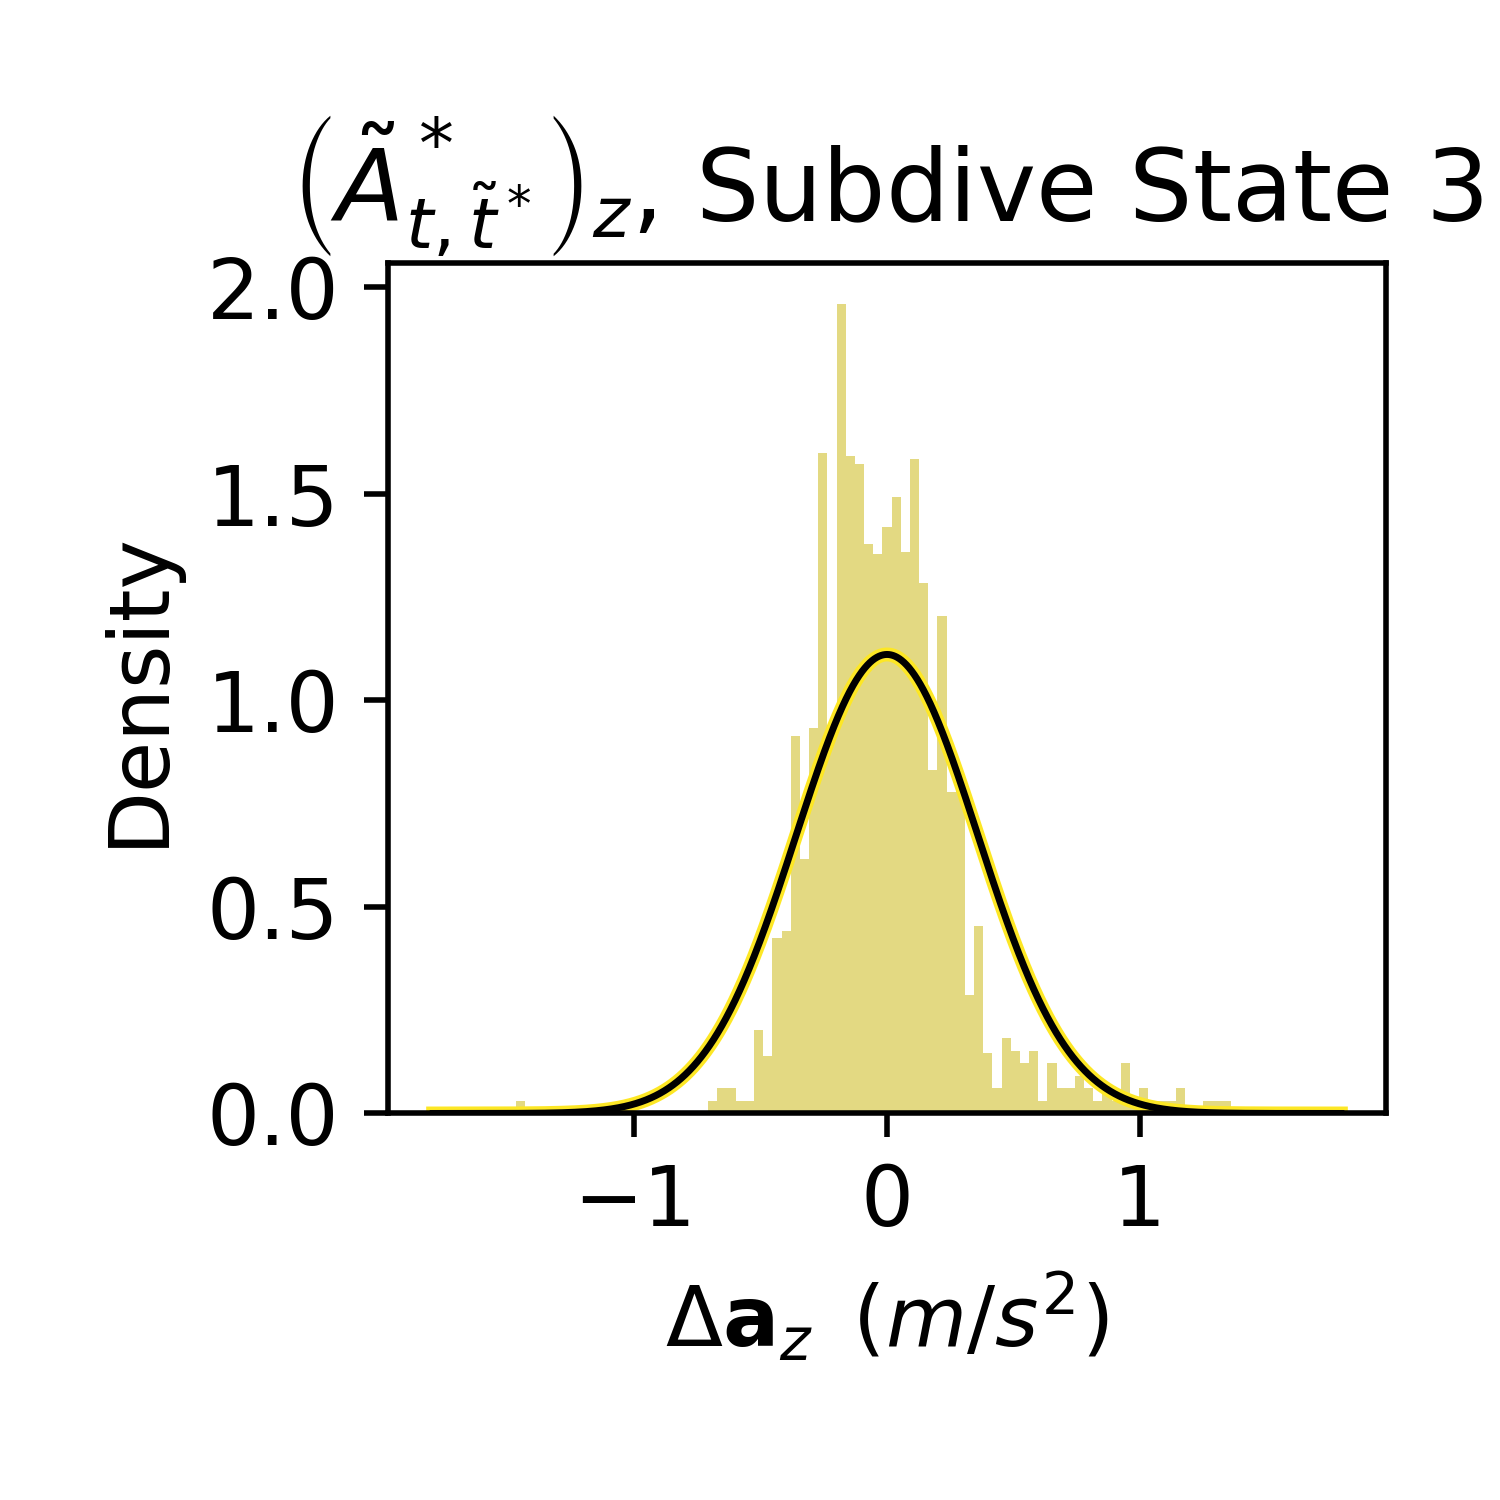
\includegraphics[width=1.75in]{../Plots/HHMM_empirical_hist_Az_2.png}
        
        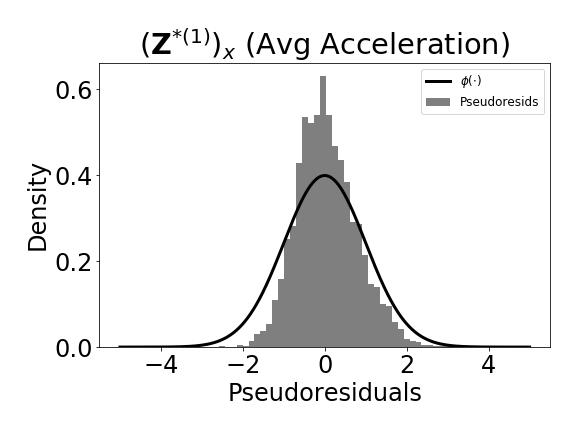
\includegraphics[width=1.75in]{../Plots/HHMM_psedoresids_Ax.png}
        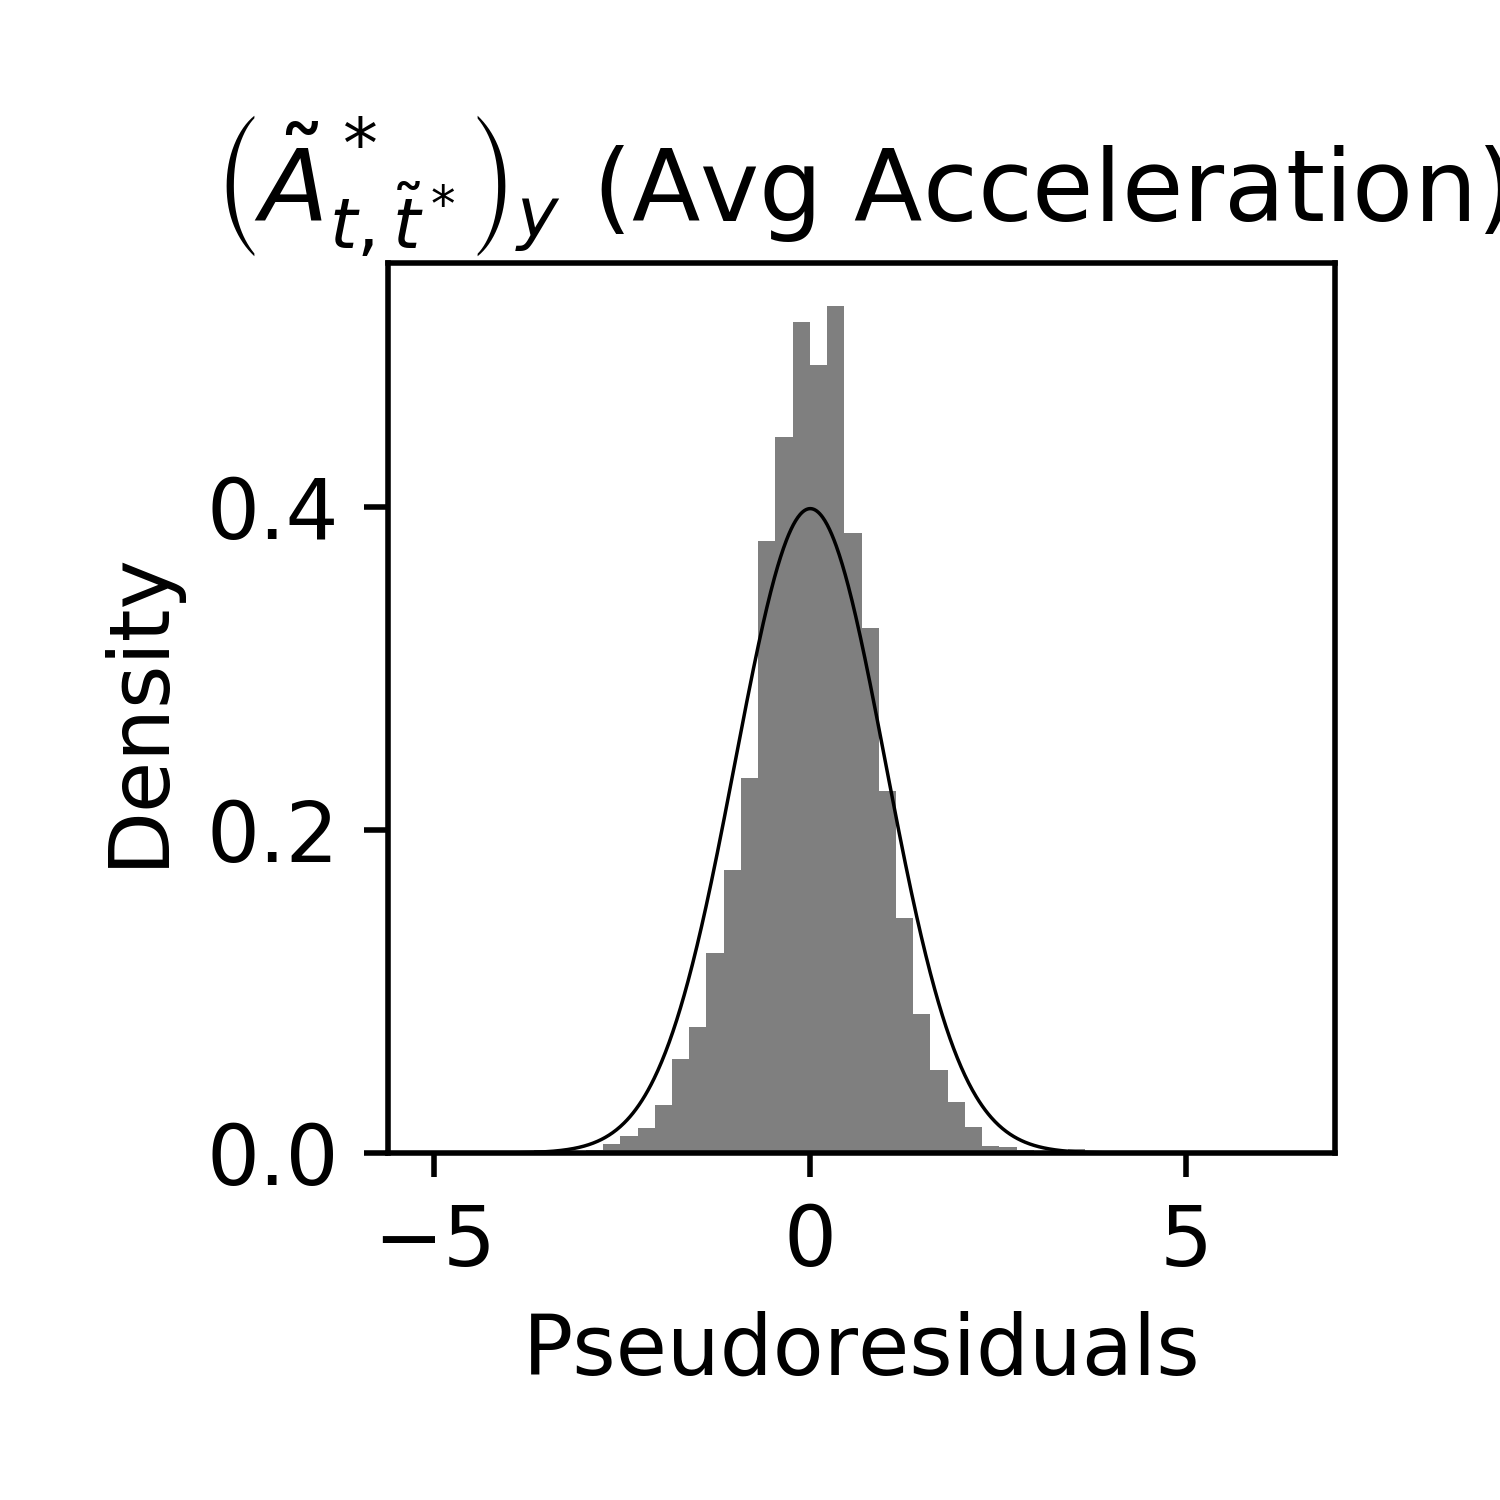
\includegraphics[width=1.75in]{../Plots/HHMM_psedoresids_Ay.png}
        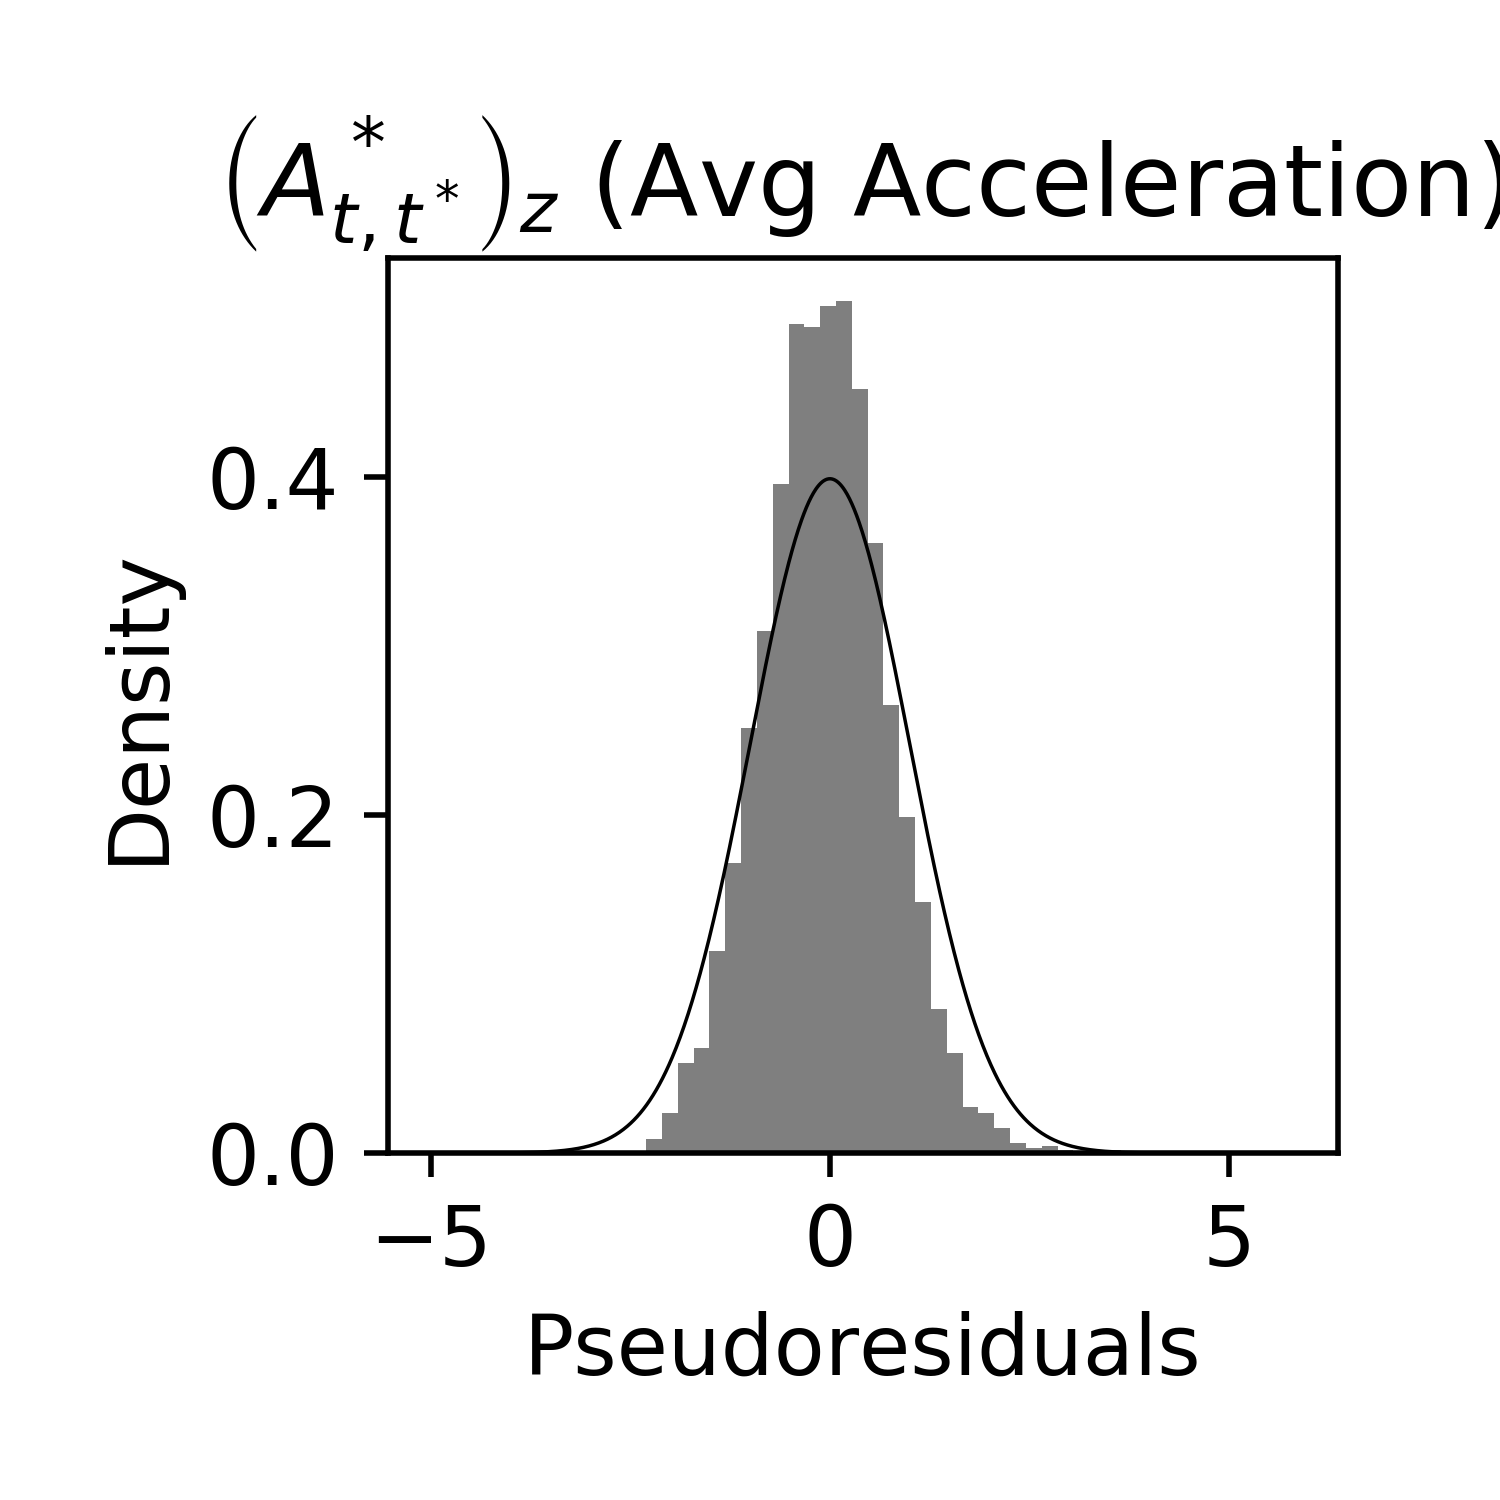
\includegraphics[width=1.75in]{../Plots/HHMM_psedoresids_Az.png}
        \end{center}
        
        \noindent Figure \arabic{fignum}: Empirical histograms (top three rows) and psuedoresiduals (bottom row) of acceleration ($\Zone_{t,t^*}$) plotted over the learned emission distributions and a standard normal density, respectively. All plots are generated using the fitted HHMM-DFT and the killer whale case study data.
        \addtocounter{fignum}{1}
        
        \newpage
        
        \subsubsection{CarHHMM}
        
        \begin{center}
        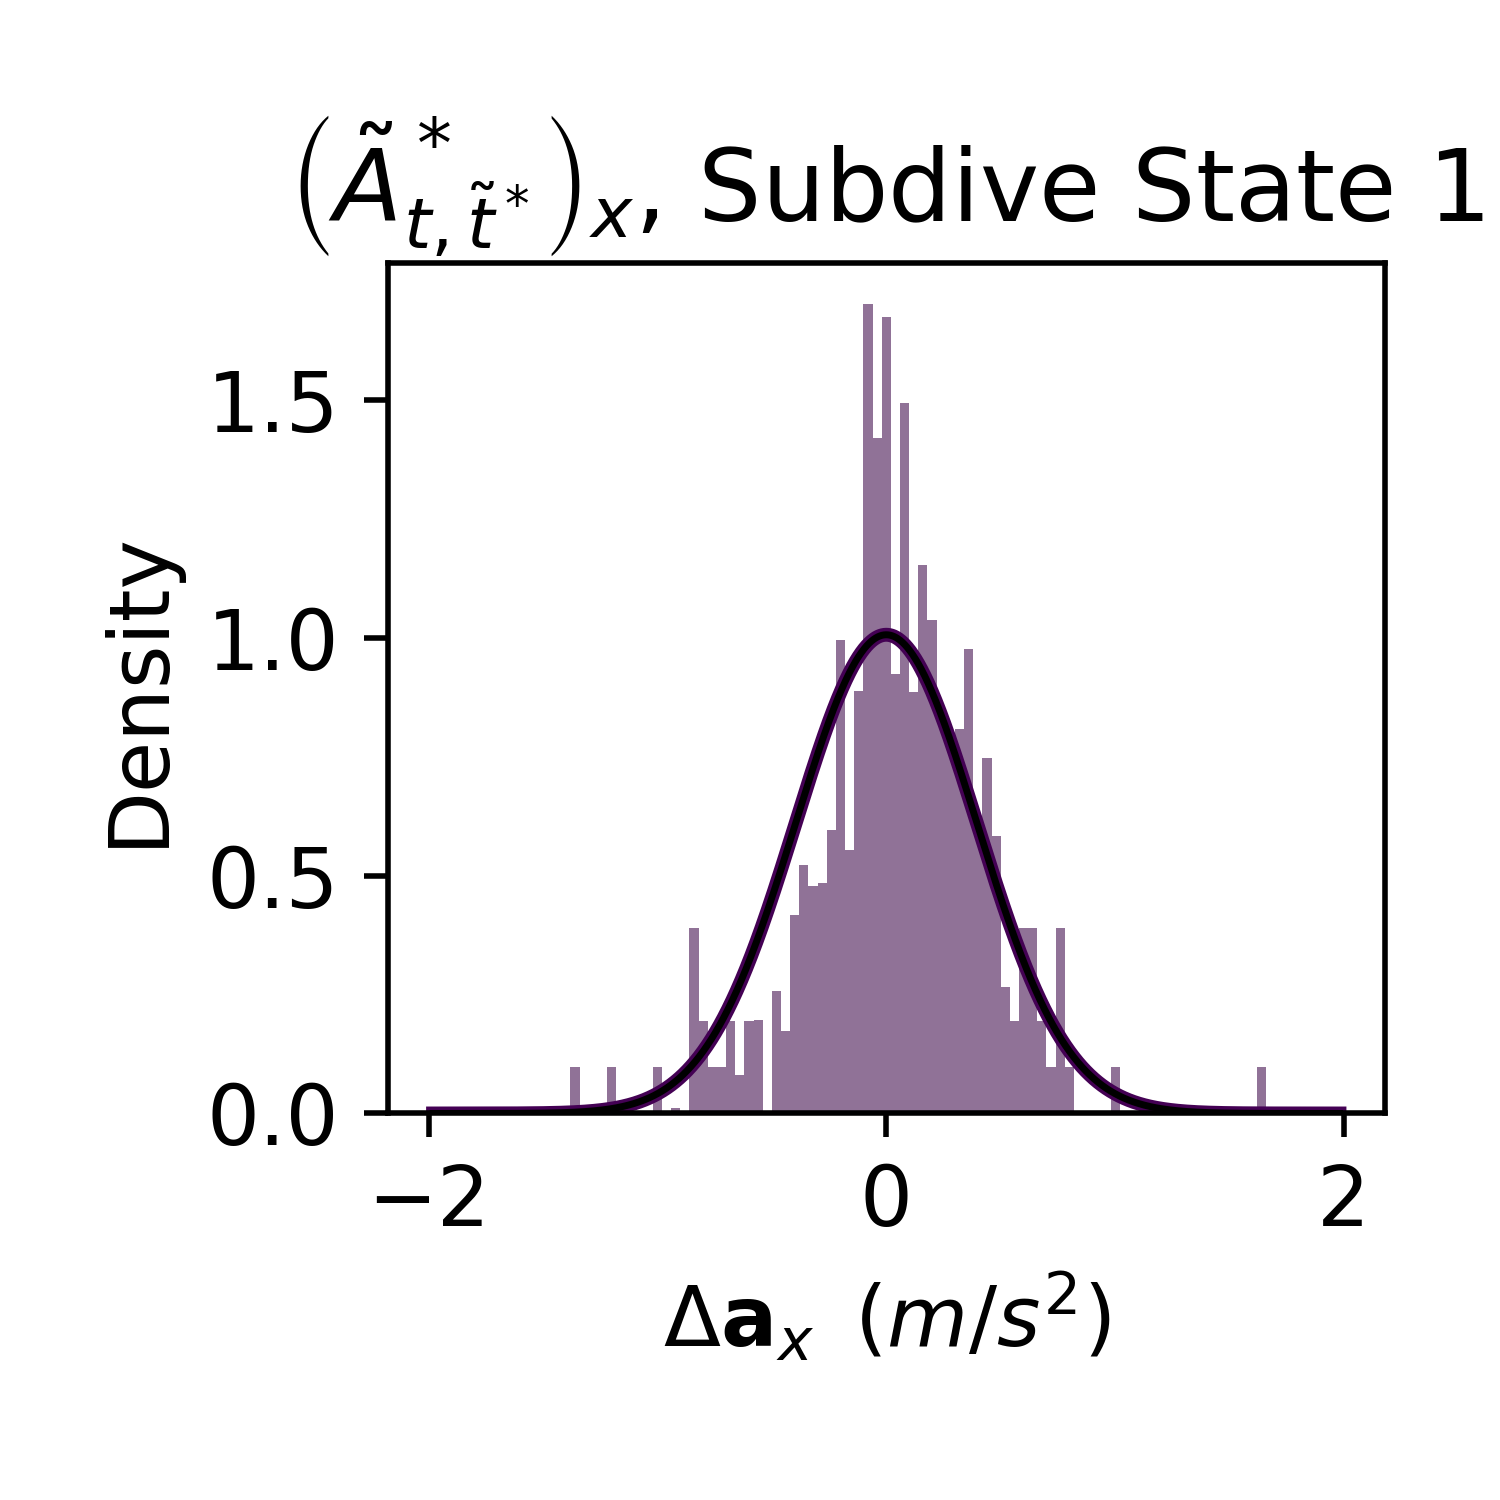
\includegraphics[width=1.75in]{../Plots/CarHHMM1_empirical_hist_Ax_0.png}
        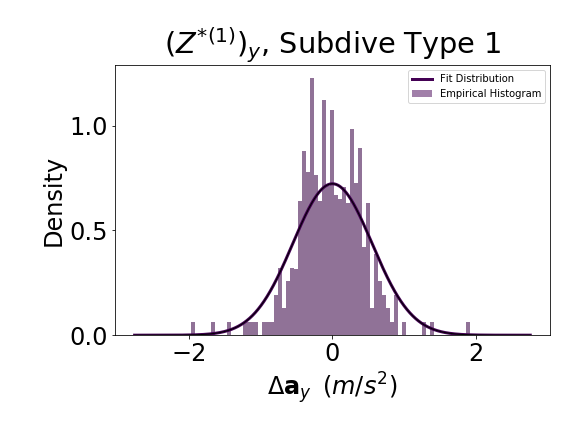
\includegraphics[width=1.75in]{../Plots/CarHHMM1_empirical_hist_Ay_0.png}
        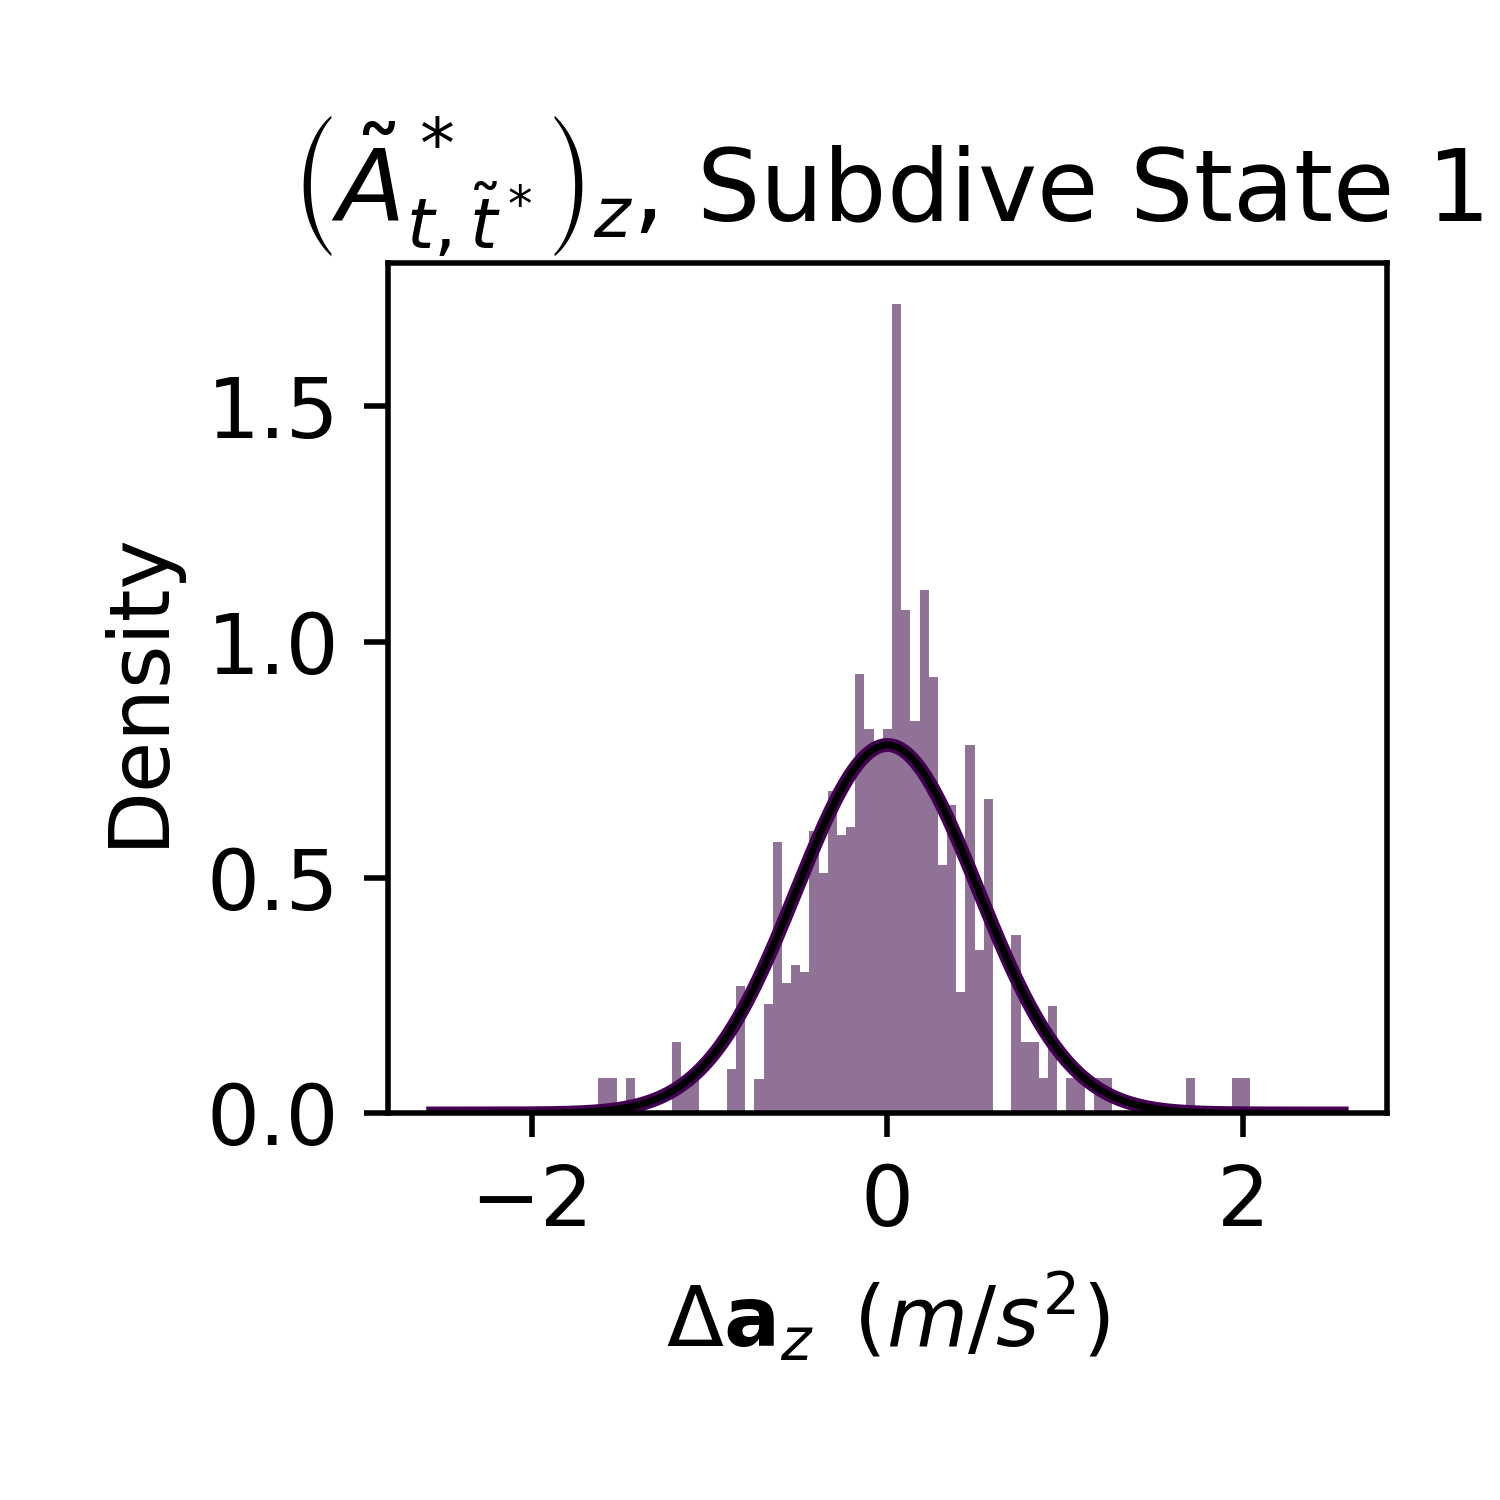
\includegraphics[width=1.75in]{../Plots/CarHHMM1_empirical_hist_Az_0.png}
        
        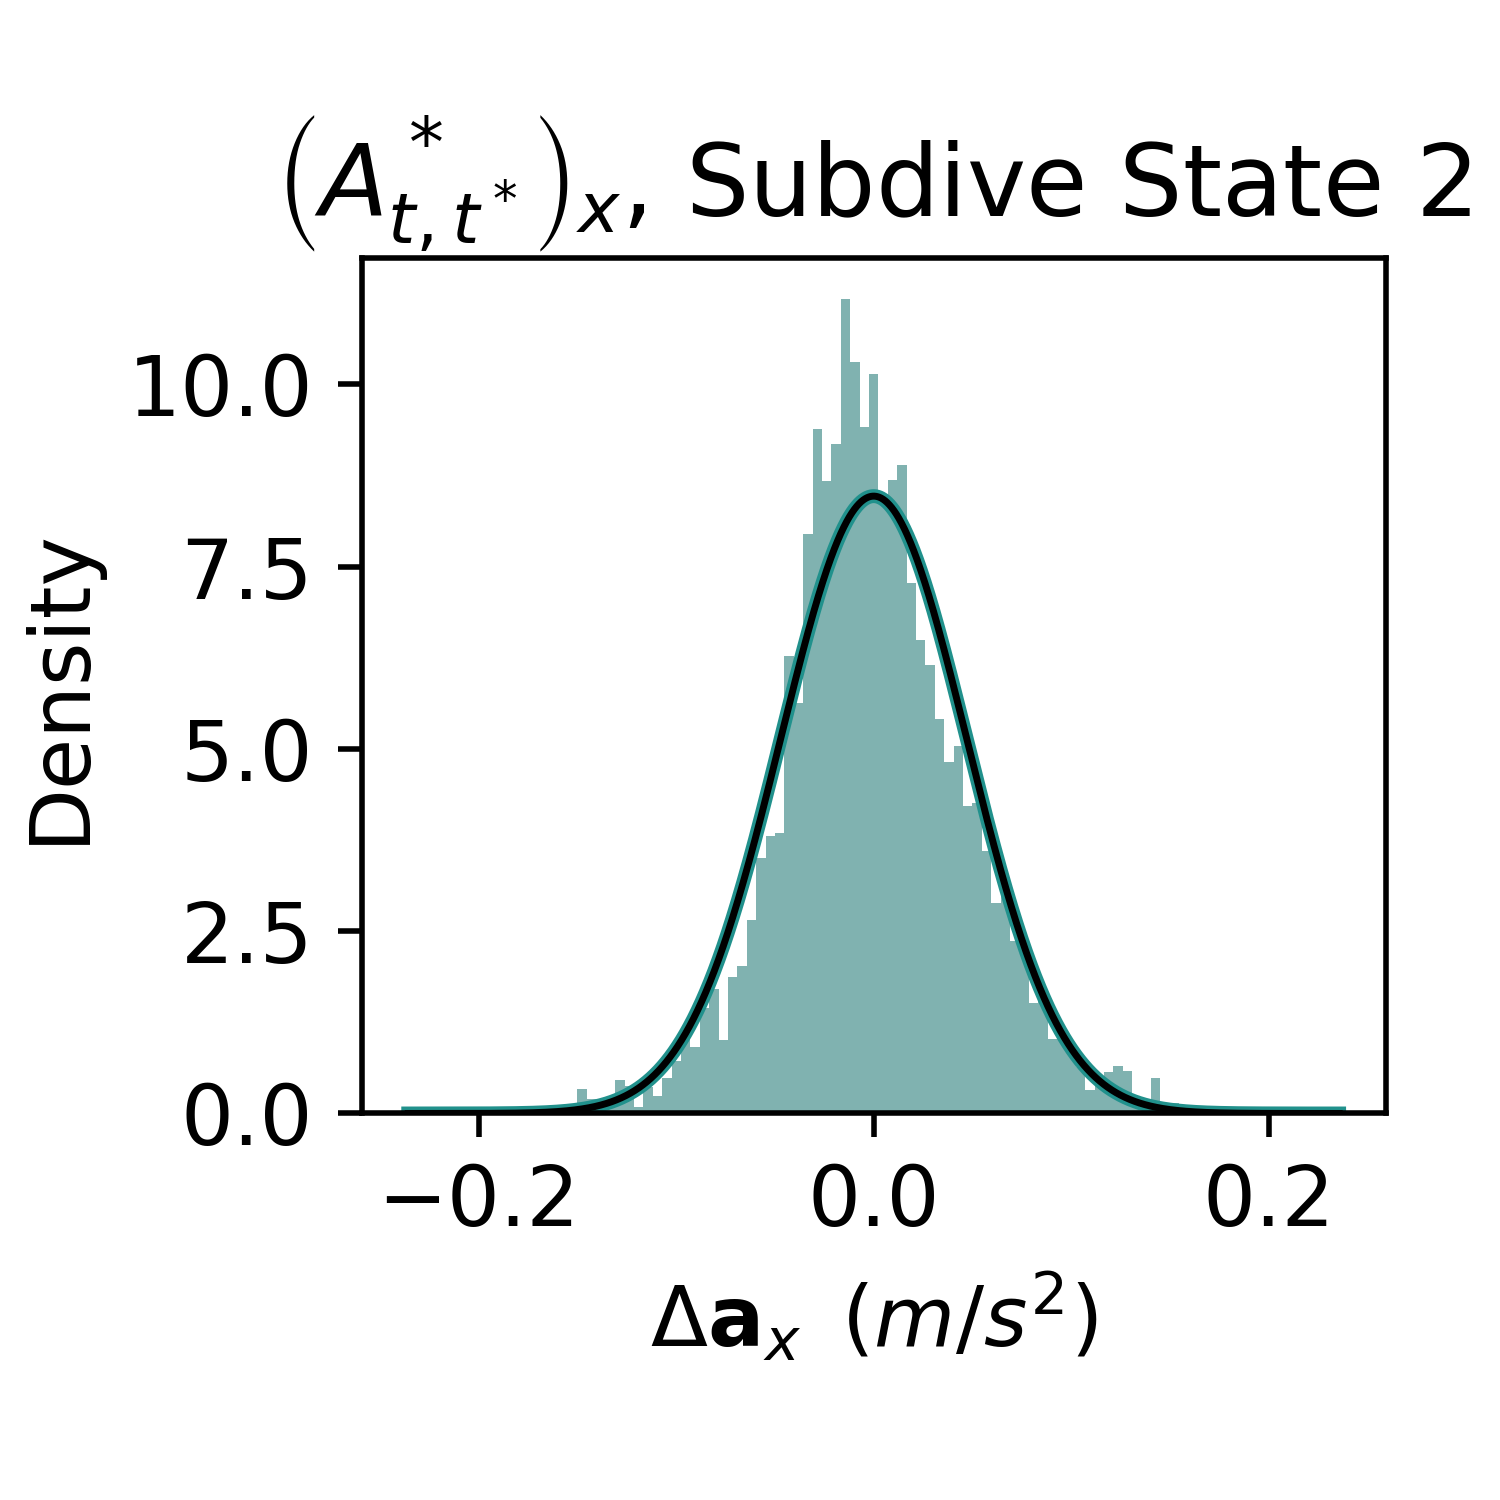
\includegraphics[width=1.75in]{../Plots/CarHHMM1_empirical_hist_Ax_1.png}
        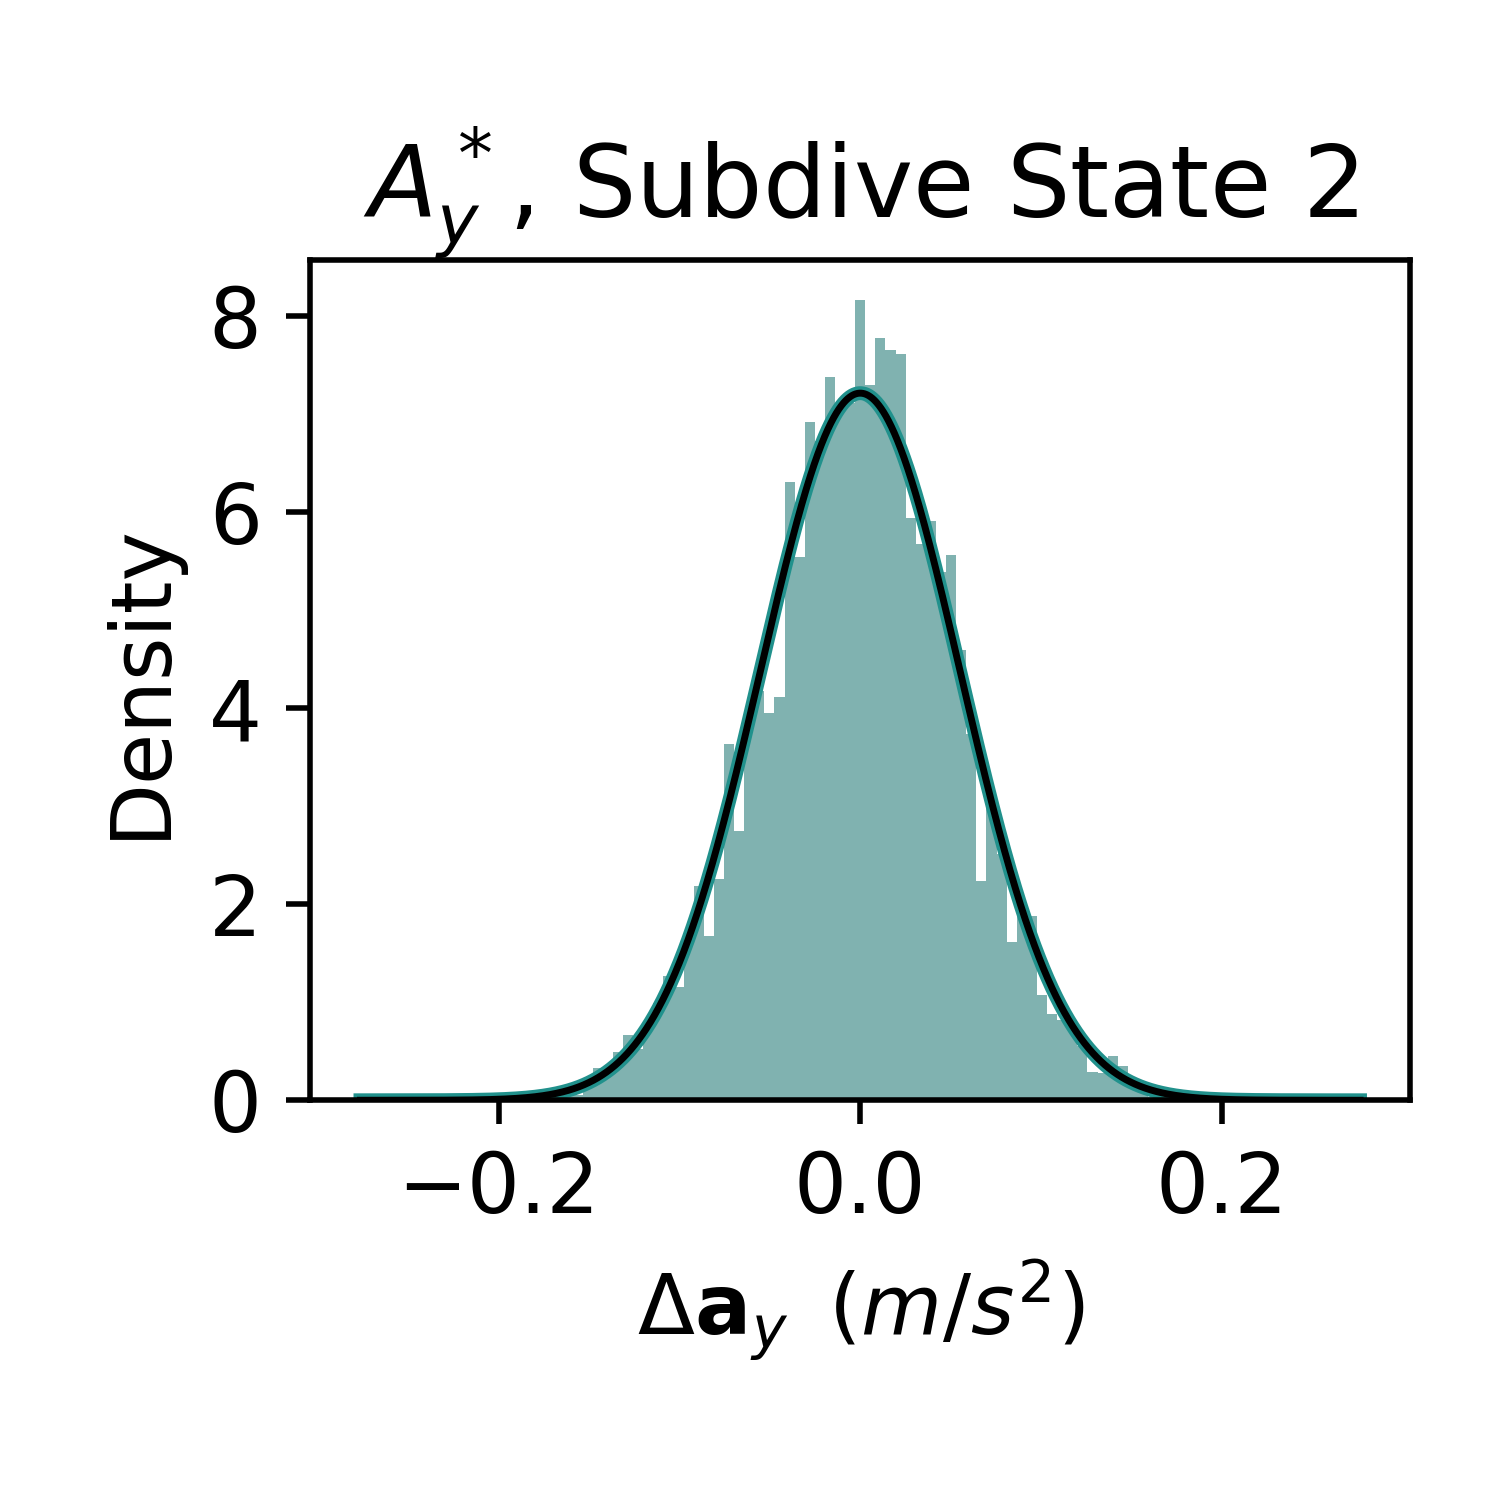
\includegraphics[width=1.75in]{../Plots/CarHHMM1_empirical_hist_Ay_1.png}
        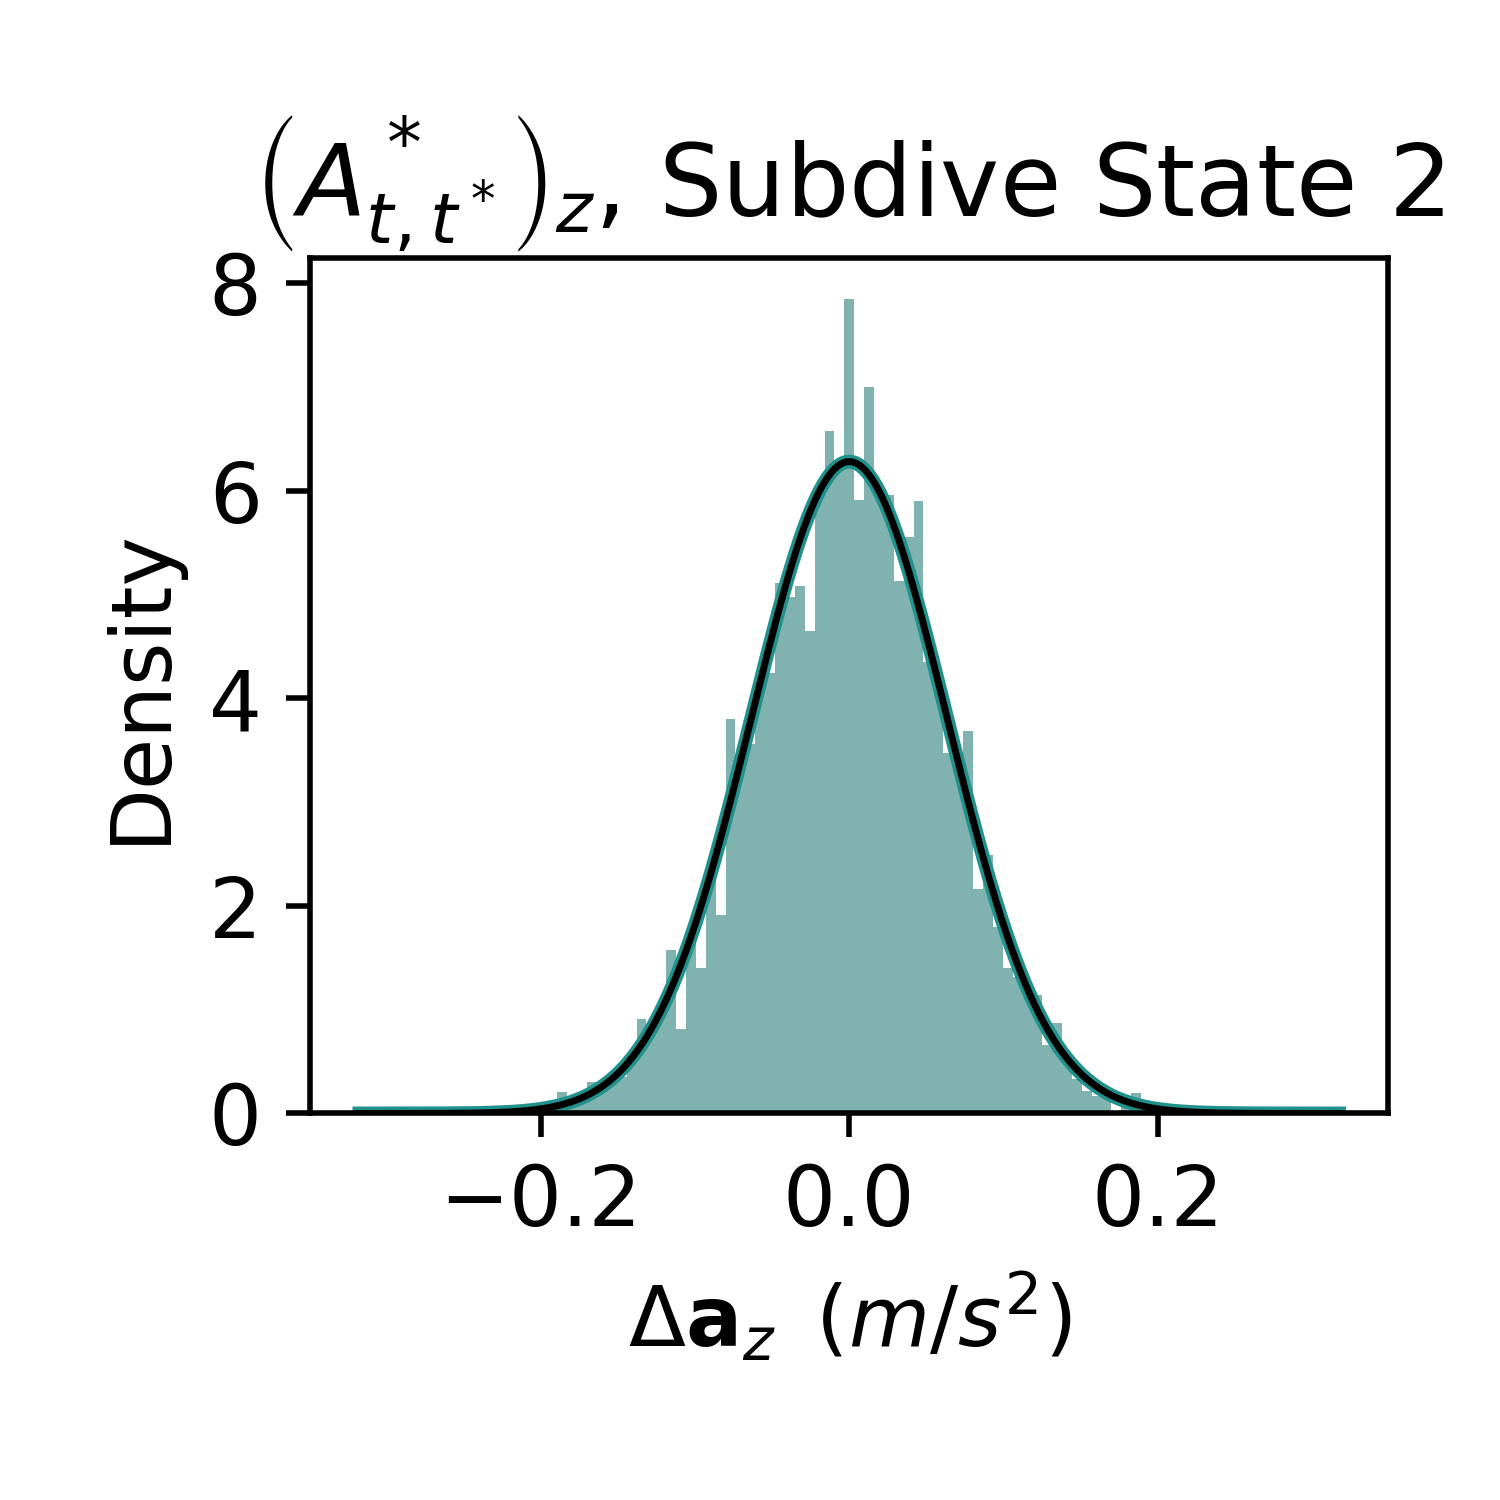
\includegraphics[width=1.75in]{../Plots/CarHHMM1_empirical_hist_Az_1.png}
        
        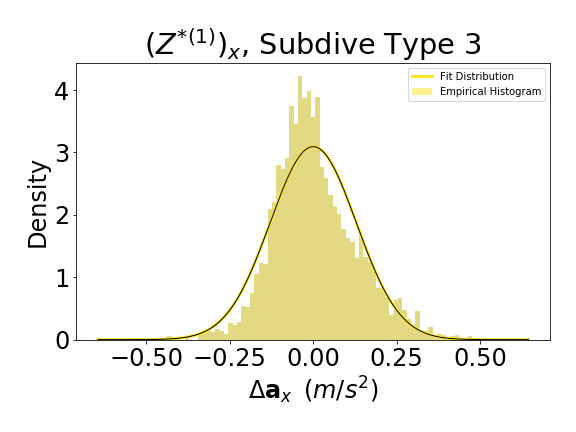
\includegraphics[width=1.75in]{../Plots/CarHHMM1_empirical_hist_Ax_2.png}
        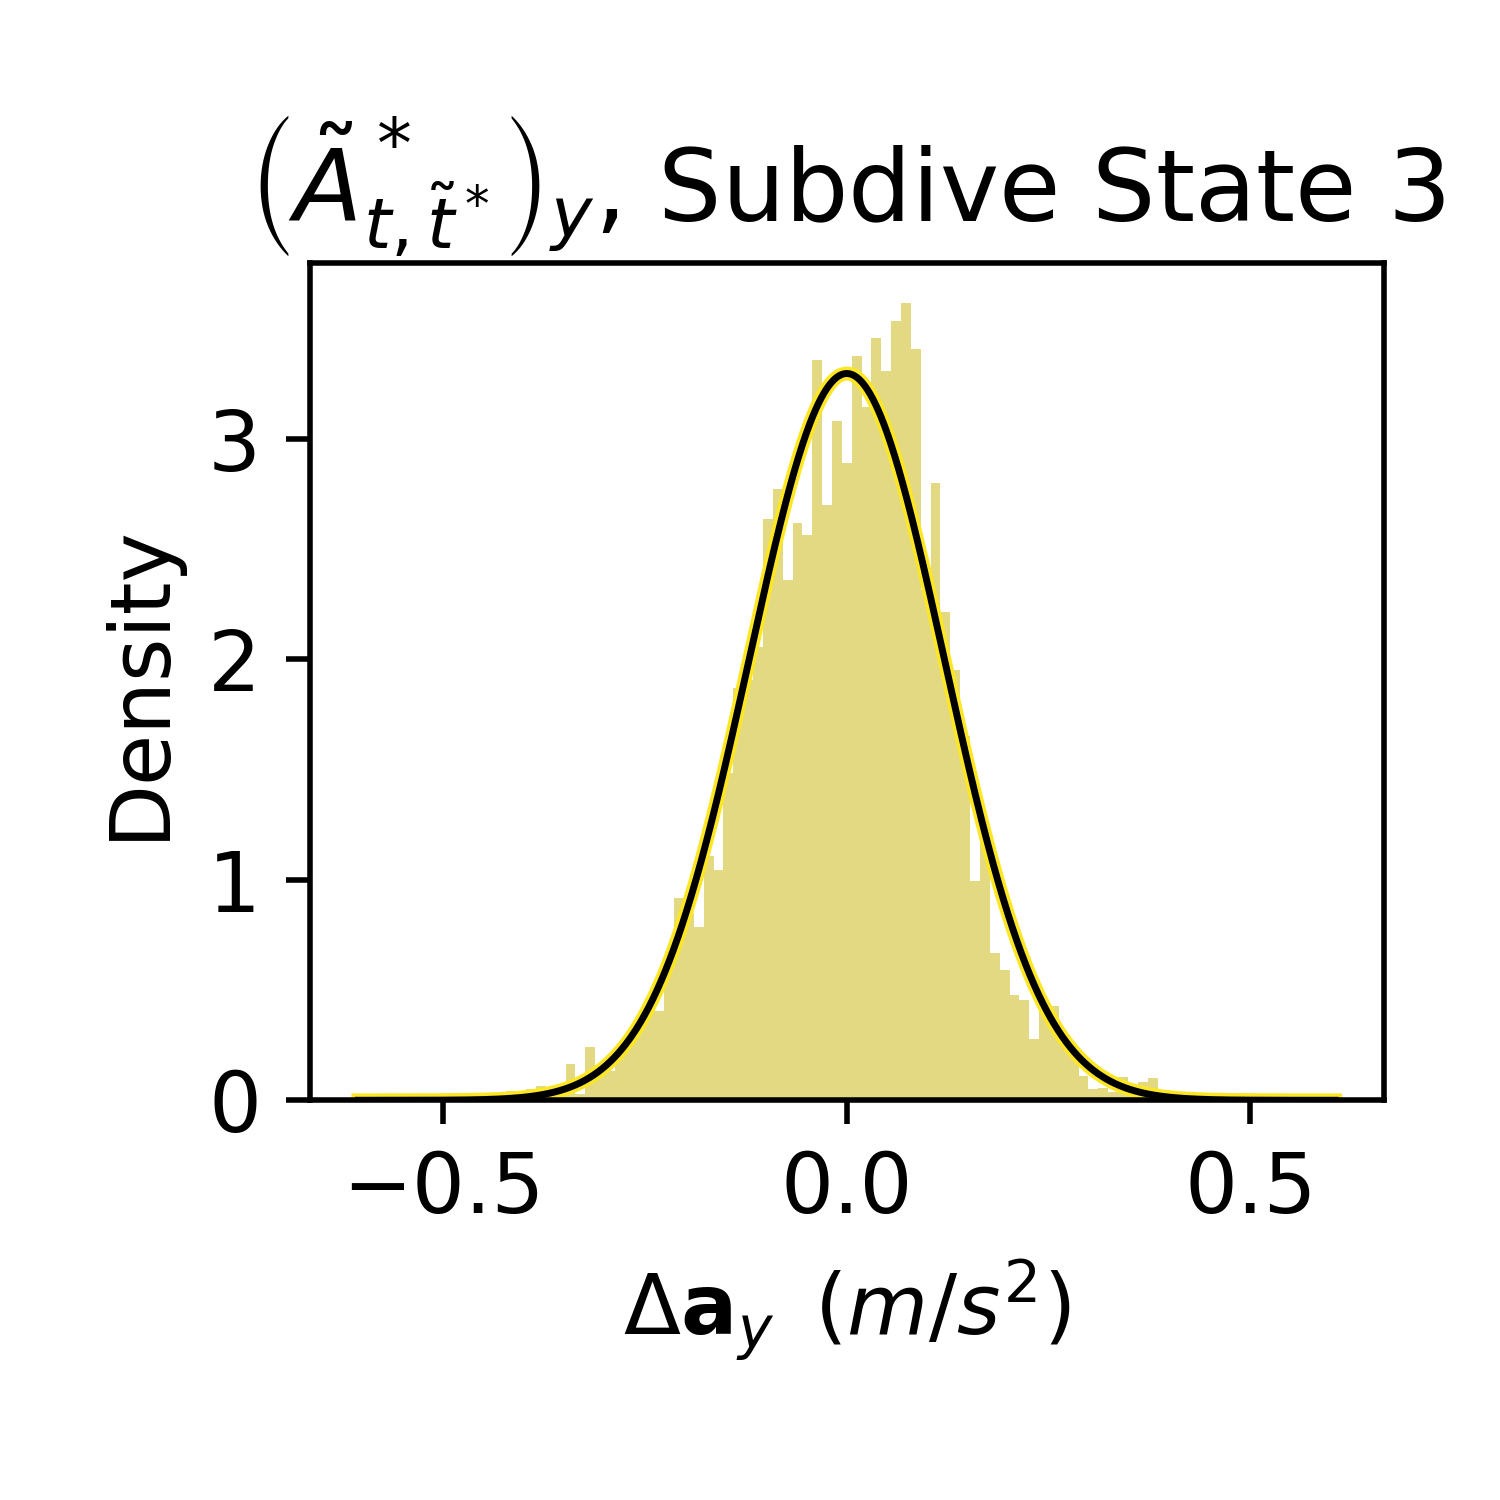
\includegraphics[width=1.75in]{../Plots/CarHHMM1_empirical_hist_Ay_2.png}
        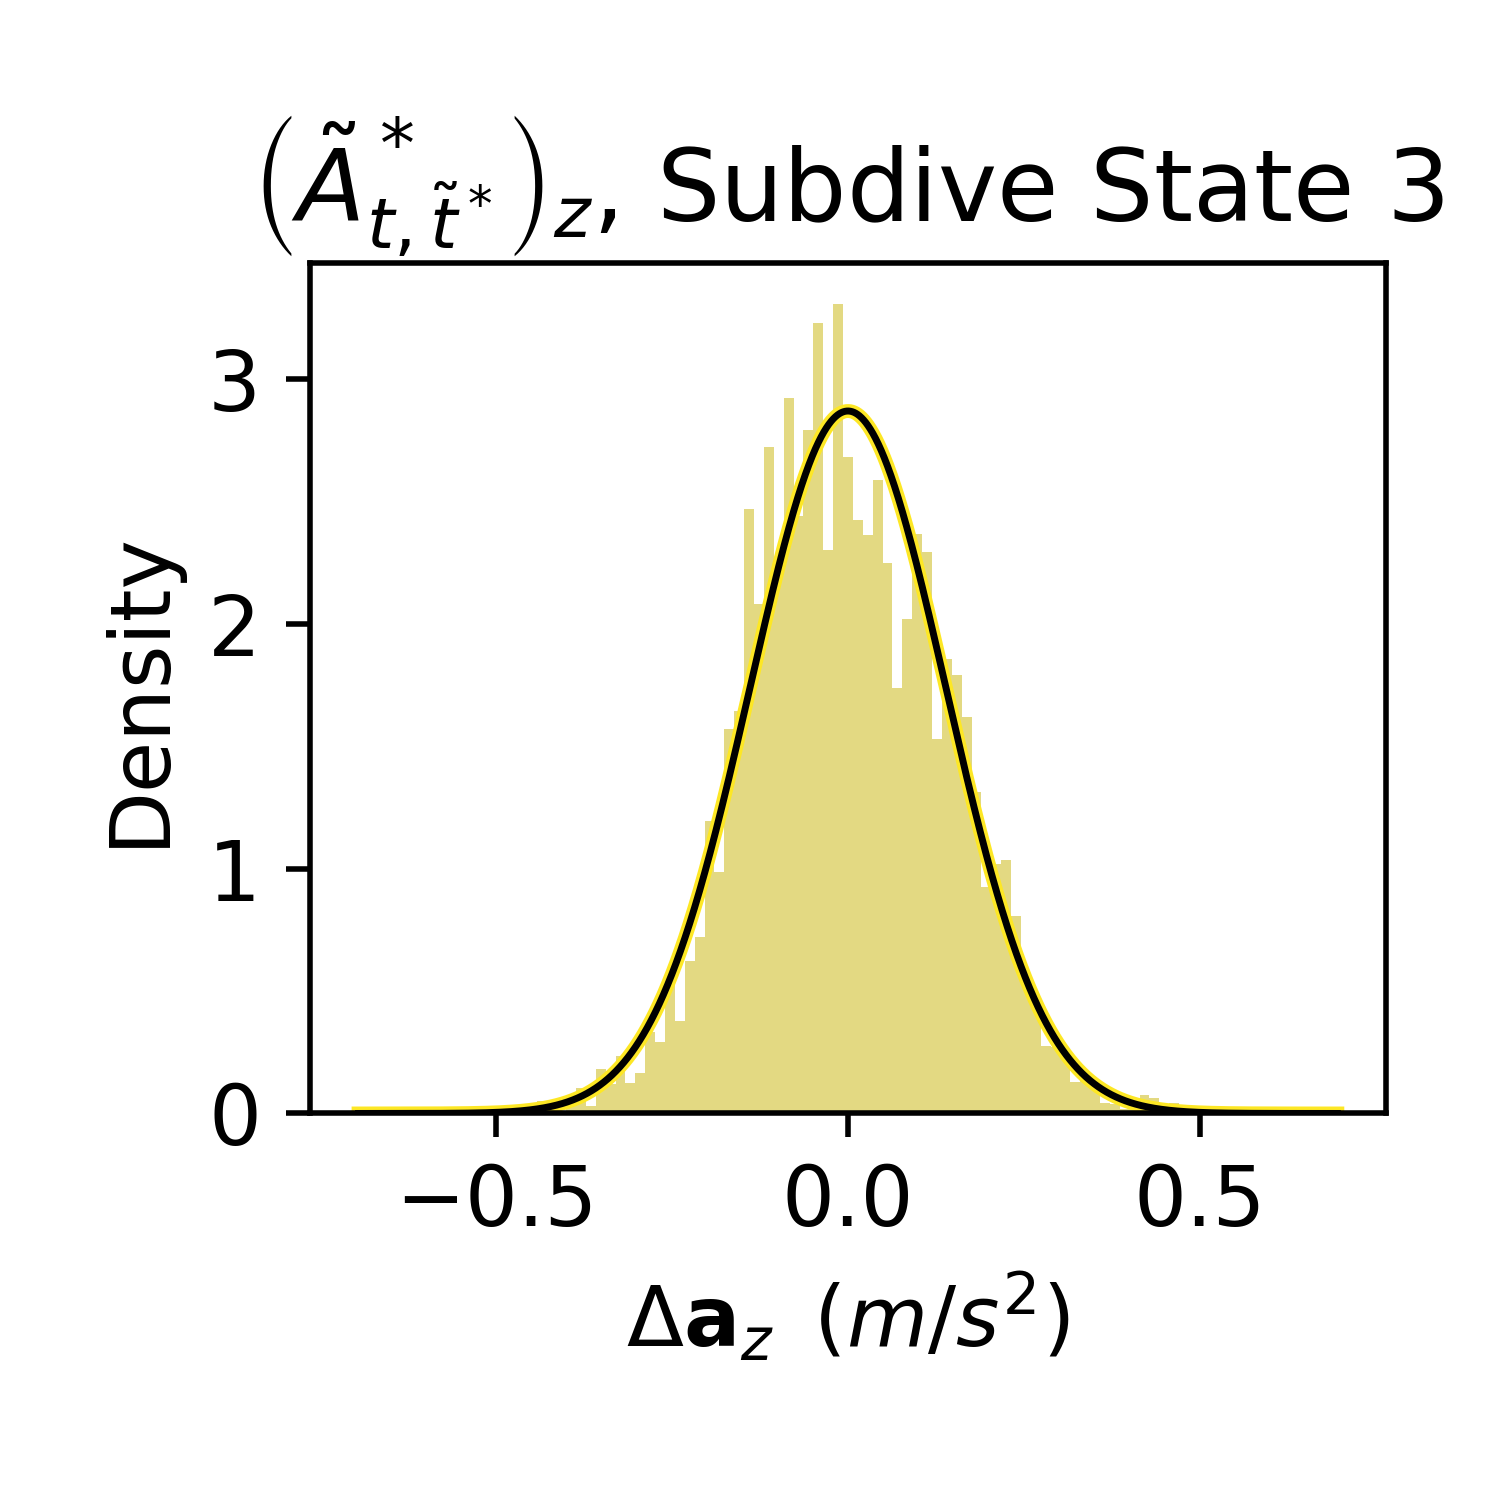
\includegraphics[width=1.75in]{../Plots/CarHHMM1_empirical_hist_Az_2.png}
        
        \includegraphics[width=1.75in]{../Plots/CarHHMM1_psedoresids_Ax.png}
        \includegraphics[width=1.75in]{../Plots/CarHHMM1_psedoresids_Ay.png}
        \includegraphics[width=1.75in]{../Plots/CarHHMM1_psedoresids_Az.png}
        \end{center}
        
        \noindent Figure \arabic{fignum}: Empirical histograms (top three rows) and psuedoresiduals (bottom row) of acceleration ($\Zone_{t,t^*}$) plotted over the learned emission distributions and a standard normal density, respectively. Note that the mean of acceleration at time $t^*$ depends upon acceleration at time $t^*-1$, so only the deviation from the mean for each particular time step is plotted. All plots are generated using the fitted CarHHMM and the killer whale case study data.
        \addtocounter{fignum}{1}
        
        \newpage
        
        \subsubsection{CarHMM-DFT}
        
        \begin{center}
        \includegraphics[width=1.75in]{../Plots/CarHMM_empirical_hist_Ax_0.png}
        \includegraphics[width=1.75in]{../Plots/CarHMM_empirical_hist_Ay_0.png}
        \includegraphics[width=1.75in]{../Plots/CarHMM_empirical_hist_Az_0.png}
        
        \includegraphics[width=1.75in]{../Plots/CarHMM_empirical_hist_Ax_1.png}
        \includegraphics[width=1.75in]{../Plots/CarHMM_empirical_hist_Ay_1.png}
        \includegraphics[width=1.75in]{../Plots/CarHMM_empirical_hist_Az_1.png}
        
        \includegraphics[width=1.75in]{../Plots/CarHMM_empirical_hist_Ax_2.png}
        \includegraphics[width=1.75in]{../Plots/CarHMM_empirical_hist_Ay_2.png}
        \includegraphics[width=1.75in]{../Plots/CarHMM_empirical_hist_Az_2.png}
        
        \includegraphics[width=1.75in]{../Plots/CarHMM_psedoresids_Ax.png}
        \includegraphics[width=1.75in]{../Plots/CarHMM_psedoresids_Ay.png}
        \includegraphics[width=1.75in]{../Plots/CarHMM_psedoresids_Az.png}
        \end{center}
        
        \noindent Figure \arabic{fignum}: Empirical histograms (top three rows) and psuedoresiduals (bottom row) of acceleration ($\Zone_{t,t^*}$) plotted over the learned emission distributions and a standard normal density, respectively. Note that the mean of acceleration at time $t^*$ depends upon acceleration at time $t^*-1$, so only the deviation from the mean for each particular time step is plotted. All plots are generated using the fitted CarHMM-DFT and the killer whale case study data.
        \addtocounter{fignum}{1}
        
    \subsection{Model checking - wiggliness ($\Ztwo_{t,t^*}$)}
        
        \subsubsection{CarHHMM-DFT}
        
        \begin{center}
        \includegraphics[width=1.75in]{../Plots/CarHHMM2_empirical_hist_ahat_0.png}
        \includegraphics[width=1.75in]{../Plots/CarHHMM2_empirical_hist_ahat_1.png}
        \includegraphics[width=1.75in]{../Plots/CarHHMM2_empirical_hist_ahat_2.png}
        
        \includegraphics[width=1.75in]{../Plots/CarHHMM2_psedoresids_ahat.png}
        \end{center}
        
        \noindent Figure \arabic{fignum}: Empirical histograms (top row) and psuedoresiduals (bottom row) of wiggliness ($\Ztwo_{t,t^*}$) plotted over the learned emission distributions and a standard normal density, respectively. All plots are generated using the fitted CarHHMM-DFT and the killer whale case study data.
        \addtocounter{fignum}{1}
        
        \subsubsection{HHMM-DFT}
        
        \begin{center}
        \includegraphics[width=1.75in]{../Plots/HHMM_empirical_hist_ahat_0.png}
        \includegraphics[width=1.75in]{../Plots/HHMM_empirical_hist_ahat_1.png}
        \includegraphics[width=1.75in]{../Plots/HHMM_empirical_hist_ahat_2.png}
        
        \includegraphics[width=1.75in]{../Plots/HHMM_psedoresids_ahat.png}
        \end{center}
        
        \noindent Figure \arabic{fignum}: Empirical histograms (top row) and psuedoresiduals (bottom row) of wiggliness ($\Ztwo_{t,t^*}$) plotted over the learned emission distributions and a standard normal density, respectively. All plots are generated using the fitted HHMM-DFT and the killer whale case study data.
        \addtocounter{fignum}{1}
        
        \subsubsection{CarHHMM}
        
        The CarHHMM does not model wiggliness.
        
        \subsubsection{CarHMM-DFT}
        
        \begin{center}
        \includegraphics[width=1.75in]{../Plots/CarHMM_empirical_hist_ahat_0.png}
        \includegraphics[width=1.75in]{../Plots/CarHMM_empirical_hist_ahat_1.png}
        \includegraphics[width=1.75in]{../Plots/CarHMM_empirical_hist_ahat_2.png}
        
        \includegraphics[width=1.75in]{../Plots/CarHMM_psedoresids_ahat.png}
        \end{center}
        
        \noindent Figure \arabic{fignum}: Empirical histograms (top row) and psuedoresiduals (bottom row) of wiggliness ($\Ztwo_{t,t^*}$) plotted over the learned emission distributions and a standard normal density, respectively. All plots are generated using the fitted CarHMM-DFT and the killer whale case study data.
        \addtocounter{fignum}{1}


\newpage
\section{Simulation Study Results}

    \subsection{Accuracy comparisons}
        
        \begin{center}
        \scalebox{0.75}{
        \bgroup
        \def\arraystretch{1.5}
        \begin{tabular}{ccccccc}
        Model                       & \multicolumn{1}{c}{Train Time (m)} & \multicolumn{1}{c}{Dive Type} & \multicolumn{1}{c}{Subdive Type} & \multicolumn{1}{c}{Dive Accuracy} & \multicolumn{1}{c}{Subdive Accuracy}    \\ \hline
        \multirow{5}{*}{CarHHMM-DFT}& \multirow{5}{*}{$150 \pm 37$}      & Both                          & Both                             & $0.936 \pm 0.025$                 & $1.000 \pm 0.000$                       \\
                                    &                                    & 1                             & 1                                & \multirow{2}{*}{$0.933\pm0.036$}  & $1.000 \pm 0.000$                       \\ 
                                    &                                    & 1                             & 2                                &                                   & $1.000 \pm 0.000$                       \\ 
                                    &                                    & 2                             & 1                                & \multirow{2}{*}{$0.940\pm0.034$}  & $1.000 \pm 0.000$                       \\ 
                                    &                                    & 2                             & 2                                &                                   & $1.000 \pm 0.000$                       \\ \hline
        \multirow{5}{*}{HHMM-DFT}   & \multirow{5}{*}{$140 \pm 29$}      & Both                          & Both                             & $0.936 \pm 0.026$                 & $1.000 \pm 0.000$                       \\
                                    &                                    & 1                             & 1                                & \multirow{2}{*}{$0.932\pm0.038$}  & $1.000 \pm 0.000$                       \\ 
                                    &                                    & 1                             & 2                                &                                   & $1.000 \pm 0.000$                       \\ 
                                    &                                    & 2                             & 1                                & \multirow{2}{*}{$0.941\pm0.032$}  & $1.000 \pm 0.000$                       \\ 
                                    &                                    & 2                             & 2                                &                                   & $1.000 \pm 0.000$                       \\ \hline
        \multirow{5}{*}{CarHHMM}    & \multirow{5}{*}{$258 \pm 82$}      & Both                          & Both                             & $0.87 \pm 0.11$                   & $0.893 \pm 0.007$                       \\
                                    &                                    & 1                             & 1                                & \multirow{2}{*}{$0.79\pm0.23$}    & $0.428 \pm 0.085$                       \\ 
                                    &                                    & 1                             & 2                                &                                   & $1.000 \pm 0.000$                       \\ 
                                    &                                    & 2                             & 1                                & \multirow{2}{*}{$0.955\pm0.034$}  & $0.816 \pm 0.014$                       \\ 
                                    &                                    & 2                             & 2                                &                                   & $1.000 \pm 0.001$                       \\ \hline
        \multirow{5}{*}{CarHMM-DFT} & \multirow{5}{*}{$62 \pm 10$}       & Both                          & Both                             & -------------                     & $1.000 \pm 0.000$                       \\
                                    &                                    & 1                             & 1                                & \multirow{2}{*}{-------------}    & $1.000 \pm 0.000$                       \\ 
                                    &                                    & 1                             & 2                                &                                   & $1.000 \pm 0.000$                       \\ 
                                    &                                    & 2                             & 1                                & \multirow{2}{*}{-------------}    & $1.000 \pm 0.000$                       \\ 
                                    &                                    & 2                             & 2                                &                                   & $1.000 \pm 0.000$                       \\ \hline 
        \end{tabular}
        \egroup
        }
        \end{center}
        
        \noindent Table \arabic{tablenum}: Accuracies and run times for all models in the simulation study. All reported values are averages, and $\pm$ refers to the standard deviation across a total of 500 fitted models. Both training and test data sets are made up of 100 simulated dives. Rows labelled Both/Both correspond to overall model accuracy.
        \addtocounter{tablenum}{1}

    \newpage
    \subsection{Empirical joint distributions - dive duration ($Y_t$)}

        \begin{center}
        \scalebox{0.75}{
        \bgroup
        \centering
        \def\arraystretch{1.5}
        \begin{tabular}{ccccccc}
        Model                       & \multicolumn{1}{c}{Parameter} & \multicolumn{1}{c}{Dive Type} & \multicolumn{1}{c}{Estimate}   & \multicolumn{1}{c}{Bias}   & \multicolumn{1}{c}{Empirical SE}    & \multicolumn{1}{c}{Observed Fischer SE}     \\ \hline
        \multirow{4}{*}{CarHHMM-DFT}& \multirow{2}{*}{$\mu$}        & 1                             & $19.988$                       & $-0.012$ $(p=0.726)$       & $0.759$                             & $0.681 \pm 0.114$                           \\
                                    &                               & 2                             & $80.311$                       & $0.311$ $(p=0.415)$        & $8.498$                             & $5.858 \pm 1.178$                           \\
                                    & \multirow{2}{*}{$\sigma$}     & 1                             & $4.901$                        & $-0.099$ $(p=0.000)$       & $0.626$                             & $0.528 \pm 0.097$                           \\
                                    &                               & 2                             & $48.405$                       & $-1.595$ $(p=0.000)$       & $6.645$                             & $5.105 \pm 1.004$                           \\ \hline
        \multirow{4}{*}{HHMM-DFT}   & \multirow{2}{*}{$\mu$}        & 1                             & $19.989$                       & $-0.011$ $(p=0.757)$       & $0.759$                             & $0.684 \pm 0.113$                           \\
                                    &                               & 2                             & $80.309$                       & $0.309$ $(p=0.418)$        & $8.488$                             & $5.853 \pm 1.167$                           \\
                                    & \multirow{2}{*}{$\sigma$}     & 1                             & $4.902$                        & $-0.098$ $(p=0.000)$       & $0.626$                             & $0.529 \pm 0.097$                           \\
                                    &                               & 2                             & $48.398$                       & $-1.602$ $(p=0.000)$       & $6.638$                             & $5.104 \pm 1.019$                           \\ \hline
        \multirow{4}{*}{CarHHMM}    & \multirow{2}{*}{$\mu$}        & 1                             & $21.130$                       & $1.130$ $(p=0.000)$        & $5.698$                             & $0.704 \pm 0.150$                           \\
                                    &                               & 2                             & $74.877$                       & $-5.123$ $(p=0.000)$       & $10.784$                            & $5.236 \pm 1.463$                           \\
                                    & \multirow{2}{*}{$\sigma$}     & 1                             & $4.487$                        & $-0.513$ $(p=0.000)$       & $1.297$                             & $0.556 \pm 0.134$                           \\
                                    &                               & 2                             & $47.808$                       & $-2.192$ $(p=0.000)$       & $6.737$                             & $4.731 \pm 1.121$                           \\ \hline
        \multirow{4}{*}{CarHMM-DFT} & \multirow{2}{*}{$\mu$}        & 1                             & $49.976$                       & $-0.024$ $(p=0.911)$       & $4.710$                             & $2.479 \pm 0.343$                           \\
                                    &                               & ---                           & ---                            & ---                        & ---                                 & ---                                         \\
                                    & \multirow{2}{*}{$\sigma$}     & 1                             & $39.210$                       & $-7.293$ $(p=0.000)$       & $5.001$                             & $2.516 \pm 0.405$                           \\
                                    &                               & ---                           & ---                            & ---                        & ---                                 & ---                                         \\ \hline
        \end{tabular}
        \egroup
        }
        \end{center}
        
        \noindent Table \arabic{tablenum}: Estimates and standard errors for the parameters of the distribution of dive duration across all four models. The ``estimate" column is the average across 500 simulations, and the ``observed Fisher standard error" column is the median across 500 simulations. The $\pm$ refers to the inter-quartile range. SE stands for standard error. Reported p-values test if the observed bias is statistically significant using a one-sample $t$-test.
        \addtocounter{tablenum}{1}
        
        \subsubsection{CarHHMM-DFT}
        \begin{center}
        \includegraphics[width=3in]{../Plots/hhmm_FV_MLE_density_dive_duration_-1_0.png}
        \includegraphics[width=3in]{../Plots/hhmm_FV_MLE_density_dive_duration_-1_1.png}
        \end{center}
        
        \noindent Figure \arabic{fignum}: Kernel density estimate of the distribution of estimates of dive duration parameters ($\hat \mu_Y$ and $\hat \sigma_Y$) for each dive type. The red star represents the true values of $\mu_Y$ and $\sigma_Y$ for both dive types. These estimates are for the CarHHMM-DFT.
        \addtocounter{fignum}{1}
        
        \subsubsection{HHMM-DFT}
        \begin{center}
        \includegraphics[width=3in]{../Plots/hhmm_FV_uncorr_MLE_density_dive_duration_-1_0.png}
        \includegraphics[width=3in]{../Plots/hhmm_FV_uncorr_MLE_density_dive_duration_-1_1.png}
        \end{center}

        \noindent Figure \arabic{fignum}: Kernel density estimate of the distribution of estimates of dive duration parameters ($\hat \mu_Y$ and $\hat \sigma_Y$) for each dive type. The red star represents the true values of $\mu_Y$ and $\sigma_Y$ for both dive types. These estimates are for the HHMM-DFT.
        \addtocounter{fignum}{1}
        
        \subsubsection{CarHHMM}
        \begin{center}
        \includegraphics[width=3in]{../Plots/hhmm_V_MLE_density_dive_duration_-1_0.png}
        \includegraphics[width=3in]{../Plots/hhmm_V_MLE_density_dive_duration_-1_1.png}
        \end{center}
        
        \noindent Figure \arabic{fignum}: Kernel density estimate of the distribution of estimates of dive duration parameters ($\hat \mu_Y$ and $\hat \sigma_Y$) for each dive type. The red star represents the true values of $\mu_Y$ and $\sigma_Y$ for both dive types. These estimates are for the CarHHMM.
        \addtocounter{fignum}{1}
        
        \subsubsection{CarHMM-DFT}
        \begin{center}
        \includegraphics[width=3in]{../Plots/hmm_FV_MLE_density_dive_duration_-1_0.png}
        \end{center}
        
        \noindent Figure \arabic{fignum}: Kernel density estimate of the distribution of estimates of dive duration parameters ($\hat \mu_Y$ and $\hat \sigma_Y$) for each dive type. The red star represents the true values of $\mu_Y$ and $\sigma_Y$ for both dive types. These estimates are for the CarHMM-DFT. The CarHMM-DFT assumes that there is only one dive type, so we have that $\Gamma = \begin{pmatrix} 1 \end{pmatrix}$, and there is only one version of the fine scale probability transition matrix $\Gamma^*$ (see Table 9).
    
    \newpage
    \subsection{Empirical joint distributions - acceleration ($\Zone_{t,t^*}$)}

        \begin{center}
        \scalebox{0.75}{
        \bgroup
        \centering
        \def\arraystretch{1.5}
        \begin{tabular}{ccccccc}
        Model                       & \multicolumn{1}{c}{Parameter} & \multicolumn{1}{c}{Subdive Type} & \multicolumn{1}{c}{Estimate}    & \multicolumn{1}{c}{Bias}     & \multicolumn{1}{c}{Empirical SE}   & \multicolumn{1}{c}{Observed Fischer SE}        \\ \hline
        \multirow{6}{*}{CarHHMM-DFT}& \multirow{2}{*}{$\mu$}        & 1                                & $0.003$                         & $0.003$ $(p=0.675)$          & $0.177$                             & $0.130 \pm 0.116$                             \\
                                    &                               & 2                                & $-0.003$                        & $-0.003$ $(p=0.264)$         & $0.058$                             & $0.056 \pm 0.019$                             \\
                                    & \multirow{2}{*}{$\sigma$}     & 1                                & $0.049$                         & $-0.001$ $(p=0.000)$         & $0.001$                             & $0.001 \pm 0.000$                             \\
                                    &                               & 2                                & $0.097$                         & $-0.003$ $(p=0.000)$         & $0.002$                             & $0.002 \pm 0.000$                             \\ 
                                    & \multirow{2}{*}{$\phi$}       & 1                                & $0.989$                         & $-0.001$ $(p=0.000)$         & $0.006$                             & $0.005 \pm 0.001$                             \\
                                    &                               & 2                                & $0.948$                         & $-0.002$ $(p=0.006)$         & $0.013$                             & $0.012 \pm 0.002$                             \\ \hline
        \multirow{6}{*}{HHMM-DFT}   & \multirow{2}{*}{$\mu$}        & 1                                & $0.001$                         & $0.001$ $(p=0.390)$          & $0.032$                             & $0.007 \pm 0.001$                             \\
                                    &                               & 2                                & $-0.001$                        & $-0.001$ $(p=0.549)$         & $0.024$                             & $0.007 \pm 0.001$                             \\
                                    & \multirow{2}{*}{$\sigma$}     & 1                                & $0.248$                         & $0.198$ $(p=0.000)$          & $0.023$                             & $0.005 \pm 0.001$                             \\
                                    &                               & 2                                & $0.242$                         & $0.142$ $(p=0.000)$          & $0.018$                             & $0.005 \pm 0.000$                             \\ 
                                    & \multirow{2}{*}{$\phi$}       & 1                                & ------                          & ------                       & ------                              & ------                                        \\
                                    &                               & 2                                & ------                          & ------                       & ------                              & ------                                        \\ \hline
        \multirow{6}{*}{CarHHMM}    & \multirow{2}{*}{$\mu$}        & 1                                & $0.004$                         & $0.004$ $(p=0.251)$          & $0.083$                             & $0.080 \pm 0.036$                             \\
                                    &                               & 2                                & $-0.001$                        & $-0.001$ $(p=0.327)$         & $0.024$                             & $0.009 \pm 0.001$                             \\
                                    & \multirow{2}{*}{$\sigma$}     & 1                                & $0.048$                         & $-0.002$ $(p=0.000)$         & $0.001$                             & $0.001 \pm 0.000$                             \\
                                    &                               & 2                                & $0.272$                         & $0.172$ $(p=0.000)$          & $0.005$                             & $0.004 \pm 0.000$                             \\ 
                                    & \multirow{2}{*}{$\phi$}       & 1                                & $0.986$                         & $-0.004$ $(p=0.000)$         & $0.005$                             & $0.004 \pm 0.001$                             \\
                                    &                               & 2                                & $0.428$                         & $-0.522$ $(p=0.000)$         & $0.058$                             & $0.018 \pm 0.001$                             \\ \hline
        \multirow{6}{*}{CarHMM-DFT} & \multirow{2}{*}{$\mu$}        & 1                                & $0.011$                         & $0.011$ $(p=0.339)$          & $0.246$                             & $0.130 \pm 0.118$                             \\
                                    &                               & 2                                & $-0.003$                        & $-0.003$ $(p=0.261)$         & $0.058$                             & $0.056 \pm 0.019$                             \\
                                    & \multirow{2}{*}{$\sigma$}     & 1                                & $0.049$                         & $-0.001$ $(p=0.000)$         & $0.001$                             & $0.001 \pm 0.000$                             \\
                                    &                               & 2                                & $0.097$                         & $-0.003$ $(p=0.000)$         & $0.002$                             & $0.002 \pm 0.000$                             \\ 
                                    & \multirow{2}{*}{$\phi$}       & 1                                & $0.989$                         & $-0.001$ $(p=0.000)$         & $0.006$                             & $0.005 \pm 0.001$                             \\
                                    &                               & 2                                & $0.948$                         & $-0.002$ $(p=0.006)$         & $0.013$                             & $0.012 \pm 0.002$                             \\ \hline
        \end{tabular}
        \egroup
        }
        \end{center}
        
        \noindent Table \arabic{tablenum}: Estimates and standard errors for the parameters of the distribution of acceleration across all four models. The ``estimate" column is the average across 500 simulations, and the ``observed Fisher standard error" column is the median across 500 simulations. The $\pm$ refers to the inter-quartile range. SE stands for standard error. Reported p-values test if the observed bias is statistically significant using a one-sample $t$-test.
        \addtocounter{tablenum}{1}
    
        \subsubsection{CarHHMM-DFT}
        \begin{center}
        \includegraphics[width=3in]{../Plots/hhmm_FV_MLE_density_A_0_0.png}
        \includegraphics[width=3in]{../Plots/hhmm_FV_MLE_density_A_0_1.png}
        \end{center}
        
        \noindent Figure \arabic{fignum}: Kernel density estimate of the distribution of estimates of acceleration parameters ($\hat \mu^*_A$, $\hat \sigma^*_A$, and $\hat \phi^*_A$) for each subdive state. The red star represents the true values of $\mu^*_A$, $\sigma^*_A$, and $\phi^*_A$ for both subdive states. These estimates are for the CarHHMM-DFT.
        \addtocounter{fignum}{1}
        
        \subsubsection{HHMM-DFT}
        \begin{center}
        \includegraphics[width=3in]{../Plots/hhmm_FV_uncorr_MLE_density_A_0_0.png}
        \includegraphics[width=3in]{../Plots/hhmm_FV_uncorr_MLE_density_A_0_1.png}
        \end{center}
        
        \noindent Figure \arabic{fignum}: Kernel density estimate of the distribution of estimates of acceleration parameters ($\hat \mu^*_A$ and $\hat \sigma^*_A$) for each subdive state. The red star represents the true values of $\mu^*_A$ and $\sigma^*_A$ for both subdive states. These estimates are for the HHMM-DFT. Note that the HHMM-DFT assumes no auto-correlation in $\Zone_{t,t^*}$, so $\hat \phi_A^{*(\cdots,i^*)}$ is absent from these plots.
        \addtocounter{fignum}{1}
        
        \subsubsection{CarHHMM}
        \begin{center}
        \includegraphics[width=3in]{../Plots/hhmm_V_MLE_density_A_0_0.png}
        \includegraphics[width=3in]{../Plots/hhmm_V_MLE_density_A_0_1.png}
        \end{center}
        
        \noindent Figure \arabic{fignum}: Kernel density estimate of the distribution of estimates of acceleration parameters ($\hat \mu^*_A$, $\hat \sigma^*_A$, and $\hat \phi^*_A$) for each subdive state. The red star represents the true values of $\mu^*_A$, $\sigma^*_A$, and $\phi^*_A$ for both subdive states. These estimates are for the CarHHMM. 
        \addtocounter{fignum}{1}
        
        \subsubsection{CarHMM-DFT}
        \begin{center}
        \includegraphics[width=3in]{../Plots/hmm_FV_MLE_density_A_0_0.png}
        \includegraphics[width=3in]{../Plots/hmm_FV_MLE_density_A_0_1.png}
        \end{center}
        
        \noindent Figure \arabic{fignum}: Kernel density estimate of the distribution of estimates of acceleration parameters ($\hat \mu^*_A$, $\hat \sigma^*_A$, and $\hat \phi^*_A$) for each subdive state. The red star represents the true values of $\mu^*_A$, $\sigma^*_A$, and $\phi^*_A$ for both subdive states. These estimates are for the CarHMM-DFT.
        \addtocounter{fignum}{1}
        
    \newpage
    \subsection{Empirical joint distributions - wiggliness ($\Ztwo_{t,t^*}$)}
    
        \begin{center}
        \scalebox{0.75}{
        \bgroup
        \centering
        \def\arraystretch{1.5}
        \begin{tabular}{ccccccc}
        Model                       & \multicolumn{1}{c}{Parameter} & \multicolumn{1}{c}{Subdive Type} & \multicolumn{1}{c}{Estimate}   & \multicolumn{1}{c}{Bias}     & \multicolumn{1}{c}{Empirical SE}    & \multicolumn{1}{c}{Observed Fischer SE}       \\ \hline
        \multirow{4}{*}{CarHHMM-DFT}& \multirow{2}{*}{$\mu$}        & 1                                & $10.103$                       & $0.003$ $(p=0.434)$          & $0.095$                             & $0.082 \pm 0.008$                             \\
                                    &                               & 2                                & $305.952$                      & $0.019$ $(p=0.473)$          & $0.597$                             & $0.506 \pm 0.027$                             \\
                                    & \multirow{2}{*}{$\sigma$}     & 1                                & $3.178$                        & $0.000$ $(p=0.434)$          & $0.070$                             & $0.062 \pm 0.006$                             \\
                                    &                               & 2                                & $17.449$                       & $-0.042$ $(p=0.473)$         & $0.364$                             & $0.358 \pm 0.020$                             \\ \hline
        \multirow{4}{*}{HHMM-DFT}   & \multirow{2}{*}{$\mu$}        & 1                                & $10.101$                       & $0.001$ $(p=0.783)$          & $0.094$                             & $0.082 \pm 0.008$                             \\
                                    &                               & 2                                & $305.948$                      & $0.015$ $(p=0.531)$          & $0.534$                             & $0.505 \pm 0.028$                             \\
                                    & \multirow{2}{*}{$\sigma$}     & 1                                & $3.177$                        & $-0.001$ $(p=0.783)$         & $0.070$                             & $0.062 \pm 0.006$                             \\
                                    &                               & 2                                & $17.448$                       & $-0.043$ $(p=0.531)$         & $0.364$                             & $0.358 \pm 0.019$                             \\ \hline
        \multirow{4}{*}{CarHHMM}    & \multirow{2}{*}{$\mu$}        & 1                                & ------                         & ------                       & ------                              & ------                                        \\
                                    &                               & 2                                & ------                         & ------                       & ------                              & ------                                        \\
                                    & \multirow{2}{*}{$\sigma$}     & 1                                & ------                         & ------                       & ------                              & ------                                        \\
                                    &                               & 2                                & ------                         & ------                       & ------                              & ------                                        \\ \hline
        \multirow{4}{*}{CarHMM-DFT} & \multirow{2}{*}{$\mu$}        & 1                                & $10.100$                       & $0.001$ $(p=0.877)$          & $0.094$                             & $0.082 \pm 0.008$                             \\
                                    &                               & 2                                & $305.952$                      & $0.019$ $(p=0.415)$          & $0.529$                             & $0.505 \pm 0.028$                             \\
                                    & \multirow{2}{*}{$\sigma$}     & 1                                & $3.177$                        & $-0.001$ $(p=0.877)$         & $0.070$                             & $0.062 \pm 0.006$                             \\
                                    &                               & 2                                & $17.452$                       & $-0.039$ $(p=0.415)$         & $0.364$                             & $0.358 \pm 0.020$                             \\ \hline
        \end{tabular}
        \egroup
        }
        \end{center}
        
        \noindent Table \arabic{tablenum}: Estimates and standard errors for the parameters of the distribution of wiggliness across all four models. The ``estimate" column is the average across 500 simulations, and the ``observed Fisher standard error" column is the median across 500 simulations. The $\pm$ refers to the inter-quartile range. SE stands for standard error. Reported p-values test if the observed bias is statistically significant using a one-sample $t$-test.
        \addtocounter{tablenum}{1}
    
        \subsubsection{CarHHMM-DFT}
        \begin{center}
        \includegraphics[width=3in]{../Plots/hhmm_FV_MLE_density_FoVeDBA_0_0.png}
        \includegraphics[width=3in]{../Plots/hhmm_FV_MLE_density_FoVeDBA_0_1.png}
        \end{center}
        
        \noindent Figure \arabic{fignum}: Kernel density estimate of the distribution of estimates of wiggliness parameters ($\hat \mu^*_W$ and $\hat \sigma^*_W$) for each subdive state. The red star represents the true values of $\mu^*_W$ and $\sigma^*_W$ for both subdive states. These estimates are for the CarHHMM-DFT.
        \addtocounter{fignum}{1}
        
        \subsubsection{HHMM-DFT}
        \begin{center}
        \includegraphics[width=3in]{../Plots/hhmm_FV_uncorr_MLE_density_FoVeDBA_0_0.png}
        \includegraphics[width=3in]{../Plots/hhmm_FV_uncorr_MLE_density_FoVeDBA_0_1.png}
        \end{center}
        
        \noindent Figure \arabic{fignum}: Kernel density estimate of the distribution of estimates of wiggliness parameters ($\hat \mu^*_W$ and $\hat \sigma^*_W$) for each subdive state. The red star represents the true values of $\mu^*_W$ and $\sigma^*_W$ for both subdive states. These estimates are for the HHMM-DFT.
        \addtocounter{fignum}{1}
        
        \subsubsection{CarHHMM}
        The CarHHMM did not use wiggliness to model the whale's behaviour.
        
        \subsubsection{CarHMM-DFT}
        \begin{center}
        \includegraphics[width=3in]{../Plots/hmm_FV_MLE_density_FoVeDBA_0_0.png}
        \includegraphics[width=3in]{../Plots/hmm_FV_MLE_density_FoVeDBA_0_1.png}
        \end{center}
        
        \noindent Figure \arabic{fignum}: Kernel density estimate of the distribution of estimates of wiggliness parameters ($\hat \mu^*_W$ and $\hat \sigma^*_W$) for each subdive state. The red star represents the true values of $\mu^*_W$ and $\sigma^*_W$ for both subdive states. These estimates are for the CarHMM-DFT.
        \addtocounter{fignum}{1}
        
    \newpage
    \subsection{Empirical joint distributions - probability transition matrices ($\Gamma, \Gamma^*$)}
        
        \begin{center}
        \scalebox{0.75}{
        \bgroup
        \centering
        \def\arraystretch{1.5}
        \begin{tabular}{ccccccc}
        Model                        & \multicolumn{1}{c}{Parameter} & \multicolumn{1}{c}{Estimate}    & \multicolumn{1}{c}{Bias} & \multicolumn{1}{c}{Empirical SE}  & \multicolumn{1}{c}{Observed Fischer SE}       \\ \hline
        \multirow{6}{*}{CarHHMM-DFT} & $\Gamma_{12}$                 & $0.503$                         & $0.003$ $(p=0.465)$      & $0.080$                           & $0.077 \pm 0.008$                             \\
                                     & $\Gamma_{21}$                 & $0.513$                         & $0.013$ $(p=0.001)$      & $0.083$                           & $0.077 \pm 0.007$                             \\
                                     & $\Gamma^{*(1)}_{12}$          & $0.509$                         & $0.009$ $(p=0.012)$      & $0.079$                           & $0.066 \pm 0.016$                             \\
                                     & $\Gamma^{*(1)}_{21}$          & $0.100$                         & $0.000$ $(p=0.563)$      & $0.017$                           & $0.016 \pm 0.002$                             \\
                                     & $\Gamma^{*(2)}_{12}$          & $0.200$                         & $-0.000$ $(p=0.798)$     & $0.012$                           & $0.012 \pm 0.001$                             \\
                                     & $\Gamma^{*(2)}_{21}$          & $0.300$                         & $-0.000$ $(p=0.764)$     & $0.018$                           & $0.016 \pm 0.002$                             \\ \hline
        \multirow{6}{*}{HHMM-DFT}    & $\Gamma_{12}$                 & $0.503$                         & $0.003$ $(p=0.425)$      & $0.080$                           & $0.077 \pm 0.008$                             \\
                                     & $\Gamma_{21}$                 & $0.513$                         & $0.013$ $(p=0.000)$      & $0.083$                           & $0.077 \pm 0.007$                             \\
                                     & $\Gamma^{*(1)}_{12}$          & $0.509$                         & $0.009$ $(p=0.013)$      & $0.080$                           & $0.066 \pm 0.016$                             \\
                                     & $\Gamma^{*(1)}_{21}$          & $0.100$                         & $0.000$ $(p=0.568)$      & $0.017$                           & $0.016 \pm 0.002$                             \\
                                     & $\Gamma^{*(2)}_{12}$          & $0.200$                         & $-0.000$ $(p=0.799)$     & $0.012$                           & $0.012 \pm 0.001$                             \\
                                     & $\Gamma^{*(2)}_{21}$          & $0.300$                         & $-0.000$ $(p=0.769)$     & $0.018$                           & $0.016 \pm 0.002$                             \\ \hline
        \multirow{6}{*}{CarHHMM}     & $\Gamma_{12}$                 & $0.564$                         & $0.064$ $(p=0.000)$      & $0.156$                           & $0.081 \pm 0.013$                             \\
                                     & $\Gamma_{21}$                 & $0.451$                         & $-0.049$ $(p=0.000)$     & $0.155$                           & $0.076 \pm 0.009$                             \\
                                     & $\Gamma^{*(1)}_{12}$          & $0.536$                         & $0.036$ $(p=0.050)$      & $0.410$                           & $0.031 \pm 0.041$                             \\
                                     & $\Gamma^{*(1)}_{21}$          & $0.074$                         & $-0.026$ $(p=0.000)$     & $0.145$                           & $0.014 \pm 0.016$                             \\
                                     & $\Gamma^{*(2)}_{12}$          & $0.106$                         & $-0.094$ $(p=0.000)$     & $0.008$                           & $0.008 \pm 0.001$                             \\
                                     & $\Gamma^{*(2)}_{21}$          & $0.102$                         & $-0.198$ $(p=0.000)$     & $0.009$                           & $0.008 \pm 0.001$                             \\ \hline
        \multirow{6}{*}{CarHMM-DFT}  & $\Gamma_{12}$                 & ------                          & ------                   & ------                            & ------                                        \\
                                     & $\Gamma_{21}$                 & ------                          & ------                   & ------                            & ------                                        \\
                                     & $\Gamma^{*(1)}_{12}$          & $0.226$                         & ------                   & $0.013$                           & $0.012 \pm 0.001$                             \\
                                     & $\Gamma^{*(1)}_{21}$          & $0.227$                         & ------                   & $0.015$                           & $0.012 \pm 0.001$                             \\
                                     & $\Gamma^{*(2)}_{12}$          & ------                          & ------                   & ------                            & ------                                        \\
                                     & $\Gamma^{*(2)}_{21}$          & ------                          & ------                   & ------                            & ------                                        \\ \hline
        \end{tabular}
        \egroup
        }
        \end{center}
        
        \noindent Table \arabic{tablenum}: Estimates and standard errors for all probability transition matrices across all four models. The ``estimate" column is the average across 500 simulations, and the ``observed Fisher standard error" column is the median across 500 simulations. The $\pm$ refers to the inter-quartile range. SE stands for standard error. Reported p-values test if the observed bias is statistically significant using a one-sample $t$-test.
        \addtocounter{tablenum}{1}
        
        \newpage
        \subsubsection{CarHHMM-DFT}
        \begin{center}
        \includegraphics[width=3in]{../Plots/hhmm_FV_Gamma_density_-1.png}
        
        \includegraphics[width=3in]{../Plots/hhmm_FV_Gamma_density_0.png}
        \includegraphics[width=3in]{../Plots/hhmm_FV_Gamma_density_1.png}
        \end{center}
        
        \noindent Figure \arabic{fignum}: Kernel density estimate of the distributions $\hat \Gamma$, $\hat \Gamma^{*(1)}$, and $\hat \Gamma^{*(2)}$ for the CarHHMM-DFT. There are two fine-scale probability transition matrices- one corresponding to each dive type. We only plot the off-diagonal elements of the probability transition matrices since this uniquely defines a stochastic matrix. The red star represents the true values.
        \addtocounter{fignum}{1}
        
        \newpage
        \subsubsection{HHMM-DFT}
        \begin{center}
        \includegraphics[width=3in]{../Plots/hhmm_FV_uncorr_Gamma_density_-1.png}
        
        \includegraphics[width=3in]{../Plots/hhmm_FV_uncorr_Gamma_density_0.png}
        \includegraphics[width=3in]{../Plots/hhmm_FV_uncorr_Gamma_density_1.png}
        \end{center}
        
        \noindent Figure \arabic{fignum}: Kernel density estimate of the distributions $\hat \Gamma$, $\hat \Gamma^{*(1)}$, and $\hat \Gamma^{*(2)}$ for the HHMM-DFT. There are two fine-scale probability transition matrices- one corresponding to each dive type. We only plot the off-diagonal elements of the probability transition matrices since this uniquely defines a stochastic matrix. The red star represents the true values.
        \addtocounter{fignum}{1}
        
        \newpage
        \subsubsection{CarHHMM}
        \begin{center}
        \includegraphics[width=3in]{../Plots/hhmm_V_Gamma_density_-1.png}
        
        \includegraphics[width=3in]{../Plots/hhmm_V_Gamma_density_0.png}
        \includegraphics[width=3in]{../Plots/hhmm_V_Gamma_density_1.png}
        \end{center}
        
        \noindent Figure \arabic{fignum}: Kernel density estimate of the distributions $\hat \Gamma$, $\hat \Gamma^{*(1)}$, and $\hat \Gamma^{*(2)}$ for the CarHHMM. There are two fine-scale probability transition matrices- one corresponding to each dive type. We only plot the off-diagonal elements of the probability transition matrices since this uniquely defines a stochastic matrix. The red star represents the true values.
        \addtocounter{fignum}{1}
        
        \newpage
        \subsubsection{CarHMM-DFT}
        \begin{center}
        \includegraphics[width=3in]{../Plots/hmm_FV_Gamma_density_0.png}
        \end{center}
        
        \noindent Figure \arabic{fignum}: Kernel density estimate of the distribution $\hat \Gamma^{*(1)}$ for the CarHMM-DFT. There is only one fine-scale probability transition matrix and no coarse-scale probability transition matrix since we assume that there is only one dive type for the CarHMM-DFT. We only plot the off-diagonal elements of the probability transition matrices since this uniquely defines a stochastic matrix. There is no red star which represents the true values because this model is not well-defined.
        \addtocounter{fignum}{1}

\end{document}